\documentclass[11pt, reqno]{amsart}

\parindent 0pt

% packages
\usepackage{amssymb}
\usepackage{siunitx}
\usepackage{cancel}
\usepackage{fullpage}
\usepackage{polynom}
\usepackage{pgfplots}
\pgfplotsset{compat=newest}
\usepackage{tikz}
\usetikzlibrary{positioning} 
\usetikzlibrary{angles, quotes}
\usepackage{float}
\usepackage{centernot}
\usepackage{enumitem}
\setlist[enumerate]{
label=(\alph*),
noitemsep
}
\usepackage{mdframed}
\usepackage{mdframed}
\mdfsetup{
	skipabove=.25\baselineskip,
	skipbelow=.5\baselineskip, 
	%innertopmargin=.5\baselineskip,
	innerbottommargin=.5\baselineskip
 }
\surroundwithmdframed{definition}
\surroundwithmdframed{theorem}
\surroundwithmdframed{axiom}
\surroundwithmdframed{corollary}
\surroundwithmdframed{lemma}
\surroundwithmdframed{remark}
\surroundwithmdframed{quote}

\renewcommand{\thesection}{\thechapter.\arabic{section}}
\makeatletter
\renewcommand\theequation{\thesection.\arabic{equation}} \@addtoreset{equation}{section}
\renewcommand\thefigure{\thesection.\arabic{figure}} \@addtoreset{figure}{chapter}
\renewcommand\thetable{\thesection.\arabic{table}} \@addtoreset{table}{chapter}
\makeatother

\theoremstyle{definition}
\newtheorem{theorem}{Theorem}[section]
\newtheorem{lemma}[theorem]{Lemma}
\newtheorem{proposition}[theorem]{Proposition}
\newtheorem{axiom}[theorem]{Axiom}
\newtheorem{corollary}[theorem]{Corollary}
\newtheorem{definition}[theorem]{Definition}
\newtheorem{example}[theorem]{Example}
\newtheorem{remark}[theorem]{Remark(s)}
\newtheorem{exercise}{Exercise}[section]
\newtheorem{question}[theorem]{Questions}

\newcommand{\R}{\mathbb R}
\newcommand{\Q}{\mathbb Q}
\newcommand{\C}{\mathbb C}
\newcommand{\Z}{\mathbb Z}
\newcommand{\N}{\mathbb N}
\newcommand{\dom}{\mathrm{dom}}
\newcommand{\rng}{\mathrm{rng}}
\newcommand{\Sym}{\mathrm{Sym}}

\newcommand{\dee}{\mkern 2mu \mathrm{d}}
\newcommand{\E}{\mathrm{e}}
\newcommand{\I}{\mathrm{i}}
\renewcommand{\Re}{\mathrm{Re}}
\renewcommand{\Im}{\mathrm{Im}}
\renewcommand{\bar}{\overline}

\DeclareMathOperator{\arccsc}{arccsc}
\DeclareMathOperator{\arcsec}{arcsec}
\DeclareMathOperator{\arccot}{arccot}
\DeclareMathOperator{\csch}{csch}
\DeclareMathOperator{\sech}{sech}
\DeclareMathOperator{\arcsinh}{arcsinh}
\DeclareMathOperator{\erf}{erf}
\DeclareMathOperator{\sinc}{sinc}
\DeclareMathOperator{\Si}{Si}
\DeclareMathOperator{\Li}{Li}

\newcommand{\floor}[1]{\left\lfloor#1\right\rfloor}
\newcommand{\ceil}[1]{\left\lceil#1\right\rceil}
\newcommand{\mchoose}[2]{\left(\!\!\left(\genfrac{}{}{0pt}{}{#1}{#2}\right)\!\!\right)}
\renewcommand{\brace}[2]{\genfrac{\{}{\}}{0pt}{}{#1}{#2}}
\newcommand{\ffactorial}[2]{(#1)_{#2}}
\newcommand{\rfactorial}[2]{#1^{(#2)}}

\newcommand{\DS}{\displaystyle}

% \lectureheader{course number}{course name}{lecture topic}{reading assignment}
\newcommand{\lectureheader}[4]{
\rule{\textwidth}{1pt}
%\vspace{\baselineskip}
{\textsc{MATH #1 (#2)\ \hfill #3}}\\
\textbf{Reading assignment:} #4\newline 
\rule{\textwidth}{1pt}
\vspace{\baselineskip}
}


\includeonly{
7-1_inverse_functions,
7-2_the_logarithm,
7-3_exponentials,
7-4_separable_differential_equations,
7-5_indeterminate_forms,
7-6_inverse_trigonometric_functions,
7-7_hyperbolic_functions,
7-8_relative_orders,
8-2_integration_by_parts,
8-3_trigonometric_integration,
8-4_trigonometric_substitution,
8-5_partial_fractions,
8-7_numerical_integration,
8-8_improper_integrals,
10-1_infinite_sequences,
10-2_infinite_series,
10-3_integral_test,
10-4_comparison_tests,
10-5_ratio_and_root_tests,
10-6_alternating_series,
10-7_power_series,
10-8_taylor_series,
10-9_convergence_of_taylor_series,
10-10_applications_of_taylor_series,
11-1_parametric_equations,
11-2_calculus_on_parametric_curves,
}

\begin{document}

%!TEX root =  main.tex
\setcounter{chapter}{7}
\setcounter{section}{1}
\setcounter{theorem}{0}
\setcounter{equation}{0}

\lectureheader{162}{Calculus II}{Inverse functions}{\textit{Thomas' Calculus} \thesection}

\begin{definition}
Let $A$ and $B$ be subsets of $\R$, and let $f$ be a function with domain $\dom(f)=A$ and range $\rng(f)=B$.
We say that $f$ is \textbf{invertible} if there is a function $f^{-1}$ with domain $\dom(f^{-1})=B$ and range $\rng(f^{-1})=A$ so that
\begin{align*}
f^{-1}(f(a)) &= a\quad (a\in A),\\
f(f^{-1}(b)) &= b\quad (b\in B),\\
\end{align*}
i.e.,
\begin{equation*}
f^{-1}(b)=a \iff f(a)=b.
\end{equation*}
If $f^{-1}$ exists, we say that $f^{-1}$ is the \textbf{inverse} of $f$.
\end{definition}

\begin{remark}
If $f^{-1}$ exists, then
\begin{enumerate}
\item the graph of the function $y=f^{-1}(f(x))$ coincides with the graph of $y=x$ for $x\in A$, 
\item the graph of $y=f(f^{-1}(x))$ coincides with the graph of $y=x$ for $x\in B$, and
\item the graph of $y=f^{-1}(x)$ is the reflection of the graph of $y=f(x)$ across the line $y=x$.
\end{enumerate}
\end{remark}

\begin{example}
Explain why $g(x) = \sqrt x$ is \underline{not} the inverse of $f(x)=x^2$ over their natural domains.
\end{example}

\ifdefined\SOLUTION
\SOLUTION{The two are not inverses for two different reasons (either of which is sufficient).
\begin{enumerate}
\item Firstly, $\dom(f) = (-\infty, \infty) \ne [0,\infty) = \rng(g)$.
\item Secondly, 
\begin{equation*}
g(f(x)) = g(x^2) = \sqrt{x^2} = |x| \ne x
\end{equation*}
for at least one $x\in\dom(f)=(-\infty, \infty)$.
In particular, $-1\in\dom(f)$ and 
\begin{equation*}
g(f(-1)) = 1\ne -1.
\end{equation*}
Note: It is wrong to say that $\sqrt{x^2} = \pm x$.
The reason is that the expression on the right is \underline{not} a function while the one on the left is.
For every $x$ other than zero, the expression on the left returns exactly one number, while the expression on the right returns two numbers.
For example, $\sqrt{(-1)^2} = 1$ whereas $\pm (-1) = \mp 1$, both $-1$ and $1$.
Put another way, the graph of $y=\sqrt{x^2}$ is a V-shape, which passes the vertical line test;
the graph of $y=\pm x$ is an X-shape, which does not pass vertical line test.
\end{enumerate}
}
\else
\vfill
\fi

\newpage

\begin{example}
Compute the inverse of $f(x)=3x+1$ over its natural domain.
\end{example}
\ifdefined\SOLUTION
\SOLUTION[Solution]{
First, note that $\dom(f) = \R$ since $f$ is a polynomial.
Now let $x = f(y)$, and observe that
\begin{align*}
    x = 3y + 1 &\iff x - 1 = 3y \\
    &\iff \frac{x-1}{3} = y.
\end{align*}
So put $f^{-1}(x) = \frac{x-1}{3}$, and observe that $\dom(f) = \R = \rng(f^{-1})$, and $\rng(f) = \R = \dom(f^{-1})$.  
Finally, we verify that
\begin{equation*}
f(f^{-1}(x)) = 3\left(\frac{x-1}{3}\right) + 1 = (x-1)+1 = x
\end{equation*}
for all $x\in\R = \dom(f^{-1})$, and
\begin{equation*}
f^{-1}(f(x)) = \frac{(3x+1)-1}{3} = \frac{3x}{3} = x
\end{equation*}
for all $x\in \R = \dom(f)$.
}
\else
\fi
\newpage

\begin{definition}
Let $f$ be a function with domain $A$.
We say that $f$ is \textbf{one-to-one} (or \textbf{injective}) if for all $a,b\in A$
\begin{equation*}
f(a)=f(b)\implies a=b.
\end{equation*}
%or equivalently,
%\begin{equation*}
%a\ne b\implies f(a)\ne f(b).
%\end{equation*}
\end{definition}

\begin{remark}
A function is one-to-one if every time you \textit{think} you've found two inputs that map to the \textit{same output}, it turns out that the inputs are really the \textit{same input}.
In other words, the definition of one-to-one is just a formal statement of the ``horizontal line test" that you may have learned in precalculus.
\end{remark}

\begin{example}
Use the definition (and algebra) to show that $f(x)=3x+1$ is one-to-one on its natural domain.
\end{example}

\ifdefined\SOLUTION
\SOLUTION{
Let $a$ and $b$ be elements of the real numbers. Then
\begin{align*}
    f(a) = f(b) &\implies 3a + 1 = 3b + 1 \\
    &\implies 3a = 3b \\
    &\implies a = b.
\end{align*}
Therefore, $f$ is one-to-one.
}
\else
\fi
\vfill

\begin{remark}
To show that an implication ($\implies$ statement) is \underline{not} true, 
we demonstrate a \underline{specific} situation where the hypothesis (i.e., ``if"-part) is true and yet the conclusion (i.e., ``then"-part) is false.
\end{remark}

\begin{example}
Use the definition to show that $f(x)=x^2$ is \underline{not} one-to-one on its natural domain.
\end{example}
\ifdefined\SOLUTION
\SOLUTION{
Note that $f(2) = 2^2 = 4 = (-2)^2 = f(-2)$ and yet $2 \neq -2$.
}
\else
\fi
\vfill

\newpage

\begin{theorem}
If $f$ is strictly monotone (increasing or decreasing) over an interval, then $f$ is one-to-one on that interval.
\end{theorem}

\ifdefined\SOLUTION
\SOLUTION[Proof when $f$ is strictly increasing]{
Suppose that $f$ is strictly increasing over the interval $I$, and let $a,b\in I$ so that $f(a)=f(b)$.
To show that $f$ is one-to-one, it suffices to show that $a=b$.
We will show this by showing that it is impossible that $a\ne b$.
First suppose that $a<b$.
Then since $f$ is strictly increasing, it follows that $f(a)<f(b)$, contradicting the standing assumption that $f(a)=f(b)$.
Therefore, we must conclude that $a\ge b$.
Similarly, if $a>b$, then it follows that $f(b)<f(a)$ and we again have a contradiction.
Whence, we must conclude that $a=b$.
Therefore, $f$ is one-to-one over $I$.}
\vfill
\else
\begin{proof}[Proof when $f$ is strictly increasing]\,

\vspace{3.5in}

\end{proof}
\fi

\begin{example}
Use the above theorem to show that $f(x)=3x+1$ is one-to-one on its domain.
\end{example}

\ifdefined\SOLUTION
\SOLUTION{
Observe that $f'(x) = 3 > 0$ for all real $x$.  So, $f$ is increasing and therefore one-to-one on the real numbers.
}
\else
\fi
\vfill

\newpage

\begin{theorem}
A function is invertible if and only if it is one-to-one.
\end{theorem}

\begin{remark}
Students taking discrete math or combinatorics may notice that the above theorem does not mention that an invertible function also needs to be \textit{onto} (i.e., \textit{surjective}).
That is because we can afford to be a little less precise with our definition of invertible in calc II.
\end{remark}

\begin{corollary}
Let $a\in\R$, and let $I$ be an open interval containing $a$.
If $f$ is differentiable on $I$, $f'(a)\ne 0$, and $f'$ does not change sign on $I$, then $f$ is invertible on $I$.
\end{corollary}

\ifdefined\SOLUTION
\SOLUTION[Proof]{Suppose that $f$ is differentiable on $I$, $f'(a)\ne 0$ and $f'$ does not change sign on $I$.
If $f'(a)>0$, then $f$ is strictly increasing on $I$, and if $f'(a)<0$, then $f$ is strictly decreasing on $I$. 
In either case, $f$ is one-to-one on $I$, and by the above theorem, it follows that $f$ is invertible.
}
\else
\begin{proof}\,

\vspace{4in}

\end{proof}
\fi

\newpage

\begin{example}
Show that the function
\begin{equation*}
f(x)=x^2\quad (x\ge 0)
\end{equation*}
is invertible on its domain.
What is its inverse?
\end{example}
\ifdefined\SOLUTION
\SOLUTION{
Note that $f'(x) = 2x > 0$ for all $x\in (0,\infty)$.  Therefore, $f(x)  = x^2$ is one-to-one and invertible for $x\in (0,\infty)$.
Since $f(x) = x^2 = 0 \iff x = 0, f$ is one-to-one on $[0,\infty)$.  So, $f$ is invertible on $[0,\infty)$, and its inverse is $f^{-1}(x) = \sqrt{x}$.\\
\indent In fact, the symbol $\sqrt x$ is just the ``invented name" for this inverse function that we know must exist.
Note that this is kind of like ``cheating."
If we ask ``What is $\sqrt{3}$?", the answer is that it is the solution to the equation $x^2=3$.
And if we ask ``What is the solution so the equation $x^2=3$?", we answer that it is $x=\sqrt 3$?
Our analytic reasoning tells us that such a number must exist and since its not one that we already know, we simply ``invent a name for it."
We're going to do a lot of this sort of ``inventing" throughout chapter 7.
}
\else
\fi
\vfill

\begin{example}
Show that the function
\begin{equation*}
f(x)=x^2\quad (x\le 0)
\end{equation*}
is invertible on its domain.
What is its inverse?
\end{example}
\ifdefined\SOLUTION
\SOLUTION{
Note that $f'(x) = 2x < 0$ for $x \in (-\infty, 0).$  Also, $f(x) = x^2 = 0 \iff x = 0$. So, $f$ is one-to-one on $(-\infty, 0],$ and therefore invertible on $(-\infty, 0]$.  
And $\dom(f) = (-\infty, 0] = \rng(f^{-1})$, and $\rng(f) = [0, \infty) = \dom(f^{-1})$. 
The inverse function is $f^{-1}(x) = -\sqrt{x}$.
}
\else
\fi
\vfill

\newpage

\begin{theorem}
Let $a\in\R$.
If $f$ is continuously differentiable at $x=a$ and $f'(a)\ne 0$, then $f^{-1}$ is differentiable at $x=b=f(a)$ and
 \begin{equation*}
 \left(f^{-1}\right)'(b) = \frac{1}{f'\big(f^{-1}(b)\big)}.
 \end{equation*}
\end{theorem}

\begin{example}
Show that $f(x)=2x+\cos x$ is invertible on $\R$.
Then compute $\frac{\dee f^{-1}}{\dee x}$ when $x=1$.
\end{example}

\ifdefined\SOLUTION
\SOLUTION{
Note that $f'(x) = 2 - \sin{x} \geq 2 -1 = 1 > 0$ for all $x\in \R$.  So, $f$ is one-to-one and invertible on $\R$.  
Furthermore, since
\begin{align*}
    f^{-1}(1) = y & \iff 1 = f(y) = 2y + \cos{y} \\
    & \iff y = 0,
\end{align*}
we have that
\begin{equation*}
    \left.\frac{\dee f^{-1}}{\dee x}\right|_{x = 1} 
    = \frac{1}{f'(f^{-1}(1))}
    = \frac{1}{2-\sin{(f^{-1}(1))}}
    = \frac{1}{2-\sin{0}}
    = \frac{1}{2}.
\end{equation*}
Note: We know that $f(x)=2x+\cos x$ has an inverse, but not even Mathematica can solve the equation $x=f(y)$ for $y$.
The reason is that there is no way to solve this equation in terms of functions that we already know.
We simply invent a name for this function (we call it $f^{-1}$ in this context), but the function is not generally important enough to give a special name for all time.
}
\else
\fi
\newpage

\begin{example}
Compute the natural domain and range of $f(x)=\sqrt{x^3+x^2+x+1}$.
Show that $f$ is invertible over its entire domain.
Then compute $\left(f^{-1}\right)'(2)$.
\end{example}

\ifdefined\SOLUTION
\SOLUTION[Solution]{
Observe that $\dom(f) = \{x : g(x) \geq 0\}$, where $g(x) = x^3 + x^2 + x + 1$.  
Note that $g'(x) = 3x^2 + 2x + 1,$ and the discriminant of $g'$ is $D = b^2 - 4ac = 2^2 - 4(3)(1) = 4 - 12 < 0$.  
Since $g'(0) = 1,$ we see that $g'(x) \geq 0$ for all $x\in \R$.  
So, $g(x)$ is increasing on $\R$.  
Since $g(-1) = (-1)^3 + (-1)^2 + (-1) + 1 = 0,$ we see that $g(x) \geq 0$ for all $x\in [-1, \infty)$.  
Therefore, $\dom(f) = [-1, \infty)$ and $\rng(f) = [0, \infty)$.
Now, note that $f'(x) = \frac{1}{2}(x^3+x^2+x+1)^{-\frac{1}{2}}\cdot(3x^2+2x+1) > 0$ for $x\in (-1, \infty)$.  
So, $f$ is one-to-one and invertible on $(-1, \infty)$.  
Since $f(x) = 0 \iff x = -1$, $f$ is invertible on $[-1, \infty)$.  
So, 
\begin{align*}
    f^{-1}(2) = y & \iff 2 = f(y) = \sqrt{y^3+y^2+y+1} \\
    & \iff y = 1. 
\end{align*}
And by the previous theorem, 
\begin{align*}
    \left(f^{-1}\right)'(2) & = \frac{1}{f'(f^{-1}(2))} \\
    & = \frac{1}{f'(1)} \\
    & = \frac{2\sqrt{4}}{6} = \frac{2}{3}. 
\end{align*}
}
\else
\fi
\newpage

\begin{example}
Show that 
\begin{equation*}
f(x) = 3+\frac{x^2}{2}+\tan(\pi x/2)\quad (-1<x<1)
\end{equation*}
is invertible over its domain.
Then compute $\frac{\dee f^{-1}}{\dee x}$ at $x=3$.
\end{example}
\ifdefined\SOLUTION
\SOLUTION[Solution]{
Note that $f'(x) = x + \frac{\pi}{2}\sec^2\left({\frac{\pi x}{2}}\right).$  Since $\cos{\theta} \leq 1$ for all $\theta$, $\sec{\theta} \geq 1$ for all $\theta.$  Therefore, $f'(x) = x + \frac{\pi}{2}\sec^2\left({\frac{\pi x}{2}}\right) \geq x + \frac{\pi}{2} > -1 + \frac{\pi}{2} > 0$ for all $x\in (-1,1).$  So, $f$ is increasing and invertible on $(-1,1).$  Hence, the previous theorem can be used.  So, 
\begin{align*}
    f^{-1}(3) = y & \iff 3 = f(y) = 3+\frac{y^2}{2}+\tan(\pi y/2)\\
    & \iff y = 0, 
\end{align*}
and
\begin{equation*}
     \left.\frac{\dee f^{-1}}{\dee x}\right|_{x=3}
     = \frac{1}{f'(f^{-1}(3))}
     = \frac{1}{f'(0)}
     = \frac{1}{0 + \frac{\pi}{2}\sec^2{(0)}}
     = \frac{2}{\pi}.
\end{equation*}
}
\else
\fi
%\end{document}   

\setcounter{equation}{0}

%!TEX root =  main.tex
\setcounter{chapter}{7}
\setcounter{section}{2}
\setcounter{theorem}{0}
\setcounter{equation}{0}

\lectureheader{162}{Calculus II}{The natural logarithm}{\textit{Thomas' Calculus}  \thesection}

\begin{theorem}[The fundamental theorem of calculus, part I]
If $f$ is continuous on $[a,b]$, then there is a solution to the differential equation
\begin{equation*}
y'=f(x).
\end{equation*}
In particular, $y=\DS\int_a^xf(t)\dee t$ is the unique solution so that $y(a)=0$.
\end{theorem}

\begin{remark}\,
\begin{itemize}
\item Recall that if $r\ne -1$, then $y= \frac{x^{r+1}}{r+1}$ is a solution to the differential equation $y'=x^r$.
\item There has to be a solution when $r=-1$ since $f(x)=1/x$ is continuous everywhere except for $x=0$, but it is also clear that $y=\frac{x^{r+1}}{r+1}$ \underline{does not work}!
\item So, what are we to do?
\item Answer: just invent a name for the solution we know must exist, and then try to figure out how it behaves.
\end{itemize}
\end{remark}

\begin{definition}
The \textbf{natural logarithm} is the function defined by the rule
\begin{equation*}
\ln x = \int_1^x\frac{\dee t}{t}\quad (x>0).
\end{equation*}
\end{definition}

\begin{corollary}
The natural logarithm is the solution to the IVP
\begin{align*}
y' & = \frac{1}{x},\\
y(1) &=0.
\end{align*}
In particular, we have
\begin{equation*}
\frac{\dee}{\dee x}\ln x = \frac{1}{x},\quad (x>0).
\end{equation*}
\end{corollary}

\begin{remark}
A lot of interesting functions are ``invented" in this way:
\begin{enumerate}
\item Some STEM application leads us to build a model that requires the solution to some differential equation (or some other problem).
\item Some theorem (e.g., FTC1) tells us that a solution exists, but it's not any of the functions that we've seen so far.
\item Give it a new name and study it.
\end{enumerate}
\end{remark}

\newpage 

\begin{corollary}
The natural logarithm is continuous, differentiable, strictly increasing, and concave down on its entire domain $(0,\infty)$.
\end{corollary}


\begin{theorem}[Properties of the logarithm]
For all real $a,b>0$ and rational $r$, we have
\begin{align}
 \ln ab &= \ln a + \ln b,\label{log of product}\\
 \ln\frac{a}{b} &= \ln a - \ln b,\\
 \ln\frac{1}{a} &= -\ln a,\\
 \ln a^r &= r\ln a.
\end{align}
\end{theorem}
\ifdefined\SOLUTION
\SOLUTION[Proof of~\eqref{log of product}]{
Let $a,b>0$.
Differentiating with respect to $a$, we observe that on the one hand
\begin{equation*}
\frac{\dee}{\dee a}\ln a = \frac{1}{a},
\end{equation*}
and on the other hand, the chain rule gives
\begin{equation*}
\frac{\dee}{\dee a}\ln ab = \frac{1}{ab}\frac{\dee}{\dee a}(ab) = \frac{b}{ab} = \frac{1}{a}.
\end{equation*}
Since the functions $f(a)=\ln a$ and $g(a)=\ln ab$ have the same derivative (with respect to $a$), it follows that 
\begin{equation*}
\ln ab = \ln a + C
\end{equation*}
for some constant (with respect to $a$) $C$.
Evaluating each side of this equation at $a=1$, we observe that
\begin{equation*}
\ln b = \ln 1 + C = C.
\end{equation*}
Substituting $C=\ln b$ above, we see that we have proven the identity
\begin{equation*}
\ln ab = \ln a + \ln b
\end{equation*}
for all positive $a, b$.
}
\else
\begin{proof}[Proof of~\eqref{log of product}]\,

\vspace{6in}
\end{proof}
\fi

\newpage

\begin{remark}
If $y$ is a positive, differentiable function of $x$, then the chain rule gives the formula
\begin{equation*}
\frac{\dee }{\dee x}\ln y = \frac{y'}{y}.
\end{equation*}
This expression is called the \textbf{logarithmic derivative} of $y$.
Logarithmic derivatives have many applications including the computation of ordinary derivatives.
\end{remark}

\begin{example}
Suppose that $y = \frac{(x^2+1)(x+3)^{1/2}}{x-1}$ for $x>1$.
Compute $\dee y/\dee x$ without using the product rule or the quotient rule.
\end{example}

\ifdefined\SOLUTION
\SOLUTION {
Taking the natural log of both sides of the equation gives 
\begin{equation*}
    \ln{y} = \ln{\frac{(x^2+1)(x+3)^{1/2}}{x-1}}.
\end{equation*}
Using the properties of the logarithm, we get 
\begin{equation*}
    \ln{y} = \ln{(x^2 + 1)} + \ln{(x+3)^{1/2}} - \ln{(x-1)} =  \ln{(x^2 + 1)} + \frac{1}{2}\ln{(x+3)} - \ln{(x-1)}.
\end{equation*}
Next, take the logarithmic derivative. So, 
\begin{equation*}
    \frac{y'}{y} = \frac{\dee}{\dee x}\ln{y} = \frac{2x}{x^2+1} + \frac{1}{2}\cdot \frac{1}{x+3}-\frac{1}{x-1}.
\end{equation*}
Multiplying both sides by y gives 
\begin{equation*}
    y' = y\left[ \frac{2x}{x^2+1} + \frac{1}{2(x+3)}-\frac{1}{x-1} \right]
    = \frac{(x^2+1)(x+3)^{1/2}}{x-1}\left[\frac{2x}{x^2+1} + \frac{1}{2(x+3)}-\frac{1}{x-1}\right].
\end{equation*}
}
\else
\vfill
\fi

\begin{example}
Compute $\dee y/\dee x$ if $y=x^x$ for $x>0$.
Note: You should be asking yourself what does $x^x$ even mean when $x$ is an irrational number.
We ignore this problem until next lecture and just pretend that we know what we're doing so long as $x$ is positive.
\end{example}
\ifdefined\SOLUTION
\SOLUTION {
Take the natural log of both sides of the equation.  So, 
\begin{equation*}
    \ln{y} = \ln{x^x}.
\end{equation*}
Using the properties of logarithms, it follows that 
\begin{equation*}
    \ln{y} = \ln{x^x} = x\ln{x}.
\end{equation*}
Taking the logarithmic derivative and using the product rule, 
\begin{equation*}
    \frac{y'}{y} = \frac{\dee}{\dee x}\ln{y} 
    = \frac{\dee}{\dee x}x\ln{x} 
    =\ln{x} + x\frac{1}{x} = \ln{x} + 1.
\end{equation*}
Therefore, 
\begin{equation*}
    y' = y[\ln{x} + 1] = x^x[\ln{x} + 1].
\end{equation*}
}
\else
\vfill
\fi

\newpage

\begin{remark}\,
\begin{itemize}
\item The number $\ln 2$ is an ``invented" number just like $\sqrt 3$.
\item Our mathematical reasoning tells us that such a number has to exist, but it's still sort of mysterious.
\item To help us feel more comfortable, we remove some of the mystery by estimation.
\item For a lower bound, we have
    \begin{equation*}
        \ln 2 
		= \int_{1}^{2} \frac{\dee t}{t} 
		>\int_1^2\frac{\dee t}{2}
		= \frac{1}{2}.
    \end{equation*} 
\item For an upper bound, we can say
    \begin{equation*}
        \ln 2 
		= \int_{1}^{2} \frac{\dee t}{t} 
		<\int_1^2\frac{\dee t}{1}
		= 1.
    \end{equation*} 
\item So, $\ln 2$ is some number between $0.5$ and $1$.
\item Later will develop numerical techniques that will allow us to estimate logarithms to arbitrary precision.
\end{itemize}
\end{remark}

\begin{theorem}
The range of the natural logarithm is $(-\infty, \infty)$, and moreover
\begin{align*}
\lim_{x\to \infty}\ln x &= \infty,\\
\lim_{x\to 0^+}\ln x &=-\infty.
\end{align*}
\end{theorem}

\ifdefined\SOLUTION
\SOLUTION[Proof] {
    Since $\ln{x}$ is always increasing and 
    \begin{equation*}
        \lim_{n\to\infty} \ln{(2^n)} 
		=\lim_{n\to\infty} n\ln 2
        >\lim_{n\to\infty} \frac{n}{2} = \infty,
    \end{equation*}
    we get 
    \begin{equation*}
        \lim_{x\to\infty} \ln{x} = \infty.
    \end{equation*}
    Also, 
    \begin{equation*}
        \lim_{x\to\ 0^+} \ln{x} 
        = \lim_{t\to\infty} \ln{1/t} 
        = \lim_{t\to\infty} -\ln{t} = -\infty. 
    \end{equation*}
By intermediate value theorem, it now follows that the range of the natural logarithm is $(-\infty, \infty)$.
}
\else
\begin{proof}\,

\vspace{3.5in}
\end{proof}
\fi


\newpage

\begin{remark}
Since the logarithm is one-to-one on its domain, and its range is $\R$, it follows that the equation
\begin{equation*}
\ln x = y
\end{equation*}
has an \underline{unique} solution for each $y\in\R$.
\end{remark}


\begin{definition}
\textbf{Napier's constant} (a.k.a. \textbf{Euler's number}) is the real number $\E$ defined by the equation $\ln(\E)=1$.
\end{definition}

\begin{example}
Use properties of the logarithm and Napier's constant to solve the equation $\ln x = y$ when $y\in\R$.
Note: Technically, our solution doesn't (yet) make sense when $y$ is irrational, but we will fix that in the next lecture.
\end{example}

\ifdefined\SOLUTION
\SOLUTION{
Let $y\in\R$.
For $y=0$, we already know that $\ln x = 0$ if and only if $x=1$.
Assume then that $y\ne 0$, and observe that
\begin{equation*}
\ln x = y \iff \frac{1}{y}\ln x = 1 \iff \ln(x^{1/y}) = 1 \iff x^{1/y} = \E \iff x=\E^y.
\end{equation*}
}
\fi

\newpage

\begin{theorem}
On any interval not containing zero, we have
\begin{equation*}
\int\frac{\dee x}{x} = \ln|x| + C.
\end{equation*}
\end{theorem}

\begin{corollary}
Where the integrands are continuous, we have
\begin{align}
\int\tan x \dee x &= \ln |\sec x| + C,\label{tan integral}\\
\int\cot x \dee x &= \ln|\sin x| + C,\\
\int\sec x \dee x &=\ln |\sec x + \tan x| + C,\\
\int\csc x \dee x &= -\ln |\csc x + \cot x| + C.
\end{align}
\end{corollary}

\ifdefined\SOLUTION
\SOLUTION[Proof of~\eqref{tan integral}]{
Note that if $u = \cos{x}$, then $\dee u = -\sin{x} \dee x$.  
Therefore,
\begin{equation*}
\begin{split}
    \int\tan{x} \dee x 
    &= \int_{}^{} \frac{\sin{x}}{\cos{x}} \dee x \\
    &= -\int_{}^{} \frac{\dee u}{u} \\
    &= - \ln{|u|} + C \\
    &= -\ln{|\cos{x}|} + C\\
    &= \ln{(|\cos{x}|^{-1})} + C\\
    &= \ln{|\sec{x}|} + C.
\end{split}
\end{equation*}
}
\else
\begin{proof}[Proof of~\eqref{tan integral}]\,

\vspace{5in}
\end{proof}
\fi

\newpage

%\section*{Exercises}
%
%The following exercises are transcribed from \textit{Thomas' Calculus}, 15e.
%\begin{enumerate}[label=(\arabic*)]
%\item Express $\ln 0.125$ in terms of $\ln 2$ and/or $\ln 3$.
%\item Use the properties of logarithms to simplify the expression $\ln(\sin\theta)-\ln\left(\frac{\sin\theta}{4}\right)$.
%\item Find the derivative of $y$ with respect to $x$ for $y=\ln(5x)$.
%\item Find the derivative of $y$ with respect to $t$ for $y=\ln(t^{11})$.
%\item Find the derivative of $y$ with respect to $x$.
% \begin{equation*}
%y=6\ln\left(\frac{12}{x}\right)
%\end{equation*}
%\item Find the derivative of $y$ with respect to $x$.
% \begin{equation*}
%y=\ln(x^{14})
%\end{equation*}
%\end{enumerate}

\setcounter{equation}{0}

%!TEX root =  main.tex
\setcounter{chapter}{7}
\setcounter{section}{3}
\setcounter{theorem}{0}
\setcounter{equation}{0}

\lectureheader{162}{Calculus II}{The natural exponential}{\textit{Thomas' Calculus}  \thesection}

\begin{theorem}
The natural logarithm is invertible.
\end{theorem}
\begin{definition}
The \textbf{natural exponential function} $\exp x $ is the inverse of the natural logarithm $\ln x$, i.e.,
\begin{align*}
\exp(\ln x) &= x \quad (x>0),\\
\ln (\exp x) &= x \quad (x\in\R).
\end{align*}
\end{definition}


\begin{remark}
Have you ever thought about what exponentiation really means?
\begin{itemize}
\item What does $2^3$ mean?

\ifdefined\SOLUTION
\SOLUTION {
    $2^3 = 2\cdot2\cdot2$ (Repeated multiplication.)
}
\else
\vspace{1in}
\fi

\item What about $(5/4)^{2/3}$?
\ifdefined\SOLUTION
\SOLUTION {
    \begin{equation*}
        \left(\frac{5}{4}\right)^{2/3}
        = \left(\frac{5}{4}\cdot\frac{5}{4}\right)^{1/3}
        =  \left(\frac{25}{16}\right)^{1/3},
    \end{equation*}
    which is the unique real solution to $x^3 = \frac{25}{16}$.
}
\else
\vspace{1in}
\fi

\item What about $\E^\pi$? What about ${\sqrt 2}^{\sqrt 2}$?
\ifdefined\SOLUTION
\SOLUTION {
   Hmmm\dots Let's put in a pin that for a moment. 
}
\else
\vspace{1in}
\fi
\end{itemize}
\end{remark}

\newpage

\begin{definition}
If $x$ and $y$ are real numbers with $x>0$, then we make the definition
\begin{equation*}
x^y = \exp(y\ln x).
\end{equation*}
In particular, $\E^y := \exp y$.
\end{definition}

\begin{remark}
This definition can sometimes be incredibly useful when evaluating limits, derivatives, and comparing the relative growth of functions.
It also implies the following ``precalculus facts."
\end{remark}

\begin{theorem}
If $a, b, c$ are real numbers with $a>0$, then
\begin{enumerate}
\item $\ln(a^b) = b\ln a$,
\item $a^{b+c} = a^ba^c$,
\item $a^{b-c} = \frac{a^b}{a^c}$,
\item $a^{bc} = (a^b)^c$.
\end{enumerate}
\end{theorem}

\begin{example}
So what does $\E^\pi$ really mean?
\end{example}

\ifdefined\SOLUTION
\SOLUTION[Solution] {
    $x = \E^\pi = \exp(\pi) = \ln{^{-1}(\pi)}.$
    It follows that $\ln{x} = \pi$.  So, $\E^\pi$ is the unique solution to the equation
    $\int_{1}^{x} \frac{\dee t}{t} \, = \pi$.
}
\else
\fi
\vfill

\begin{example}
Solve $\E^{2x-6}=4$ for $x$.
\end{example}

\ifdefined\SOLUTION
\SOLUTION[Solution] {
    $\E^{2x-6}=4.$  Take the natural logarithm of both sides.  So, 
    \begin{equation*}
        \ln{e^{2x-6}} = \ln{4}
    \end{equation*} 
    \begin{equation*}
        2x-6 = \ln{4}
    \end{equation*} 
    \begin{equation*}
        2x = \ln{4} + 6
    \end{equation*} 
    \begin{equation*}
        x = \frac{\ln{4} + 6}{2}
    \end{equation*} 
}
\else
\fi
\vfill

\begin{theorem}
$\DS\lim_{x\to 0}\left(1+x\right)^{1/x} = \E$.
\end{theorem}
\begin{remark}
We will develop a technique to evaluate limits like this in section 7.5. 
\end{remark}

\newpage

\begin{theorem}
\begin{equation*}
\frac{\dee }{\dee x}\exp x = \exp x.
\end{equation*}
\end{theorem}
\ifdefined\SOLUTION
\SOLUTION[Solution] {
By definition of inverses, 
\begin{equation*}
    \ln{(\exp x)} = x
\end{equation*}
for all real $x$.  By the chain rule, 
\begin{equation*}
    \frac{1}{\exp{x}}\cdot\frac{\dee}{\dee x}(\exp x) = 1.
\end{equation*}
Clearing the denominator, we get 
\begin{equation*}
    \frac{\dee}{\dee x}(\exp x) = \exp x.
\end{equation*}
}
\else
\begin{proof}\,

\vspace{3in}
\end{proof}
\fi
%\vfill

\begin{corollary}
The natural exponential function is continuous, differentiable, strictly increasing, and concave up on its domain $(-\infty, \infty)$.
\end{corollary}

\newpage

\begin{example}
Compute $\DS\frac{\dee}{\dee x}\E^{\sqrt{3x+1}}$.
\end{example}
\ifdefined\SOLUTION
\SOLUTION[Solution] {
\begin{equation*}
\frac{\dee}{\dee x}e^{\sqrt{3x+1}}
= e^{\sqrt{3x+1}}\cdot \frac{\dee}{\dee x}\sqrt{3x+1}
=  e^{\sqrt{3x+1}}\cdot \frac{1}{2}(3x+1)^{-\frac{1}{2}}\cdot 3
= \frac{3e^{\sqrt{3x+1}}}{2\sqrt{3x+1}}.
\end{equation*}
%Or,
%\begin{equation*}
%\frac{\dee}{\dee x} e^{\sqrt{3x+1}}
%= \frac{\dee}{\dee x} \exp (\sqrt{3x+1})\cdot \frac{\dee}{\dee x} \sqrt{3x+1}
%= \exp (\sqrt{3x+1}) \cdot \frac{1}{2}(3x+1)^{-\frac{1}{2}}\cdot 3
%\end{equation*}
}
\else
\fi
\vfill

\begin{theorem}
\begin{equation*}
\int\E^x\dee x = \E^x + C.
\end{equation*}
\end{theorem}

\begin{example}
Evaluate $\DS\int_0^{\pi/2}\E^{\sin x}\cos x\dee x$.
\end{example}
\ifdefined\SOLUTION
\SOLUTION[Solution] {
Let $u = \sin{x}.$  It follows that $\dee u = \cos{x}\dee x.$  For the limits of integration, $u(0) = \sin{0} = 0,$ and $u(\frac{\pi}{2} = \sin{\frac{\pi}{2}} = 1$.  So, 
\begin{equation*}
    \int_{0}^{\frac{\pi}{2}} \E^{\sin{x}}\cos{x}\dee x
    = \int_{0}^{1}\E^u \, \dee u
    = \E^u \Biggr|_{0}^{1}
    = \E^1 - \E^0 = \E - 1.
\end{equation*}
Or alternatively, 
\begin{equation*}
\int_{0}^{\frac{\pi}{2}} \E^{\sin{x}}\cos{x} \dee x
= \int_{x=0}^{x = \frac{\pi}{2}} \E^u \dee u
= \E^u \Biggr|_{x = 0}^{x = \frac{\pi}{2}}
= \E^{\sin{x}} \Biggr|_{x = 0}^{x = \frac{\pi}{2}} 
= \E^{\sin{\frac{\pi}{2}}} - \E^{\sin{0}} = \E - 1.
\end{equation*}
}
\else
\fi
\vfill



\newpage

\begin{definition}
For any fixed $a>0$, the \textbf{exponential with base} $a$ is $a^x = \exp(x\ln a)$.
\end{definition}

\begin{theorem}
For a fixed real number $a>0$, we have
\begin{align*}
\frac{\dee }{\dee x}a^x &= (\ln a) a^x,\\
\int a^x\dee x &= \frac{a^x}{\ln a} + C.
\end{align*}
\end{theorem}

\begin{example}
Calculate $\DS\frac{\dee }{\dee x}3^{\sin x}$.
\end{example}

\ifdefined\SOLUTION
\SOLUTION[Solution] {
\begin{equation*}
    \frac{\dee}{\dee x}3^{\sin{x}} = (\ln{3})3^{\sin{x}}\cdot\frac{\dee}{\dee x}\sin{x}
    = (\ln{3})3^{\sin{x}}\cos{x}.
\end{equation*}
}
\else
\fi

\vfill

\begin{example}
Compute $\DS\int 2^{\sin x}\cos x\dee x$.
\end{example}

\ifdefined\SOLUTION
\SOLUTION[Solution]{
Let $u = \sin{x}.$  It follows that $\dee u = \cos{x} \dee x$.  So, 
\begin{equation*}
    \int_{}^{} 2^{\sin{x}}\cos{x}\dee x 
    = \int_{}^{} 2^u \dee u
    = \frac{2^u}{\ln{2}} + C
    = \frac{2^{\sin{x}}}{\ln{2}} + C.
\end{equation*}
}
\else
\fi
\vfill

\newpage

\begin{definition}
For any fixed $a\in (0,1)\cup (1,\infty)$, the \textbf{logarithm with base} $a$ is the inverse of $a^x$, i.e.,
\begin{align*}
a^{\log_a x } &= x \quad (x>0),\\
\log_a(a^x) &= x\quad (x\in\R).
\end{align*}
\end{definition}

\begin{theorem}
For any $a,b>0$ with $b\ne 1$, $\log_ba = \DS\frac{\ln a}{\ln b}$.
\end{theorem}

\begin{corollary}
For any fixed $a\in (0,1)\cup (1,\infty)$, we have
\begin{equation*}
\frac{\dee }{\dee x}\log_a x = \frac{1}{x\ln a}.
\end{equation*}
\end{corollary}

\ifdefined\SOLUTION
\SOLUTION[Examples] {
\begin{equation*}
    \frac{\dee}{\dee x}\log_2{x}
    = \frac{\dee}{\dee x} \frac{\ln{x}}{\ln{2}}
    = \frac{1}{\ln{2}}\cdot \frac{\dee}{\dee x} \ln{x} 
    = \frac{1}{\ln{2}} \cdot \frac{1}{x}.
\end{equation*}
\vspace{.5in}
\begin{equation*}
    \frac{\dee}{\dee x}(47)^x 
    =\frac{\dee}{\dee x} \exp (x\ln{47}) 
    =\exp (x\ln{47}) \cdot \frac{\dee}{\dee x} x\ln{47}
    =\exp (x\ln{47}) \cdot\ln{47}
    = (47)^x\ln{47}.
\end{equation*}
}
\else
\fi

\setcounter{equation}{0}

%!TEX root =  main.tex
\setcounter{chapter}{7}
\setcounter{section}{4}
\setcounter{theorem}{0}
\setcounter{equation}{0}

\lectureheader{162}{Calculus II}{Separable differential equations}{\textit{Thomas' Calculus}  \thesection}

\begin{definition}
An \textbf{ordinary differential equation} (ODE) is an equation relating an unknown function $y$, its derivatives, and some given functions of its independent variable.
To solve the equation is to find all functions $y$ which satisfy the equation, though in practice it is sometimes sufficient to find a single solution.
\end{definition}

\begin{remark}
The full solution set to a differential equation of the form
\begin{equation*}
\frac{\dee y}{\dee x} = f(x)
\end{equation*}
is (by definition) the indefinite integral $y = \int f(x)\dee x$.
\end{remark}

\begin{definition}
A quantity $y$ is said to exhibit \textbf{exponential change} if its rate of change is proportional to its size at a given time $t$, i.e., 
\begin{equation}\label{exponential change de}
\frac{\dee y}{\dee t} = ky
\end{equation}
for some constant $k$.
\end{definition}

\begin{remark}
Examples of exponential change include unchecked population growth, amount of a decaying radioactive substance, and the temperature difference between a hot object and its surrounding medium.
\end{remark}

\begin{example}
Explain the name ``exponential change" by solving the differential equation~\eqref{exponential change de}.
\end{example}

\ifdefined\SOLUTION
\SOLUTION[Explanation] {
\begin{align*}
    \dee y &= \frac{\dee y}{\dee t}\dee t \\
    \dee y &= ky\dee t \\
    \frac{\dee y}{y} &= k\dee t \\
    \int_{}^{} \frac{\dee y}{y} \,\ &= \int_{}^{} k \,\dee t\ \\
    \ln{y} &= kt + C_0 \\    
    |y| &= \E^{kt + C_0} = C_1\E^{kt}, \text{ where } C_1 = \E^{C_0}.
\end{align*}
Thus, it follows that 
\begin{equation*}
    y = 
    \begin{cases}
        C_1\E^{kt} & \text{if } y > 0\\
        -C_1\E^{kt} & \text{if } y < 0\\
    \end{cases}
\end{equation*}
So, $y = C\E^{kt}$, where $C \neq 0$ is the full solution set to (9).
}
\else
\fi


\newpage

\begin{definition}
A differential equation is said to be \textbf{separable} if it takes the form
\begin{equation}\label{separable de}
\frac{\dee y}{\dee x} = g(x)h(y),
\end{equation}
where $g$ is a function of $x$ alone and $h$ is a function of $y$ alone.
\end{definition}

\begin{remark}\,
Many separable equations~\eqref{separable de} can be solved (at least implicitly) by first observing that
\begin{equation*}
\dee y = \frac{\dee y}{\dee x}\dee x = g(x)h(y)\dee x
\end{equation*}
so that
\begin{equation*}
\int\frac{\dee y}{h(y)} = \int g(x)\dee x.
\end{equation*}
\end{remark}

\begin{example}
Solve the ODE
\begin{equation*}
\frac{\dee y}{\dee x} = (1+y)\E^x\quad (y>-1).
\end{equation*}
\end{example}

\ifdefined\SOLUTION
\SOLUTION[Solution] {
\begin{align*}
    \frac{\dee y}{\dee x} &= (1+y)\E^x \\
    \frac{\dee y}{\dee x}\dee x &= (1+y)\E^x \dee x \\
    \dee y &= (1+y)\E^x \dee x \\
    \frac{\dee y}{1+y} &= \E^x \dee x \\
    \int_{}^{} \frac{\dee y}{1+y} \, \ &= \int_{}^{} \E^x \, \dee x \ \\
    \ln{|1+y|} &= \E^x + C_0 \\
    1+y &= \E^{(\E^x + C_0)} = C_1\E^{\E^x}, \text{ where } C_1 = \E^{C_0} > 0.
\end{align*}
Since we are given $y>1$, we conclude that $1+y = C_1\E^{\E^x}$.  Therefore, $y = C_1\E^{\E^x}-1, C_1 > 0$ is the full solution set.
}
\else
\fi
\newpage

\begin{example}
Solve the ODE
\begin{equation*}
y(x+1)\frac{\dee y}{\dee x} = x(y^2+1).
\end{equation*}
\end{example}

\ifdefined\SOLUTION
\SOLUTION[Solution] {
\begin{align*}
    y(x+1)\frac{\dee y}{\dee x} &= x(y^2+1) \\
    y(x+1)\frac{\dee y}{\dee x}\dee x &= x(y^2+1) \dee x \\
    y(x+1)\dee y &= x(y^2+1) \dee x \\
    \frac{y}{y^2 + 1}\dee y &= \frac{x}{x+1}\dee x \\ 
    \int_{}^{} \frac{y}{y^2 + 1} \, \dee y\ &= \int{}^{} \frac{x}{x+1} \, \dee x \ \\
\end{align*}
Let $u = y^2 + 1$. So, $\dee u = 2y\dee y$.  Let $w = x+1$.  So, $\dee w = \dee x$. Rewriting the integrals with the substitutions gives
\begin{align*}
    \frac{1}{2}\int_{}^{} \frac{\dee u}{u} \, \ &= \int{}^{} \frac{w-1}{w} \, \dee w \ \\
    \frac{1}{2}\int_{}^{} \frac{\dee u}{u} \, \ &= \int{}^{} 1 - \frac{1}{w} \, \dee w \ \\
    \frac{1}{2}\ln{|u|} &= w - \ln{|w|} + C \\
    \frac{1}{2}\ln{(y^2 + 1)} &= x+1 - \ln{|x+1|} + C \\
\end{align*}
\textit{Note:} this gives y implicitly as a function of x. 
}
\else
\fi

\setcounter{equation}{0}

%!TEX root =  main.tex
\setcounter{chapter}{7}
\setcounter{section}{5}
\setcounter{theorem}{0}
\setcounter{equation}{0}

\lectureheader{162}{Calculus II}{Indeterminate forms}{\textit{Thomas' Calculus}  \thesection}

\begin{remark}\,
\begin{itemize}
\item If $f(x)\to 0$ and $g(x)\to L\ne 0$ as $x\to a$, then 
\begin{equation*}
\DS\lim_{x\to a}\frac{f(x)}{g(x)} = \frac{0}{L} = 0.
\end{equation*}
\item If $f(x)\to L\ne 0$ and $g(x)\to 0$ as $x\to a$, then 
\begin{equation*}
\DS\lim_{x\to a}\frac{f(x)}{g(x)} \quad \mathrm{DNE}.
\end{equation*}
\item It is possible (but not inevitable) that the second limit is $\pm\infty$, but that is only being more specific about the way in which the limit fails to exist.
\item We \underline{never} write (not even as an intermediate step) that the second limit is equal to $\DS\frac{L}{0}$.
\item It is \underline{wrong} to say that $L/0 = \infty$; don't believe it.
The expression $L/0$ is nonsense.
\end{itemize}
\end{remark}

\begin{example}[Calc I pop quiz]
Compute the limits:
\begin{enumerate}
\item $\DS\lim_{x\to 3}\frac{x^2-9}{x-3}$
\ifdefined\SOLUTION
\SOLUTION[Solution] {
\begin{equation*}
    \DS\lim_{x\to 3}\frac{x^2-9}{x-3}
    = \DS\lim_{x\to 3}\frac{(x+3)(x-3)}{x-3}
    = \DS\lim_{x\to 3}(x+3)
    = 3+3
    = 6.
\end{equation*}
}
\else
\fi
\vfill

\item $\DS\lim_{x\to 0}\frac{\sin x}{x}$
\ifdefined\SOLUTION
\SOLUTION[Solution] {
Here we just recall the calc I fact:
\begin{equation*}
   \DS\lim_{x\to 0}\frac{\sin x}{x} = 1.
\end{equation*}
}
\else
\fi
\vfill
\end{enumerate}
\end{example}

\newpage

\begin{definition}\,
\begin{itemize}
\item If $\DS\lim_{x\to a}f(x) =  0 = \lim_{x\to a}g(x)$, then we say that the limit $$\DS\lim_{x\to a}\frac{f(x)}{g(x)}$$ exhibits  the \textbf{indeterminate form} ``$\frac{0}{0}$".
\item If $\DS\lim_{x\to a}f(x) = \pm\infty$ and $\DS\lim_{x\to a}g(x) = \pm\infty$, then we say that the limit $$\DS\lim_{x\to a}\frac{f(x)}{g(x)}$$ exhibits  the \textbf{indeterminate form} ``$\frac{\infty}{\infty}$".
\end{itemize}
\end{definition}

\begin{remark}\,
\begin{itemize}
\item There is no simple formula to resolve an indeterminate form.
\item The expressions ``$\frac{0}{0}$" and ``$\frac{\infty}{\infty}$" are \underline{not numbers}.
\item Never write that something equals an indeterminate form.
\item To say that the limit has the indeterminate form ``$\frac{0}{0}$" and ``$\frac{\infty}{\infty}$" is to realize that there is a race between the numerator and the denominator.
The existence/value of the limit depends on the relative rate at which the two approach their respective limits.
\end{itemize}
\end{remark}

\begin{theorem}[L'H\^opital's rule]
Suppose that $f$ and $g$ are differentiable with $g'(x)\ne 0$ near $x=a$ (except possibly at $x=a$ itself).
Further suppose that 
\begin{equation*}
\lim_{x\to a}f(x) = 0 = \lim_{x\to a}g(x)
\end{equation*}
or that
\begin{equation*}
\lim_{x\to a}f(x) = \pm\infty = \lim_{x\to a}g(x).
\end{equation*}
Then
\begin{equation*}
\lim_{x\to a}\frac{f(x)}{g(x)} = \lim_{x\to a}\frac{f'(x)}{g'(x)}
\end{equation*}
assuming that the limit on the right side exists (or is $\infty$ or $-\infty$).
\end{theorem}

\begin{remark}\,
\begin{itemize}
\item Applying L'H\^opital's rule when the limit does not exhibit the indeterminate form ``$\frac{0}{0}$" or ``$\frac{\infty}{\infty}$" is not valid and will likely lead to incorrect results.
\item L'H\^opital's rule is also valid for limits at infinity.
\end{itemize}
\end{remark}

\ifdefined\SOLUTION
\SOLUTION[FAQ] {
\textbf{Question:} Is ``$\frac{0}{\infty}$" an indeterminate form? 
\textbf{Answer:} No, there's no tension.  The numerator is driving the quotient to zero and so is the denominator.  So, $\frac{f(x)}{g(x)}\to 0$. 
\textbf{Question:} Is ``$\frac{\infty}{0}$" an indeterminate form? 
\textbf{Answer:}  No.  Again, there's no tension.  
But the numerator is driving the quotient to infinity and the denominator is driving towards DNE.  
So, the limit $\lim_{x\to a}\frac{f(x)}{g(x)}$ DNE.  
It might be positive or negative infinity, but we need further analysis to say.
}
\else
\fi
\newpage

\begin{example}
Compute the limits below.
\begin{enumerate}
\item $\DS\lim_{x\to 0}\frac{3x - \sin x}{x}$
\ifdefined\SOLUTION
\SOLUTION[Solution]{
\begin{equation*}
    \lim_{x\to 0}\frac{3x - \sin x}{x}
    = \lim_{x\to 0}\frac{3-\cos x}{1}
    = 3 - \cos{(0)}
    = 3-1
    = 2.
\end{equation*}
}
\else
\fi
\vfill

\item $\DS\lim_{x\to 0}\frac{\sqrt{1+x}-1}{x}$
\ifdefined\SOLUTION
\SOLUTION[Solution]{
\begin{equation*}
    \lim_{x\to 0}\frac{\sqrt{1+x}-1}{x}
    = \lim_{x\to 0}\frac{\frac{1}{2}(1+x)^{-\frac{1}{2}}}{1}
    = \frac{1}{2}(1+0)^{-\frac{1}{2}}
    = \frac{1}{2}.
\end{equation*}
}
\else
\fi
\vfill

\item $\DS\lim_{x\to 0}\frac{\sqrt{1+x}-1-x/2}{x^2}$
\ifdefined\SOLUTION
\SOLUTION[Solution]{
\begin{equation*}
\begin{split}
    \lim_{x\to 0}\frac{\sqrt{1+x}-1-x/2}{x^2}
    &= \lim_{x\to 0}\frac{\frac{1}{2}(1+x)^{-\frac{1}{2}}-\frac{1}{2}}{2x}
     = \frac{1}{4}\lim_{x\to 0}\frac{(1+x)^{-\frac{1}{2}}-1}{x}\\
    &= \frac{1}{4}\lim_{x\to 0}\frac{\frac{1 - (1+x)^{\frac{1}{2}}}{(1+x)^\frac{1}{2}}}{x} 
     = \frac{1}{4}\lim_{x\to 0}\frac{1 - (1+x)^{\frac{1}{2}}}{x(1+x)^{\frac{1}{2}}}\\
    &= \frac{1}{4}\lim_{x\to 0} \frac{-\frac{1}{2}(1+x)^{-\frac{3}{2}}\cdot 1}{1}
     = \frac{1}{4}\cdot \left(-\frac{1}{2}\right)\\
    &= -\frac{1}{8}.
\end{split}
\end{equation*}
}
\else
\fi
\vfill
\end{enumerate}
\end{example}

\newpage 

\begin{example}
Compute the limits below.
\begin{enumerate}
\item $\DS\lim_{x\to \frac{\pi}{2}}\frac{\sec x}{1+\tan x}$
\ifdefined\SOLUTION
\SOLUTION[Solution] {
This example teaches us not to become too dependent on L'H\^o pital's rule to the point where we forget our calc I skills:
\begin{equation*}
    \lim_{x\to \frac{\pi}{2}}\frac{\sec x}{1+\tan x}
    = \lim_{x\to \frac{\pi}{2}}\frac{\sec{x}\tan{x}}{\sec^2{x}}
    = \lim_{x\to \frac{\pi}{2}}\frac{\tan{x}}{\sec{x}}
    = \lim_{x\to \frac{\pi}{2}}\frac{\sec^2{x}}{\sec{x}\tan{x}}
    = \lim_{x\to \frac{\pi}{2}}\frac{\sec{x}}{\tan{x}} 
    = \dots
\end{equation*}
Continuing down this path will clearly just take us in circles.
It's algebra and trigonometry to the rescue:
\begin{equation*}
     \lim_{x\to \frac{\pi}{2}}\frac{\sec x}{1+\tan x}
     = \lim_{x\to \frac{\pi}{2}}\frac{\frac{1}{\cos{x}}}{1+\frac{\sin{x}}{\cos{x}}}
     = \lim_{x\to \frac{\pi}{2}}\frac{1}{\cos{x} + \sin{x}}
     = \frac{1}{0+1}
     = 1.
\end{equation*}
}
\else
\fi
\vfill

\item $\DS\lim_{x\to \infty}\frac{\ln x}{2\sqrt x}$
\ifdefined\SOLUTION
\SOLUTION[Solution]{
\begin{equation*}
    \lim_{x\to \infty}\frac{\ln x}{2\sqrt x}
    = \lim_{x\to \infty}\frac{\frac{1}{x}}{2\cdot \frac{1}{2}x^{-\frac{1}{2}}}
    = \lim_{x\to \infty}\frac{\frac{1}{x}}{\frac{1}{x^{\frac{1}{2}}}}
    = \lim_{x\to \infty} \frac{x^{\frac{1}{2}}}{x}
    = \lim_{x\to \infty}\frac{1}{\sqrt{x}}
    = 0.
\end{equation*}
}
\else
\fi
\vfill

\item $\DS\lim_{x\to \infty}\frac{\E^x}{x^2}$
\ifdefined\SOLUTION
\SOLUTION[Solution]{
\begin{equation*}
    \lim_{x\to \infty}\frac{\E^x}{x^2}
    = \lim_{x\to \infty}\frac{\E^x}{2x}
    = \lim_{x\to \infty}\frac{\E^x}{2}
    = \infty.
\end{equation*}
}
\else
\fi
\vfill
\end{enumerate}
\end{example}

\newpage

\begin{definition}\,
\begin{itemize}
\item If $\DS\lim_{x\to a}f(x) = 0$ and $\DS\lim_{x\to a}g(x) = \infty$, then we say that the limit $$\DS\lim_{x\to a}f(x)g(x)$$ exhibits the \textbf{indeterminate form} ``$0\cdot\infty$".
\item If $\DS\lim_{x\to a}f(x) = \infty = \lim_{x\to a}g(x)$, then we say that the limit $$\DS\lim_{x\to a}\left(f(x)-g(x)\right)$$ exhibits the \textbf{indeterminate form} ``$\infty - \infty$".
\end{itemize}
\end{definition}

\begin{remark}
Indeterminate forms ``$0\cdot\infty$" and ``$\infty - \infty$" may be transformed (via algebra) into the forms ``$\frac{0}{0}$" or ``$\frac{\infty}{\infty}$" where L'H\^opital's rule applies.
\end{remark}

\begin{example}
Compute the limits below.
\begin{enumerate}
\item $\DS\lim_{x\to\infty}x\sin(1/x)$
\ifdefined\SOLUTION
\SOLUTION[Solution]{
\begin{equation*}
    \lim_{x\to\infty}x\sin(1/x)
    = \lim_{x\to\infty}\frac{\sin(1/x)}{1/x}
    = \lim_{x\to\infty}\frac{\cos(1/x)\cdot(-x^{-2})}{-x^{-2}}
    = \lim_{x\to\infty}\cos(1/x)
    = 1.
\end{equation*}
However, do not try to transform the equation into a fraction like the following:
\begin{equation*}
    \lim_{x\to\infty}x\sin(1/x)
    = \lim_{x\to\infty}\frac{x}{\csc(1/x)}
    \lim_{x\to\infty}\frac{1}{-\csc(1/x)\cot(1/x)(-x^{-2})} 
    = \dots
\end{equation*}
}
\else
\fi
\vfill

\item $\DS\lim_{x\to 0^+}\sqrt x\ln x$
\ifdefined\SOLUTION
\SOLUTION[Solution]{
\begin{equation*}
    \lim_{x\to 0^+}\sqrt x\ln x
    = \lim_{x\to 0^+}\frac{\ln{x}}{\frac{1}{\sqrt{x}}}
    = \lim_{x\to 0^+}\frac{1/x}{-\frac{1}{2}x^{-\frac{3}{2}}}
    = \lim_{x\to 0^+} -2\sqrt{x}
    = 0.
\end{equation*}
The following is a bad decision, but a good exercise.
\begin{equation*}
    \lim_{x\to 0^+}\sqrt x\ln x
    = \lim_{x\to 0^+}\frac{\sqrt{x}}{\frac{1}{\ln{x}}}
    = \lim_{x\to 0^+}\frac{\frac{1}{2}x^{-\frac{1}{2}}}
    {-(\ln{x})^{-2}\cdot\frac{1}{x}}
    =-\frac{1}{2}\lim_{x\to 0^+}\sqrt x (\ln{x})^2
	=\dots
\end{equation*}
}
\else
\fi
\vfill

\item $\DS\lim_{x\to 0}\left(\frac{1}{\sin x} - \frac{1}{x}\right)$
\ifdefined\SOLUTION
\SOLUTION[Solution]{
\begin{equation*}
\begin{split}
    \lim_{x\to 0}\left(\frac{1}{\sin x} - \frac{1}{x}\right)
    &= \lim_{x\to 0} \frac{x - \sin{x}}{x\sin{x}}
    = \lim_{x\to 0} \frac{1 - \cos{x}}{\sin{x} + x\cos{x}}\\
    &= \lim_{x\to 0} \frac{\sin{x}}{\cos{x} + \cos{x} - x\sin{x}}
    = \frac{0}{1 + 1 - 0}
    = 0.  
\end{split}
\end{equation*}
}
\else
\fi
\vfill
\end{enumerate}
\end{example}

\newpage

\begin{definition}\,
\begin{itemize}
\item If $\DS\lim_{x\to a}f(x) = 0$ and $\DS\lim_{x\to a}g(x) = 0$, then we say that the limit $$\DS\lim_{x\to a}f(x)^{g(x)}$$ exhibits the \textbf{indeterminate form} ``$0^0$".
\item If $\DS\lim_{x\to a}f(x) = \infty$ and $\DS\lim_{x\to a}g(x) = 0$, then we say that the limit $$\DS\lim_{x\to a}f(x)^{g(x)}$$ exhibits the \textbf{indeterminate form} ``$\infty^0$".
\item If $\DS\lim_{x\to a}f(x) = 1$ and $\DS\lim_{x\to a}g(x) = \infty$, then we say that the limit $$\DS\lim_{x\to a}f(x)^{g(x)}$$ exhibits the \textbf{indeterminate form} ``$1^{\infty}$".
\end{itemize}
\end{definition}

\begin{remark}
The forms above are called indeterminate powers.
Indeterminate powers may be transformed (via the identity $f^g = \exp(g\ln f)$) into the form ``$0\cdot \infty$".
\end{remark}

\begin{example}
Compute the limits below.
\begin{enumerate}
\item $\DS\lim_{x\to 0^+}\left(1+\sin 4x\right)^{\cot x}$
\ifdefined\SOLUTION
\SOLUTION[Solution]{
\begin{equation*}
    \lim_{x\to 0^+}\left(1+\sin 4x\right)^{\cot x}
    = \lim_{x\to 0^+} \exp(\cot{x}\cdot\ln{(1+\sin{4x})})
    = \exp \left(\lim_{x\to 0^+}\frac{\ln{(1+\sin{4x})}}{\tan{x}}\right)
\end{equation*}
\begin{equation*}
    = \exp \left(\lim_{x\to 0^+} \frac{\frac{1}{1+\sin{4x}}\cdot (\cos{(4x)}\cdot4)}{\sec^2{x}}\right)
    = \exp \left(\frac{4}{1}\right)
    = \E^4.
\end{equation*}
}
\else
\fi
\vfill

\item $\DS\lim_{x\to 0^+}x^x$
\ifdefined\SOLUTION
\SOLUTION[Solution]{
\begin{equation*}
    \lim_{x\to 0^+}x^x
    = \exp \left( \lim_{x\to 0^+} x\ln{x} \right)
    = \exp \left( \lim_{x\to 0^+} \frac{\ln{x}}{x^{-1}} \right)
    = \exp \left( \lim_{x\to 0^+} \frac{1/x}{-x^{-2}} \right) 
\end{equation*}
\begin{equation*}
    = \exp \left( \lim_{x\to 0^+} -x \right)
    = \E^0 
    = 1.
\end{equation*}
}
\else
\fi
\vfill

\newpage
\item $\DS\lim_{x\to 0^+}(1+x)^{1/x}$
\ifdefined\SOLUTION
\SOLUTION[Solution]{
\begin{equation*}
    \lim_{x\to 0^+}(1+x)^{1/x}
    = \exp\left( \lim_{x\to 0^+} \frac{1}{x}\ln{(1+x)} \right)
    = \exp\left( \lim_{x\to 0^+} \frac{\ln{(1+x)}}{x} \right)
\end{equation*}
\begin{equation*}
    = \exp\left( \lim_{x\to 0^+} \frac{\frac{1}{1+x}}{1} 
    \right)
    = \exp (1)
    = \E.
\end{equation*}
}
\else
\fi
\vfill

\item $\DS\lim_{x\to \infty}x^{1/x}$
\ifdefined\SOLUTION
\SOLUTION[Solution]{
\begin{equation*}
    \lim_{x\to \infty}x^{1/x}
    = \exp\left( \lim_{x\to \infty} \frac{1}{x}\ln{x}
    \right)
    = \exp\left( \lim_{x\to \infty} \frac{\frac{1}{x}}{1}
    \right)
    = \exp(0)
    = 1.
\end{equation*}
}
\else
\fi
\vfill
\end{enumerate}
\end{example}

\newpage

\begin{remark}\,
\begin{itemize}
\item We should think of indeterminate forms as races between two functions that each want to drive the limit to a different value.
L'H\^opital's rule is one tool to help compare the relative velocities of the functions as they approach their respective limits.
\item Don't forget your algebraic techniques from calc I.
\begin{itemize}
\item Frequently an algebraic solution is much quicker.
\item It is also possible to get stuck in a L'H\^opital cycle that never leads to a final result.
\end{itemize}
\item Most indeterminate forms do not evaluate to numbers, but there is 1 exception.  
By convention, the number $0^0 = 1$, but the form ``$0^0$" is indeterminate.  
\item In any case, never write that a limit is equal to an indeterminate form.
If you do, you are most likely writing nonsense or lies.
\end{itemize}
\end{remark}

\begin{example}
Compute $\DS\lim_{x\to\infty}\left(2^x-3^x\right)$.
\end{example}
\ifdefined\SOLUTION
\SOLUTION{
Guess which term is dominant and factor it out.
\begin{equation*}
\lim_{x\to \infty} \left(2^x - 3^x\right) 
	= \lim_{x\to \infty} 3^x\left((2/3)^x - 1\right) 
	=-\infty.
\end{equation*}
}
\fi
\vfill


\begin{example}
Compute $\DS\lim_{x\to\infty}\frac{2^x-3^x}{3^x+4^x}$.
\end{example}
\ifdefined\SOLUTION
\SOLUTION{
Don't fall for the L'H\^opital's rule trap.
Guess which term is dominant in the numerator and in the denominator and factor each out.
\begin{equation*}
    \lim_{x\to\infty}\frac{2^x-3^x}{3^x+4^x}
    =\lim_{x\to\infty}\frac{3^x\left((2/3)^x-1\right)}{4^x\left((3/4)^x+1\right)}
	=0\cdot\frac{0-1}{0+1} = 0.
\end{equation*}
}
\fi
\vfill



\setcounter{equation}{0}

%!TEX root =  main.tex

\lectureheader{162}{Calculus II}{Inverse trigonometric functions}{\textit{Thomas' Calculus} \textsection 7.6}

\begin{remark}
The trigonometric functions are periodic, and so they can't have inverses.
So, we do the best that we can. 
As with the square and square-root, we invert a preferred ``slice" of each.
\end{remark}

\begin{example}
For each of the six trigonometric functions, identify an interval of the domain for which the function is one-to-one and onto its full range.
\end{example}

\newpage

\begin{definition}
The six ``inverse" trigonometric functions are defined by the rules:
\begin{enumerate}
\item $y=\arcsin x \iff \sin y = x$ and $y\in [-\pi/2, \pi/2]$.
\item $y = \arccos x \iff \cos y = x$ and $y\in [0,\pi]$.
\item $y = \arctan x \iff \tan y = x$ and $y\in (-\pi/2, \pi/2)$.
\item $y=\arccsc x \iff \csc y = x$ and $y\in [-\pi/2, 0)\cup (0, \pi/2]$.
\item $y = \arcsec x \iff \sec y = x$ and $y\in [0, \pi/2)\cup (\pi/2, \pi]$.
\item $y = \arccot x \iff \cot y = x$ and $y\in (0,\pi)$.
\end{enumerate}
\end{definition}
\begin{remark}\,
\begin{itemize}
\item We call them inverse trigonometric functions, but that's really a lie!  They're impostors!
\item Even though I don't like it, we will also use the alternative notation $\sin^{-1} x = \arcsin x$, $\cos^{-1} x = \arccos x$, etc.
\end{itemize}
\end{remark}

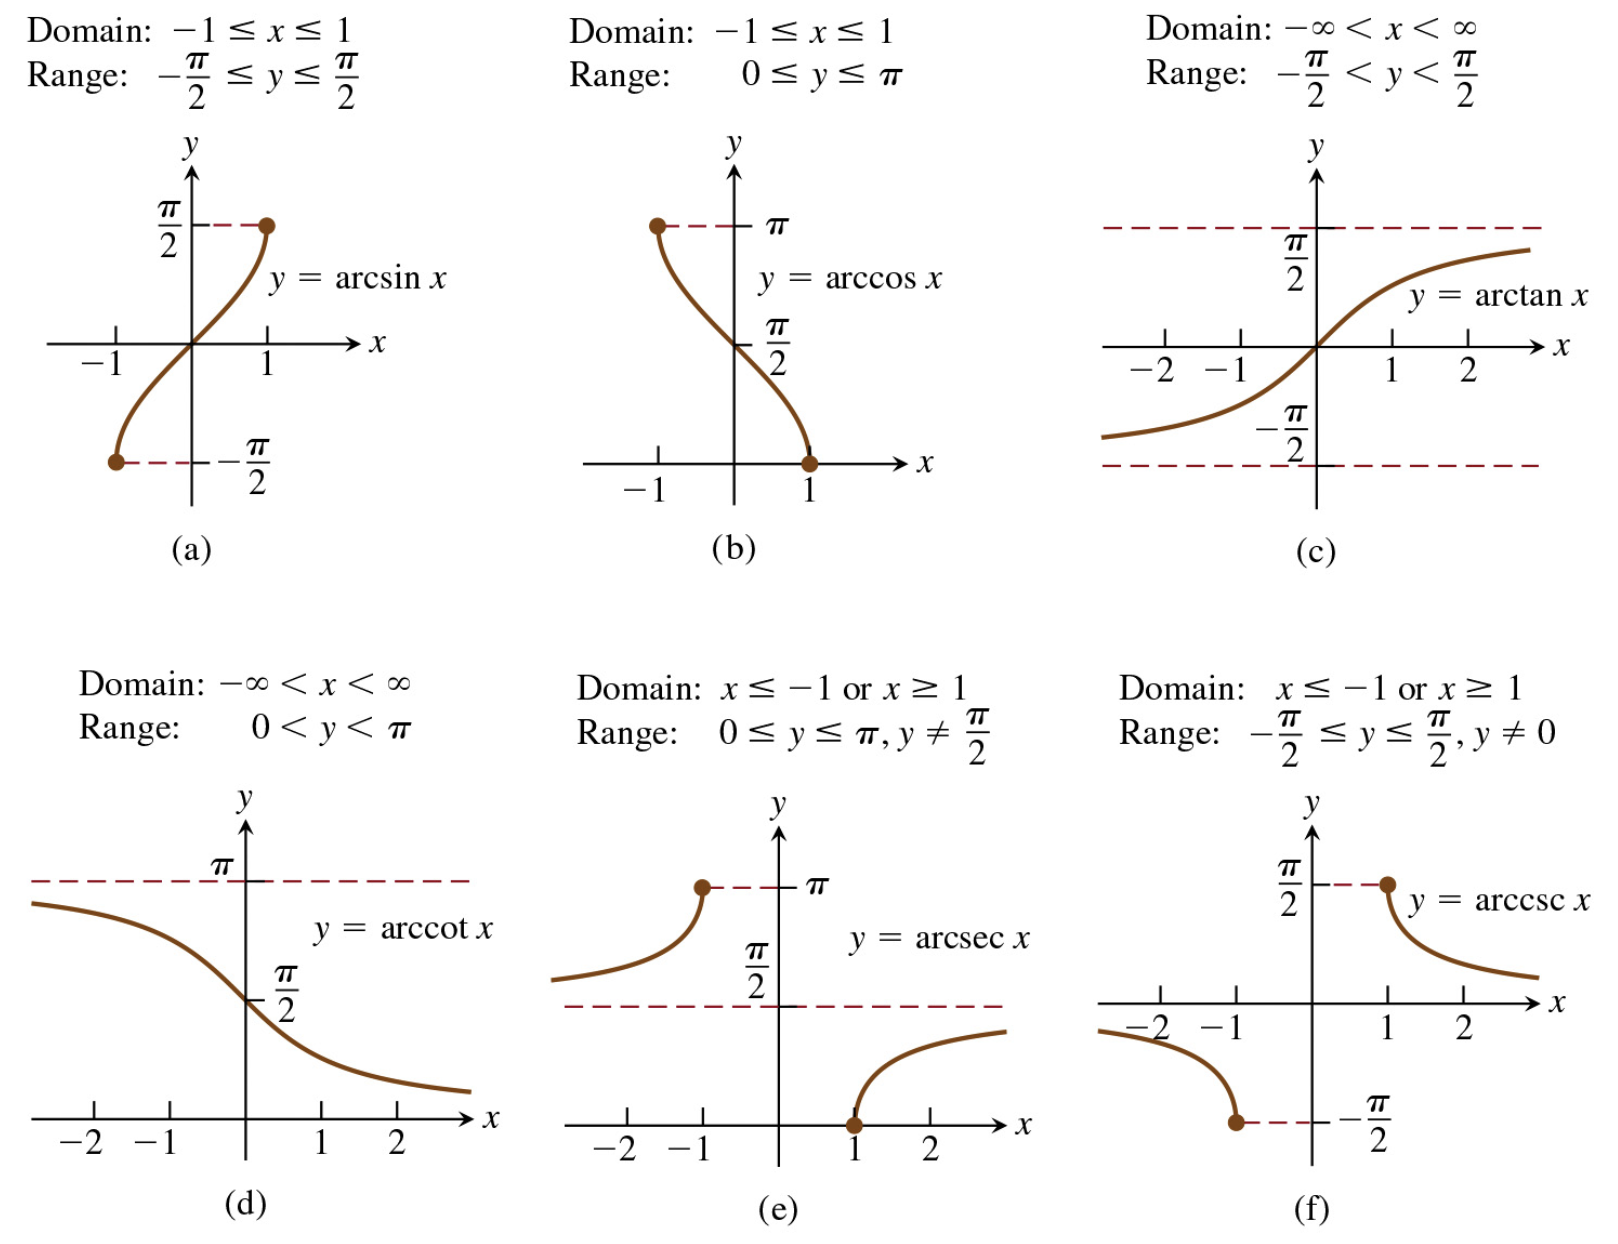
\includegraphics[width=6.5in]{img/inverse_trig_graphs}

\newpage

\begin{example}
Evaluate the following.
\begin{enumerate}
\item $\arcsin(\sqrt 3/2)$
\vfill
\item $\arcsin(-\sqrt 2/2)$
\vfill
\item $\arccos(-1/2)$
\vfill
\item $\arcsin(\sin(5\pi/8))$
\vfill
\end{enumerate}
\end{example}

\newpage

\begin{theorem}
\begin{align}
\frac{\dee}{\dee x}\arcsin x &= \frac{1}{\sqrt{1-x^2}}\quad (|x|<1),\\
\frac{\dee}{\dee x}\arccos x &= \frac{-1}{\sqrt{1-x^2}}\quad (|x|<1),\\
\frac{\dee}{\dee x}\arctan x &= \frac{1}{1+x^2},\\
\frac{\dee}{\dee x}\arccsc x &= \frac{-1}{|x|\sqrt{x^2-1}}\quad (|x|>1),\\
\frac{\dee}{\dee x}\arcsec x &= \frac{1}{|x|\sqrt{x^2-1}}\quad (|x|>1),\\
\frac{\dee}{\dee x}\arccot x &= \frac{-1}{1+x^2}.
\end{align}
\end{theorem}

\begin{proof}\,

\vspace{3.5in}
\end{proof}

\begin{corollary}
\begin{align}
\int \frac{\dee x}{\sqrt{1-x^2}} &= \arcsin x + C\quad (|x|<1),\\
\int \frac{\dee x}{1+x^2} &= \arctan x + C,\\
\int \frac{\dee x}{|x|\sqrt{x^2-1}} &= \arcsec|x| + C\quad (|x|>1).
\end{align}
\end{corollary}

\newpage

\begin{example}
Compute $\dee y/\dee x$ if $y=\arcsin x^2$.
\end{example}
\vfill

\begin{example}
Evaluate the following.
\begin{enumerate}
\item $\DS\int_{\sqrt 2/2}^{\sqrt 3/2}\frac{\dee x}{\sqrt{1-x^2}}$
\vfill
\item $\DS\int\frac{\dee x}{\sqrt{3-4x^2}}$
\vfill
\end{enumerate}
\end{example}

\newpage

\begin{example}
Compute the following integrals.
\begin{enumerate}
\item $\DS\int\frac{\dee x}{\sqrt{\E^{2x}-6}}$
\vfill
\item $\DS\int\frac{\dee x}{\sqrt{4x-x^2}}$
\vfill
\item $\DS\int\frac{\dee x}{4x^2+4x+2}$
\vfill
\end{enumerate}
\end{example}


\setcounter{equation}{0}

%!TEX root =  main.tex

\lectureheader{162}{Calculus II}{Hyperbolic functions}{\textit{Thomas' Calculus}  7.7}

\begin{definition}
We define the \textbf{hyperbolic sine} by the rule
\begin{equation*}
\sinh x = \frac{\E^x-\E^{-x}}{2} \quad (x\in\R)
\end{equation*}
and the \textbf{hyperbolic cosine} by the rule
\begin{equation*}
\cosh x = \frac{\E^x+\E^{-x}}{2} \quad (x\in\R).
\end{equation*}
\end{definition}

\begin{remark}\,
\begin{itemize}
\item These functions are affectionately referred to as ``cinch" and ``kosh."
\item The ordinary sine and cosine are sometimes called ``circular" functions because they parameterize circles.
If $t\in [0,2\pi)$, then the point $(x,y) = (\cos t, \sin t)$ lies on the circle
\begin{equation*}
x^2+y^2=1.
\end{equation*}
\item These hyperbolic analogues parameterize hyperbolas.
If $t\in (-\infty,\infty)$, then the point $(x,y)=(\cosh t, \sinh t)$ lies on the right branch of the hyperbola
\begin{equation*}
x^2-y^2=1.
\end{equation*}
\end{itemize}
\end{remark}

\begin{definition}
We define the \textbf{hyperbolic tangent} by the rule
\begin{equation*}
\tanh x = \frac{\sinh x}{\cosh x} \quad (x\in \R),
\end{equation*}
the \textbf{hyperbolic cosecant} by the rule
\begin{equation*}
\csch x = \frac{1}{\sinh x} \quad (x\ne 0),
\end{equation*}
the \textbf{hyperbolic secant} by the rule
\begin{equation*}
\sech x = \frac{1}{\cosh x} \quad (x\in\R),
\end{equation*}
and the \textbf{hyperbolic cotangent} by the rule
\begin{equation*}
\coth x = \frac{\cosh x}{\sinh x} \quad (x\ne 0).
\end{equation*}
\end{definition}

\newpage

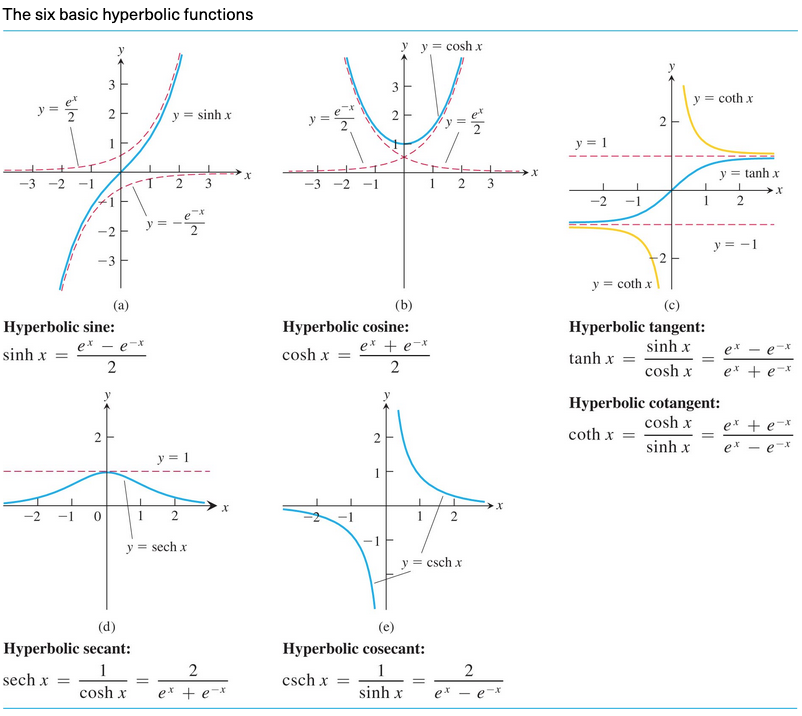
\includegraphics[width=6.5in]{img/hyperbolic_graphs}

\newpage

\begin{theorem}
For all $x$ where both sides of the identity are defined we have 
\begin{align}
\cosh^2 x -\sinh^2 x &= 1, \label{hyperbolic trig identity}\\ 
1-\tanh^2x &=\sech^2 x,\\
\coth^2 x -1&=\csch^2 x,\\
\sinh 2x &= 2\sinh x\cosh x,\\
\cosh 2x &=\cosh^2x + \sinh^2 x,\\
\cosh^2 x&=\frac{\cosh 2x + 1}{2},\\
\sinh^2 x&=\frac{\cosh 2x - 1}{2}.
\end{align}
\end{theorem}
\ifdefined\SOLUTION
\SOLUTION[Proof of \eqref{hyperbolic trig identity}] {
For all $x\in (-\infty, \infty)$,
\begin{align*}
    \cosh^2{x} - \sinh^2{x} &= \left(\frac{\E^x+\E^{-x}}{2}\right)^2 - \left(\frac{\E^x-\E^{-x}}{2}\right)^2 \\
    &= \frac{\E^{2x} + 1 + 1 + \E^{-2x}}{4} - \frac{\E^{2x} + 1 + 1 + \E^{-2x}}{4} \\
    &= \frac{(\E^{2x} + 1 + 1 + \E^{-2x}) - (\E^{2x} + 1 + 1 + \E^{-2x})}{4} \\
    &= \frac{4}{4} \\
    &= 1. \\
\end{align*}
}
\else
\begin{proof}[Proof of \eqref{hyperbolic trig identity}]\,

\vspace{5in}
\end{proof}
\fi
\newpage

\begin{theorem}
\begin{align}
\frac{\dee}{\dee x}\sinh x &= \cosh x\quad (x\in\R)\label{sinh derivative}\\
\frac{\dee}{\dee x}\cosh x &= \sinh x\quad (x\in\R)\\
\frac{\dee}{\dee x}\tanh x &= \sech^2 x\quad (x\in\R) \label{sech derivative}\\
\frac{\dee}{\dee x}\csch x &= -\csch x\coth x\quad (x\ne 0)\\
\frac{\dee}{\dee x}\sech x &= -\sech x\tanh x\quad (x\in \R)\\
\frac{\dee}{\dee x}\coth x &= -\csch^2 x\quad (x\ne 0)
\end{align}
\end{theorem}
\begin{remark}
Of course, each of these gives rise to a corresponding integral formula.
\end{remark}
\ifdefined\SOLUTION
\SOLUTION[Proof of \eqref{sech derivative}]{
For $x\in (-\infty, \infty)$,
\begin{align*}
\frac{\dee}{\dee x}\sech{x} 
	&= \frac{\dee}{\dee x} (\cosh{x})^{-1}\\
    &= -(\cosh{x})^{-2}\cdot\frac{\dee}{\dee x}\cosh{x} \\
    &= -(\cosh{x})^{-2}\sinh{x}\\ %\quad \text{(by~\eqref{sinh derivative})} \\
    &=-\tanh(x)\sech(x). 
\end{align*}
}
\else
\begin{proof}[Proof of \eqref{sech derivative}]\,

\vspace{5in}
\end{proof}
\fi

\newpage

\begin{example}
Compute $\dee y/\dee x$ if $y=\tanh \sqrt{1+x^2}$.
\end{example}
\ifdefined\SOLUTION
\SOLUTION[Solution]{
\begin{align*}
    \frac{\dee y}{\dee x} &= \left(\sech^2{\sqrt{1+x^2}}\right)\cdot\frac{\dee}{\dee x}(1+x^2)^\frac{1}{2} \\
    &= \left(\sech^2{\sqrt{1+x^2}}\right)\cdot\frac{1}{2}(1+x^2)^{-1/2}\cdot\frac{\dee}{\dee x}(1+x^2) \\
    &=  \frac{\left(\sech^2{\sqrt{1+x^2}}\right)}{2\sqrt{1+x^2}}\cdot 2x \\
    &= \frac{x\sech^2{\sqrt{1+x^2}}}{\sqrt{1+x^2}}. 
\end{align*}
}
\else
\fi
\vfill

\begin{example}
Compute $\DS\int\sinh^2 x\dee x$
\end{example}
\ifdefined\SOLUTION
\SOLUTION[Solution]{
One way to evaluate this integral is 
\begin{align*}
    \int\sinh^2 x\dee x &= \int\left(\frac{\E^x+\E^{-x}}{2}\right)^2\dee x \\
    &= \frac{1}{4}\int(\E^{2x} - 2 + \E^{-2x})\dee x \\
    &= \frac{1}{4}\left[ \frac{1}{2}\E^{2x} - 2x - \frac{1}{2}\E^{-2x} \right] + C \\
    &= \frac{1}{4}\left[ \sinh{2x} - 2x \right] + C.
\end{align*}
Another way to evaluate this integral is 
\begin{align*}
    \int\sinh^2 x\dee x &= \int\frac{\cosh{(2x} - 1)}{2}\dee x \\
    &= \frac{1}{2} \left[ \frac{1}{2}\sinh{(2x)} - x \right] + C \\
    &= \frac{1}{4}\sinh{(2x)} - \frac{1}{2}x + C.
\end{align*}
}
\else
\fi
\vfill

\newpage

\begin{example}
What is the domain/range of $y=\sinh x$?
Where can we invert it?
\end{example}
\ifdefined\SOLUTION
\SOLUTION[Solution]{
Since $\sinh(x) = \frac{\E^x-\E^{-x}}{2}$, we see that $\dom(\sinh) = (-\infty, \infty)$ and $\rng(\sinh) = (-\infty, \infty)$.  
Now note that
\begin{equation*}
    \frac{\dee}{\dee x}\sinh{x} = \cosh{x} = \frac{\E^x+\E^{-x}}{2} > 0
\end{equation*}
for all $x\in (-\infty, \infty)$.
Therefore, $\sinh{x}$ is 1-1 and thus invertible everywhere.  So, $\arcsinh{x} = \sinh^{-1}{x}$ exists and $\dom(\arcsinh) = (-\infty, \infty)$ and $\rng(\arcsinh) = (-\infty, \infty)$.
}
\else
\fi
\vfill

\begin{example}
What is the domain/range of $y=\cosh x$?
Where can we invert it?
\end{example}
\ifdefined\SOLUTION
\SOLUTION[Solution]{
Since $\cosh(x) = \frac{\E^x+\E^{-x}}{2}$, we see that $\dom(\cosh) = (-\infty,\infty)$ and $\rng(\cosh) = [1, \infty)$.
Now note that
\begin{equation*}
    \frac{\dee}{\dee x}\cosh{x} = \sinh{x} = \frac{\E^x-\E^{-x}}{2} > 0 
\end{equation*}
for all $x\in [0,\infty)$.
So, we can invert the right half of cosh, i.e., $\cosh^{-1}{x}$ exists, but $\dom(\cosh^{-1}) = [1, \infty)$ and $\rng(\cosh^{-1}) = [0, \infty).$
}
\else
\fi
\vfill

\newpage

\begin{definition}
The six ``inverse" hyperbolic functions are defined by the rules:
\begin{enumerate}
\item $y=\sinh^{-1} x\quad (x\in\R) \iff \sinh y = x\quad (y\in\R)$.
\item $y = \cosh^{-1} x\quad (x\ge 1) \iff \cosh y = x\quad (0\le y<\infty)$.
\item $y = \tanh^{-1} x\quad (|x|<1) \iff \tanh y = x\quad (y\in\R)$ 
\item $y=\csch^{-1} x\quad (x\ne 0)\iff \csch y = x\quad (y\ne 0)$.
\item $y = \sech^{-1} x\quad (0<x\le 1) \iff \sech y = x\quad (y\ge 0)$.
\item $y = \coth^{-1} x\quad (|x|>1) \iff \coth y = x\quad (y\ne 0)$.
\end{enumerate}
\end{definition}
\begin{remark}\,
\begin{itemize}
\item Four of these are ``true" inverses while the other two are only ``partial" inverses.
Can you figure out which?
\item We also use the notation $\arcsinh x = \sinh^{-1} x$, etc.
\end{itemize}
\end{remark}

\begin{theorem}
\begin{align}
\frac{\dee}{\dee x}\sinh^{-1} x & = \frac{1}{\sqrt{1+x^2}}\label{inverse sinh derivative}\\
\frac{\dee}{\dee x}\cosh^{-1} x & = \frac{1}{\sqrt{x^2-1}}\quad (x>1)\\
\frac{\dee}{\dee x}\tanh^{-1} x & = \frac{1}{1-x^2}\quad (|x|<1)\\
\frac{\dee}{\dee x}\csch^{-1} x &=\frac{-1}{|x|\sqrt{1+x^2}}\quad (x\ne 0) \label{inverse csch derivative} \\
\frac{\dee}{\dee x}\sech^{-1} x & = \frac{-1}{x\sqrt{1-x^2}}\quad (0<x<1)\\
\frac{\dee}{\dee x}\coth^{-1} x & = \frac{1}{1-x^2}\quad (|x|>1)
\end{align}
\end{theorem}
\ifdefined\SOLUTION
\SOLUTION[Proof of \eqref{inverse sinh derivative}]{
First observe that
\begin{equation*}
\sinh(\sinh^{-1}(x)) = x \quad (x\in\R).  
\end{equation*}
Differentiating both sides, we find that
\begin{equation*}
\cosh(\sinh^{-1} x)\frac{\dee}{\dee x}\sinh^{-1} x = 1.
\end{equation*}
Dividing, we have
\begin{equation*}
\frac{\dee}{\dee x}\sinh^{-1} x = \frac{1}{\cosh(\sinh^{-1} x)}.
\end{equation*}
Since $\cosh(z)>0$ for all $z\in\R$, it follows that
\begin{equation*}
\cosh(\sinh^{-1} x) = |\cosh(\sinh^{-1} x)|
 = \sqrt{\cosh^2(\sinh^{-1} x)}
 = \sqrt{1+\sinh^2(\sinh^{-1} x)}
 = \sqrt{1+x^2}.
\end{equation*}
Therefore,
\begin{equation*}
\frac{\dee}{\dee x}\sinh^{-1} x = \frac{1}{\sqrt{1+x^2}}.
\end{equation*}
}
\else
\begin{proof}[Proof of \eqref{inverse sinh derivative}]\,

\vspace{2.75in}
\end{proof}
\fi

\newpage

\begin{theorem}
\begin{align}
\int\frac{\dee x}{\sqrt{1+x^2}} &= \sinh^{-1} x + C;\\
\int\frac{\dee x}{\sqrt{x^2-1}} & = \cosh^{-1} x + C\quad (x>1);\\
\int\frac{\dee x}{1-x^2} 
&=\begin{cases}
\tanh^{-1} x + C& \text{if } |x|<1,\\
\coth^{-1} x + C& \text{if } |x|>1;
\end{cases}\\
\int\frac{\dee x}{x\sqrt{1-x^2}} &= -\sech^{-1} x + C\quad (0<x<1);\\
\int\frac{\dee x}{x\sqrt{1+x^2}} &=-\csch^{-1} |x| + C\quad (x\ne 0).
\end{align}
\end{theorem}

\begin{example}
Evaluate $\DS\int_0^1\frac{2\dee x}{\sqrt{3+4x^2}}$.
\end{example}
\ifdefined\SOLUTION
\SOLUTION[Solution]{
First note that
\begin{equation*}
    \int_0^1\frac{2\dee x}{\sqrt{3+4x^2}}
    = \int_0^1\frac{2\dee x}{\sqrt{3}\sqrt{1 + \left( \frac{2x}{\sqrt{3}} \right)^2}}.
\end{equation*}
Now let $u = \frac{2x}{\sqrt 3}$ so that $\dee u = \frac{2}{\sqrt 3}\dee x$.  
Furthermore, if $x = 0$, then $u = 0$, and if $x = 1$, then $u = \frac{2}{\sqrt{3}}$.
Making the substitution gives
\begin{equation*}
    \int_0^{\frac{2}{\sqrt{3}}} \frac{\dee u}{\sqrt{1+u^2}}
    = \arcsinh{\frac{2}{\sqrt 3}} - \arcsinh{0}
    = \arcsinh{\frac{2}{\sqrt 3}}.
\end{equation*}
}
\else
\fi

\setcounter{equation}{0}

%!TEX root =  main.tex

\lectureheader{MATH 162}{Calculus II}{Relative orders}{\textit{Thomas' Calculus} \textsection 7.8}

\begin{remark}\,
\begin{itemize}
\item It is often necessary to compare the relative size of two functions for ``large" $x$.
\item In practice, we are usually comparing a complicated/exotic function to a simpler/more familiar one.
\item This sort of thing comes up all the time when analyzing the efficiency of algorithms and the long-term behavior of other mathematical models.
\end{itemize}
\end{remark}

\begin{definition}
Let $f$ and $g$ be functions that are defined for all $x$ sufficiently large.
We say that $f$ is \textbf{at most the order of} $g$ as $x\to \infty$, and we write
\begin{equation*}
f(x) = O(g(x)) \text{ as } x\to \infty
\end{equation*}
or we write
\begin{equation*}
f(x)\ll g(x) \text{ as } x\to \infty,
\end{equation*}
if there are constants $C, M>0$ so that $|f(x)|\le C g(x)$ for all $x\ge M$.
\end{definition}
\begin{remark}\,
\begin{itemize}
\item The constant $C$ in the definition is called the \textbf{implicit constant} since it does not appear explicitly in either notation.
\item The first notation was invented by Bachmann and Landau while the second notation was invented by Vinogradov.
\item \textit{Thomas' Calculus} (your textbook) does not recognize the second notation.
\item Your professor prefers the Vinogradov notation for at least the following reasons.
\begin{enumerate}
\item If written sloppily, big-Oh is easily confused with little-Oh.  See below.
\item The $\ll$ symbol reminds us that what really underlies the notation is an inequality.
\item We are used to statements with equals signs being symmetric, but this is not necessarily so with the equals sign in the big-Oh notation.
\item Occasionally, students will confuse $O$ with a function and think we are talking about composition of functions.
\end{enumerate}
\item Caution: To say that $f(x) = O(g(x))$ as $x\to \infty$ does not necessarily imply that $g(x)$ is ever larger than $f(x)$.
\end{itemize}
\end{remark}

\newpage

\begin{example}\label{big-oh example}
Show that $x+\sin x = O(x)$ as $x\to\infty$.
\end{example}

\newpage

\begin{definition}
Let $f$ and $g$ be functions that are positive for all $x$ sufficiently large.
We say that $f$ is \textbf{of the same order as} $g$ as $x\to \infty$, and we write
\begin{equation*}
f(x) = \Theta(g(x)) \text{ as } x\to\infty
\end{equation*}
or we write
\begin{equation*}
f(x) \asymp g(x) \text{ as } x\to \infty,
\end{equation*}
if $f(x)\ll g(x)$ and $g(x)\ll f(x)$ as $x\to \infty$.
\end{definition}

\begin{remark}
\textit{Thomas' Calculus} (your textbook) does not recognize either of these notations, but the concept is still there.
\end{remark}

\begin{theorem}
If $L$ is a nonzero real number and $\DS\lim_{x\to\infty}\frac{f(x)}{g(x)} = L$, then $f(x)\asymp g(x)$ as $x\to\infty$.
\end{theorem}


\begin{example}
Show that $(\sqrt{x+4}+\cos x)^3\asymp x^{3/2}$ as $x\to\infty$.
\end{example}

\newpage

\begin{remark}\,
\begin{itemize}
\item In the previous example, we used a limit to show that $(\sqrt{x+4}+\cos x)^3\asymp x^{3/2}$ as $x\to\infty$.
\item In other words, we showed that
\begin{equation*}
x^{3/2} \ll (\sqrt{x+4}+\cos x)^3\ll x^{3/2} \text{ as } x\to\infty.
\end{equation*}
\item In other words, $f(x) = (\sqrt{x+4}+\cos x)^3$ is trapped between to multiples of $g(x)=x^{3/2}$ for all sufficiently large $x$.
\item By using the limit, we were able to bypass the need to work out
\begin{enumerate}
\item which constant multiples we wanted to use, and
\item how large $x$ needs to be so that the inequalities ``kick in."
\end{enumerate}
\item The graph below indicates a choice of constants that we could probably use if we were willing to engage in finer analysis of inequalities as in Example~\ref{big-oh example}.
\end{itemize}
\end{remark}

\begin{figure}[H]
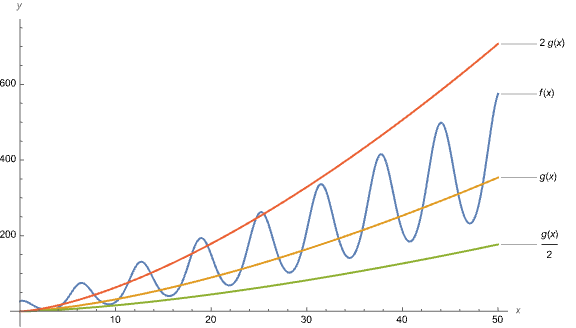
\includegraphics[width=6.5in]{img/example2}\caption{$f(x) = (\sqrt{x+4}+\cos x)^3$ and $g(x) = x^{3/2}$}
\end{figure}

\newpage

\begin{example}
Compare the growth rates of $\E^x$ and $\cosh x$ as $x\to\infty$.
\end{example}

\newpage

\begin{definition}
Let $f$ and $g$ be functions that are defined for all $x$ sufficiently large.
We say that $f$ is \textbf{of smaller order than} $g$ as $x\to \infty$, and we write
\begin{equation*}
f(x) = o(g(x)) \text{ as } x\to \infty
\end{equation*}
or we write
\begin{equation*}
f(x) \lll g(x) \text{ as } x\to\infty,
\end{equation*}
if
\begin{equation*}
\lim_{x\to\infty}\frac{f(x)}{g(x)} = 0.
\end{equation*}
\end{definition}

\begin{remark}\,
\begin{itemize}
\item If $f(x)\lll g(x)$ as $x\to\infty$, then the definition of limit implies that for every $\epsilon>0$, there is an $M>0$ so that
\begin{equation*}
x\ge M\implies |f(x)|\le \epsilon |g(x)|,
\end{equation*}
i.e., $|f(x)|$ is \underline{eventually} smaller than every positive multiple of $|g(x)|$.
%\item The first notation was invented by Bachmann and Landau, and it is read ``$f(x)$ is little-Oh of $g(x)$ as $x$ tends to infinity."
%\item The second notation was invented by Vinogradov, and it is read ``$f(x)$ is less-than-less-than-less-than $g(x)$ as $x$ tends to infinity."
\item \textit{Thomas' Calculus} (your textbook) does not recognize the second notation.
\item If $\DS\lim_{x\to\infty}\frac{f(x)}{g(x)} = \infty$, then it follows that $f(x)\ggg g(x)$ as $x\to\infty$.
\end{itemize}
\end{remark}

\begin{example}
Show that $x^2\lll \E^x$ as $x\to\infty$.
\end{example}

\newpage

\begin{theorem}
For every (fixed) $\delta>0$, 
\begin{equation*}
\ln x\lll x^\delta
\end{equation*}
as $x\to\infty$.
\end{theorem}
\begin{proof}\,

\vspace{6in}
\end{proof}

\newpage

\begin{remark}\,
\begin{itemize}
\item The previous theorem tells us that although $\ln x\to\infty$ as $x\to\infty$, ultimately it does so at a much slower rate than \underline{every} power function.
\item Although, $\ln x$ is ``winning the race" for a long time, $x^{1/4}$ will \textit{eventually} leave $\ln x$ in its dust.
\end{itemize}
\end{remark}

\begin{figure}[H]
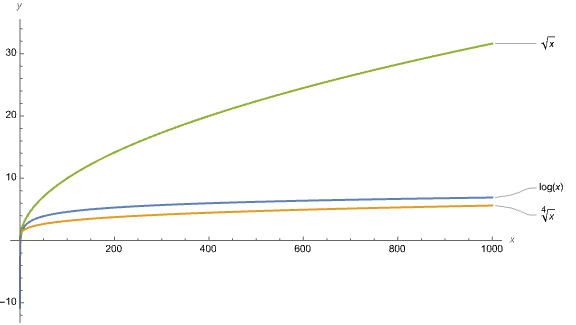
\includegraphics[width=6in]{img/log-growth}
%\begin{tikzpicture}
%\pgfplotsset{height=0.35\textheight}
%\begin{axis}[axis lines=middle, xlabel = $x$, ylabel=$y$]
%\addplot[domain=0:1000, red, line width=2pt, samples=100]{sqrt(x)};
%\addlegendentry{$y=x^{1/2}$}
%\addplot[domain=0:1000,  green, line width=2pt, samples=100]{x^(1/4)};
%\addlegendentry{$y= x^{1/4}$}
%\addplot[domain=0:1000,  blue, line width=2pt, samples=100]{ln(x)};
%\addlegendentry{$y=\ln x$}
%\end{axis}
%\end{tikzpicture}
\end{figure}

\begin{figure}[H]
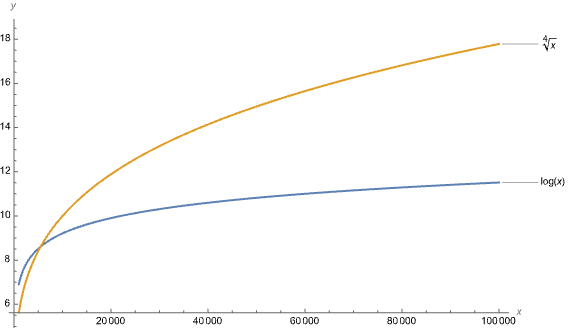
\includegraphics[width=6in]{img/log-growth2}
%\begin{tikzpicture}
%\pgfplotsset{height=0.35\textheight}
%\begin{axis}[axis lines=left, xlabel = $x$, ylabel=$y$]
%\addplot[domain=0:100000,  green, line width=2pt, samples=100]{x^(1/4)};
%\addlegendentry{$y= x^{1/4}$}
%\addplot[domain=0:100000,  blue, line width=2pt, samples=100]{ln(x)};
%\addlegendentry{$y=\ln x$}
%\end{axis}
%\end{tikzpicture}
\end{figure}


\newpage

\begin{definition}
Let $f$ and $g$ be functions that are defined for all $x$ sufficiently large.
We say that $f$ is \textbf{asymptotic to} $g$ as $x\to \infty$, and we write
\begin{equation*}
f(x) \sim g(x) \text{ as } x\to \infty
\end{equation*}
if
\begin{equation*}
\lim_{x\to\infty}\frac{f(x)}{g(x)} = 1.
\end{equation*}
\end{definition}

\begin{remark}\,
\begin{itemize}
\item The above definition says that $f$ and $g$ have an even closer relationship than merely having the same order.
\item To say that $f(x)\sim g(x)$ as $x\to \infty$  is to say that $g(x)$ is a ``good approximation" to $f(x)$ in the sense that the \underline{relative error} can be made arbitrarily small by choosing a large enough $x$, i.e., 
\begin{equation*}
\left|\frac{f(x) - g(x)}{f(x)}\right|\to 0
\end{equation*}
as $x\to\infty$.
\item \textit{Thomas' Calculus} (your textbook) does not mention this concept at all, but it is extremely useful.
\end{itemize}
\end{remark}

\begin{example}
Show that $\sinh x\sim \frac{1}{2}\E^x$ as $x\to\infty$.
\end{example}

\setcounter{equation}{0}


%!TEX root =  main.tex

\lectureheader{162}{Calculus II}{Integration by parts}{\textit{Thomas' Calculus} \textsection 8.2}

\begin{mdframed}
\begin{minipage}{0.5\linewidth}
\begin{enumerate}
%\item $\DS\int \big(f(x) + g(x)\big)\dee x = \int f(x)\dee x + \int g(x)\dee x$
\item $\DS\int x^n\dee x = \frac{x^{n+1}}{n+1}+C\quad (n\ne -1)$
\item $\DS\int\frac{\dee x}{x} = \ln|x| + C$
\item $\DS\int\E^x\dee x = \E^x + C$
\item $\DS\int\sinh x\dee x = \cosh x+C$
\item $\DS\int\cosh x\dee x=\sinh x + C$
\item $\DS\int\frac{\dee x}{\sqrt{1-x^2}} = \arcsin x + C$
\item $\DS\int\frac{\dee x}{1+x^2} = \arctan x + C$
\item $\DS\int\frac{\dee x}{x\sqrt{x^2-1}} = \arcsec|x|+C$
\item $\DS\int\frac{\dee x}{\sqrt{1+x^2}} = \sinh^{-1} x + C$
\item $\DS\int\frac{\dee x}{\sqrt{x^2-1}} = \cosh^{-1} x + C$
\end{enumerate}
\end{minipage}
\begin{minipage}{0.5\linewidth}
\begin{enumerate}
\setcounter{enumi}{10}
\item $\DS\int\sin x\dee x=-\cos x + C$
\item $\DS\int\cos x\dee x=\sin x +C$
\item $\DS\int\tan x\dee x=\ln|\sec x| + C$
\item $\DS\int\csc x\dee x=-\ln|\csc x+\cot x| + C$
\item $\DS\int\sec x\dee x=\ln|\sec x+\tan x|+C$
\item $\DS\int\cot x\dee x=\ln|\sin x| +C$
\item $\DS\int\sec^2 x\dee x = \tan x + C$
\item $\DS\int\csc x\cot x\dee x=-\csc x+C$
\item $\DS\int\sec x\tan x\dee x = \sec x+C$
\item $\DS\int\csc^2 x\dee x = -\cot x+C$
\end{enumerate}
\end{minipage}
\end{mdframed}

%\begin{example}
%Evaluate $\DS\int_3^5\frac{2x-3}{\sqrt{x^2-3x+1}}\dee x$.
%\end{example}
%
%\newpage
%
%\begin{example}
%Compute the following.
%\begin{enumerate}
%\item $\DS\int\frac{\dee x}{\sqrt{8x-x^2}}$
%\vfill
%\item $\DS\int\big(\cos x\sin 2x + \sin x\cos 2x\big)\dee x$
%\vfill
%\end{enumerate}
%\end{example}
%
%\newpage
%
%\begin{example}
%Evaluate the following.
%\begin{enumerate}
%\item $\DS\int_0^{\pi/4}\frac{\dee x}{1-\sin x}$
%\vfill
%\item $\DS\int\frac{3x^2-7x}{3x+2}\dee x$
%\vfill
%\end{enumerate}
%\end{example}
%
%\newpage
%
%\begin{example}
%Determine the following.
%\begin{enumerate}
%\item $\DS\int\frac{3x+2}{\sqrt{1-x^2}}\dee x$
%\vfill
%\item $\DS\int\frac{\dee x}{(1+\sqrt x)^3}$
%\vfill
%\end{enumerate}
%\end{example}
%
%\newpage

\begin{remark}\,
\begin{itemize}
\item Viewing the chain rule (for differentiation) as a fact about integration led to the technique of $u$-substitution.
\item Similarly, viewing the product rule as a fact about integration leads to a technique known as \textbf{integration by parts}.
\item In particular, the formula
\begin{equation*}
\frac{\dee }{\dee x}f(x)g(x) = g(x)\frac{\dee}{\dee x}f(x) + f(x)\frac{\dee}{\dee x}g(x)
\end{equation*}
is rearranged as
\begin{equation*}
f(x)\frac{\dee}{\dee x}g(x) = \frac{\dee }{\dee x}f(x)g(x) - g(x)\frac{\dee}{\dee x}f(x) 
\end{equation*}
and then integrated to reveal
\begin{equation*}
\int f(x)\frac{\dee}{\dee x}g(x)\dee x = f(x)g(x) - \int g(x)\frac{\dee}{\dee x}f(x) \dee x.
\end{equation*}
\item Putting $u=f(x)$ and $v=g(x)$, we usually remember this in the convenient form
\begin{equation}
\int u\dee v = uv - \int v\dee u.
\end{equation}
\end{itemize}
\end{remark}

\newpage

\begin{example}
Evaluate the following.
\begin{enumerate}
\item $\DS\int x\cos x\dee x$
\vfill
\item $\DS\int\ln x\dee x$
\vfill
\end{enumerate}
\end{example}

\newpage

\begin{example}
Evaluate the following.
\begin{enumerate}
\item $\DS\int x^2\E^x\dee x$
\vfill
\item $\DS\int\E^x\cos x\dee x$
\vfill
\end{enumerate}
\end{example}

\newpage

\begin{example}
Find the area under the curve $y=x\E^x$ over the interval $[0,4]$.
\end{example}

\setcounter{equation}{0}

%!TEX root =  main.tex
\setcounter{chapter}{8}
\setcounter{section}{3}
\setcounter{theorem}{0}
\setcounter{equation}{0}

\lectureheader{162}{Calculus II}{Trigonometric integration}{\textit{Thomas' Calculus}  \thesection}

\begin{remark}
To evaluate $\int \sin^m x\cos^n x\dee x$ we have the following basic strategy.
\begin{enumerate}
\item If $m=2k+1$ is odd, then we save a factor of $\sin x\dee x = -\dee(\cos x)$ and use identity $\sin^2 x + \cos^2 x = 1$ to write
\begin{equation*}
\begin{split}
\int \sin^m x \cos^n x\dee x &= \int (\sin^2 x)^k\sin x\cos^n x\dee x \\
&= \int (1-\cos^2 x)^k\cos^n x\sin x\dee x\\
& = -\int (1-u^2)^ku^n\dee u,
\end{split}
\end{equation*}
where $u=\cos x$.
\item If $n=2k+1$ is odd, then we save a factor $\cos x\dee x = \dee(\sin x)$ and write
\begin{equation*}
\begin{split}
\int \sin^m x \cos^n x\dee x &= \int\sin^m x(\cos^2 x)^k\cos x\dee x \\
&= \int\sin^m x(1-\sin^2 x)^k\cos x\dee x \\
&= \int u^m(1-u^2)^k\dee u,
\end{split}
\end{equation*}
where $u=\sin x$.
\item If $m$ and $n$ are both even, then we reduce to lower powers using the identities
\begin{align*}
\cos^2 x = \frac{1+\cos 2x}{2},\\
\sin^2 x = \frac{1-\cos 2x}{2}.
\end{align*}
\end{enumerate}
\end{remark}

\begin{example}
Calculate $\DS\int\cos^5 x\dee x$.
\end{example}
\ifdefined\SOLUTION
\SOLUTION[Solution]{
Since we have an odd power of cosine, we save one and trade the rest for sines:
\begin{equation*}
    \int\cos^5 x\dee x
    = \int\cos^4x \cos x \dee x
    = \int (1-\sin^2 x)^2 \cos x \dee x.
\end{equation*}
Now let $u = \sin x$.  So, $\dee u = \cos x$.  
Making the substitution gives 
\begin{equation*}
\begin{split}
    \int\cos^5 x\dee x
    &=\int (1-u^2)^2\dee u\\
    &= \int 1 - 2u^2 - u^4 \dee u\\
    &= u - \frac{2}{3}u^3 - \frac{1}{5}u^5 + C\\
    &= \sin x - \frac{2}{3}(\sin x)^3 - \frac{1}{5}(\sin x)^5 + C.
\end{split}
\end{equation*}
}
\fi
\vfill

\newpage

\begin{example}
Compute $\DS\int\sin^3 x\cos^2 x\dee x$.
\end{example}
\ifdefined\SOLUTION
\SOLUTION[Solution]{
Since the power on the sine is odd, we prep for the $u$-sub by saving a sine and trading the rest for cosines:
\begin{equation*}
    \int\sin^3 x\cos^2 x\dee x
    = \int\sin^2 x\cos^2 x \sin x \dee x
    = \int(1-\cos^2 x)\cos^2 x\sin x \dee x.
\end{equation*}
Now let $u = \cos x$.  So, $\dee u = -\sin x \dee x$.  
Making the substitution gives
\begin{equation*}
\begin{split}
\int\sin^3 x\cos^2 x\dee x
   &=-\int (1-u^2)u^2\dee u
    = -\int (u^2 - u^4) \dee u\\
    &= \int (u^4 - u^2) \dee u
    = \frac{1}{5}u^5 - \frac{1}{3}u^3 + C\\
    &= \frac{1}{5}(\cos x)^5 - \frac{1}{3}(\cos x)^3 + C.
\end{split}
\end{equation*}
}
\fi
\vfill

\begin{example}
Determine $\DS\int\sin^2 x\cos^4 x\dee x$.
\end{example}
\ifdefined\SOLUTION
\SOLUTION[Solution]{
Since both powers are even, we ``power-reduce" first:
\begin{align*}
    \int\sin^2 x\cos^4 x\dee x
    &= \int \left( \frac{1-\cos{(2x)}}{2}\right)
    \left(\frac{1+\cos{(2x)}}{2}
    \right)^2 \dee x \\
    &= \frac{1}{8}\int (1- \cos^2(2x))(1+\cos(2x))\dee x \\
    &= \frac{1}{8}\int 1 + \cos(2x) - \cos^2(2x) -\cos^3(2x) \dee x \\
    &= \frac{1}{8}\left(x + \frac{1}{2}\sin(2x) - \int\cos^2(2x)\dee x - \int \cos^3(2x) \dee x
    \right) \\
    &= \frac{1}{8}\left(x + \frac{1}{2}\sin(2x) - \int\frac{1+\cos(4x)}{2}\dee x - \int (1-\sin^2(2x))\cos(2x) \dee x\right). 
\end{align*}
Now let $u = \sin(2x)$.  So, $\dee u = 2\cos(2x)\dee x$.  
Making the substitution gives 
\begin{align*}
    \int\sin^2 x\cos^4 x\dee x
    &= \frac{1}{8}\left[ x + \frac{1}{2}\sin(2x) - \frac{1}{2}\left(x + \frac{1}{4}\sin(4x)\right)  - \frac{1}{2}\int (1-u^2) \dee u
    \right] \\
    &= \frac{1}{8}\left[ x + \frac{1}{2}\sin(2x) - \frac{1}{2}\left(x + \frac{1}{4}\sin(4x)\right)  - \frac{1}{2}(u -\frac{1}{3}u^3)
    \right]  + C\\
    &= \frac{1}{8}\left[ x + \frac{1}{2}\sin(2x) - \frac{1}{2}\left(x + \frac{1}{4}\sin(4x)\right)  - \frac{1}{2}\left(\sin(2x) -\frac{1}{3}(\sin(2x))^3\right) 
    \right]+ C \\  
    &= \frac{1}{8}\left[ x + \frac{1}{2}\sin(2x) - \frac{1}{2}x + \frac{1}{8}\sin(4x)  - \frac{1}{2}\sin(2x) +\frac{1}{6}\sin(2x)^3
    \right]+ C \\ 
    &= \frac{1}{8}\left[ x - \frac{1}{2}x + \frac{1}{8}\sin(4x) +\frac{1}{6}(\sin(2x))^3 
    \right]+ C \\ 
    &= \frac{1}{16}x - \frac{1}{64}\sin(4x) + \frac{1}{48}\sin^3(2x) + C.
\end{align*}
}
\else
\fi
\vfill
\vfill

\newpage

\begin{remark}
To evaluate $\int\tan^m x\sec^n x\dee x$ we have the following basic strategy.
\begin{enumerate}
\item If $n=2k$ is even, we save a factor of $\sec^2 x\dee x = \dee(\tan x)$ and use $1+\tan^2 x = \sec^2 x$ to write
\begin{equation*}
\begin{split}
\int\tan^m x\sec^n x\dee x &= \int\tan^m x(\sec^2 x)^{k-1}\sec^2 x\dee x\\
&= \int\tan^m x(1+\tan^2 x)^{k-1}\sec^2 x\dee x\\
&= \int u^m (1+u^2)^{k-1}\dee u,
\end{split}
\end{equation*}
where $u=\tan x$.
\item If $m=2k+1$ is odd, we save a factor of $\sec x\tan x\dee x = \dee(\sec x)$ and write
\begin{equation*}
\begin{split}
\int\tan^m x\sec^n x\dee x &= \int (\tan^{2} x)^k\sec^{n-1} x\sec x\tan x\dee x\\
&= \int (\sec^{2} x -1)^k\sec^{n-1} x\sec x\tan x\dee x\\
&= \int (u^2 -1)^ku^{n-1} \dee u,
\end{split}
\end{equation*}
where $u=\sec x$.
\item The situation is not so clear-cut in the remaining cases.
Integration by parts and a little ingenuity may be required.
\end{enumerate}
\end{remark}

\begin{example}
Evaluate $\DS\int\sec^4 x\tan^4 x\dee x$.
\end{example}
\ifdefined\SOLUTION
\SOLUTION[Solution]{
\begin{equation*}
    \int\sec^4 x\tan^4 x\dee x
    = \int\sec^2 x\tan^4 x\sec^2 x\dee x 
    = \int (1+\tan^2 x)\tan^4 x\sec^2 x\dee x. 
\end{equation*}
Let $u = \tan x.$  So, $\dee u = \sec^2x\dee x$.  
Making the substitution gives 
\begin{equation*}
\begin{split}
    \int\sec^4 x\tan^4 x\dee x
    &=\int(1+u^2)u^4\dee u \\
    &= \int u^4 + u^6 \dee u\\
    &= \frac{1}{5}u^5 + \frac{1}{7}u^7 + C\\
    &= \frac{1}{5}\tan^5x + \frac{1}{7}\tan^7x + C.
\end{split}
\end{equation*}
}
\else
\fi
\vfill

\newpage

\begin{example}
Compute $\DS\int\tan^3 x\dee x$.
\end{example}
\ifdefined\SOLUTION
\SOLUTION[Solution]{
Here we have a choice of strategies.
If we notice that the power on the tangent is odd, we would prep like this:
\begin{align*}
    \int\tan^3(x)\dee x
    &= \int\frac{\tan^2x\sec x\tan x}{\sec x}\dee x \\
    &= \int \frac{(\sec^2x-1)\sec x \tan x}{\sec x}\dee x.
\end{align*}
Then we let $u = \sec x$, and so $\dee u = \sec x\tan x \dee x$.  
Making the substitution gives 
\begin{align*}
    \int\tan^3(x)\dee x
    &=\int \frac{u^2-1}{u}\dee u\\
    &= \int u - \frac{1}{u}\dee u \\
    &= \frac{1}{2}u^2 - \ln|u| + C \\
    &= \frac{1}{2}\sec^2(x) - \ln|\sec x| + C.
\end{align*}
Alternatively, we might notice that the power of secant is even.
This suggests
\begin{align*}
\int\tan^3(x)\dee x 
&= \int\frac{\tan^3 x}{\sec^2 x}\dee x
=\int\frac{\tan^3 x}{1+\tan^2 x}\dee(\tan x)
=\int\left(\tan x - \frac{\tan x}{1+\tan^2 x}\right)\dee(\tan x)\\
&=\frac{1}{2}\tan^2 x -\frac{1}{2}\int\frac{\dee(1+\tan^2 x)}{1+\tan^2 x}
=\frac{1}{2}\tan^2 x -\frac{1}{2}\ln|1+\tan^2 x| + C.
\end{align*}
A third option is 
\begin{align*}
    &= \int (\sec^2(x)-1)\tan x \dee x \\
    &= \int \sec^2(x)\tan(x)\dee x - \int\tan(x) \dee x \\
    &= \frac{1}{2}\tan^2(x) - \ln|\sec x| + C.
\end{align*}
}
\else
\fi
\vfill

\newpage

\begin{example}
Evaluate $\DS\int\tan^4 x\dee x$.
\end{example}
\ifdefined\SOLUTION
\SOLUTION[Solution]{
Note that if $u = \tan x, \dee u = \sec^2x\dee x$. 
Therefore,
\begin{align*}
    \int \tan^4x\dee x
    &= \int \tan^2x(\sec^2x-1)\dee x \\
    &= \int \tan^2x\sec^2x\dee x - \int \tan^2x\dee x \\
    &= \frac{1}{3}\tan^3x - \int (\sec^2x - 1)\dee x \\
    &= \frac{1}{3}\tan^3x - \tan x + x + C.
\end{align*}
Note that all 3 apparently different results are equivalent.
}
\else
\fi
\vfill

\begin{example}
Use integration by parts and the ``wrap-around trick" to compute $\DS\int\sec^3 x\dee x$.
\end{example}
\ifdefined\SOLUTION
\SOLUTION[Solution]{
Let $u = \sec x$ and $\dee v = \sec^2 x \dee x.$  So, $\dee u = \sec x\tan x\dee x$ and $v = \tan x$ 
Integration by parts yields 
\begin{align*}
    \int\sec^3x\dee x
    &= \sec x \tan x - \int\tan^2 x\sec x \dee x \\
    &= \sec x \tan x - \int(\sec^2x - 1)\sec x \dee x \\
    &= \sec x \tan x - \int\sec^3x\dee x + \int\sec x \dee x \\
    &= \sec x \tan x - \int\sec^3x\dee x + \ln{\left| \sec x + \tan x\right|}. 
\end{align*}
Note that we now have $-1$ times $\int\sec^3 x\dee x$ on the right, and that means that we win.
Solving for the integral we have 
\begin{equation*}
    2\int\sec^3x\dee x = \sec x\tan x + \ln{\left| \sec x + \tan x\right|} + C,
\end{equation*}
and hence
\begin{equation*}
    \int\sec^3x\dee x = \frac{1}{2}\left(\sec x\tan x + \ln{\left| \sec x + \tan x\right|}\right) + C.
\end{equation*}
}
\else
\fi
\vfill

\newpage

\begin{remark}
The identities 
\begin{align*}
\cos^2 x = \frac{1+\cos 2x}{2},\\
\sin^2 x = \frac{1-\cos 2x}{2}
\end{align*}
can also be used to eliminate pesky square roots.
\end{remark}

\begin{example}
Evaluate $\DS\int_{\pi/4}^{\pi/2}\sqrt{1+\cos 4\theta}\dee\theta$.
\end{example}
\ifdefined\SOLUTION
\SOLUTION[Solution]{
\begin{align*}
    \int_{\pi/4}^{\pi/2}\sqrt{1+\cos 4\theta}\dee\theta
    &= \int_{\pi/4}^{\pi/2}\sqrt{2\cos^2(2\theta)}\dee\theta \\
    &= \sqrt{2}\int_{\pi/4}^{\pi/2}\left| \cos(2\theta)\right| \dee \theta \\
    &= -\sqrt{2}\int_{\pi/4}^{\pi/2} \cos(2\theta)\dee \theta \\
    &= -\sqrt{2}\left[ \frac{\sin(2\theta)}{2}
    \right]_{\pi/4}^{\pi/2} \\
    &= \frac{-\sqrt{2}}{2}\left(\sin(\pi) - \sin(\pi/2)
    \right) \\
    &= -\frac{\sqrt{2}}{2}(0-1) \\
    &= \frac{\sqrt{2}}{2}
\end{align*}
}
\fi
\newpage

\begin{remark}
When integrating products of sines and cosines of differing frequencies, the identities
\begin{align*}
\sin mx\sin nx &= \frac{1}{2}\big(\cos(m-n)x - \cos(m+n)x\big),\\
\sin mx\cos nx &= \frac{1}{2}\big(\sin(m-n)x + \sin(m+n)x\big),\\
\cos mx\cos nx &= \frac{1}{2}\big(\cos(m-n)x + \cos(m+n)x\big)
\end{align*}
may be of use.
\end{remark}

\begin{example}
Evaluate $\DS\int \sin 3x\cos 5x\dee x$.
\end{example}
\ifdefined\SOLUTION
\SOLUTION{
Using the second identity above, we find that
\begin{equation*}
\begin{split}
\int \sin 3x\cos 5x\dee x 
&=\frac{1}{2}\int\left(\sin(-2x)+\sin(8x)\right)\dee x\\
&=\frac{1}{2}\left(\frac{-\cos(-2x)}{-2}+\frac{-\cos(8x)}{8}\right) + C\\
&=\frac{1}{4}\cos(2x)-\frac{1}{16}\cos(8x) + C.
\end{split}
\end{equation*}
Note that we used the fact that cosine is an even function in the last line.
}
\fi

\setcounter{equation}{0}

%!TEX root =  main.tex
\setcounter{chapter}{8}
\setcounter{section}{4}
\setcounter{theorem}{0}
\setcounter{equation}{0}

\lectureheader{162}{Calculus II}{Trigonometric substitution}{\textit{Thomas' Calculus}  \thesection}

\begin{remark}
Integrals often arise with integrands containing expressions of the form $\sqrt{a^2-x^2}$.
It is convenient to make the substitution $x=a\sin\theta$, really $\theta = \arcsin(x/a)$.  
Why?
\end{remark}

\ifdefined\SOLUTION
\SOLUTION{
Assume $a>0$, and let $x=a\sin\theta$, i.e., let $\theta = \arcsin(x/a)\in [-\pi/2, \pi/2]$.
Then the usual Pythagorean identity gives that
\begin{equation*}
\sqrt{a^2-x^2} = \sqrt{a^2 - a^2\sin^2\theta}
=a\sqrt{1-\sin^2\theta} 
=a\sqrt{\cos^2\theta}
=a|\cos\theta|.
\end{equation*}
However, since $\theta\in [-\pi/2, -\pi/2]$, it follows that $\cos\theta\ge 0$.
Therefore,
\begin{equation*}
\sqrt{a^2-x^2} = a\cos\theta,
\end{equation*}
and so we can trade integrating squareroots for trigonometric integration, which we just practiced.
However, once the integration is all over, we have to convert our result to an expression in terms of $x$, not $\theta$.
Usually the easiest way to do that is to draw/imagine the reference triangle for the relation $x=a\sin\theta$ which has opposite side $x$, hypotenuse $a$, and adjacent side $\sqrt{a^2-x^2}$.
}
\fi

\newpage

\begin{example}
Evaluate $\DS\int\frac{x^2\dee x}{\sqrt{9-x^2}}$.
\end{example}

\ifdefined\SOLUTION
\SOLUTION{
Let $x=3\sin\theta$ so that $\dee x = 3\cos\theta \dee\theta$ and
\begin{equation*}
\sqrt{9-x^2} = \sqrt{9-9\sin^2\theta} = 3\cos\theta.
\end{equation*}
Whence
\begin{equation*}
\int\frac{x^2\dee x}{\sqrt{9-x^2}} = \int\frac{9\sin^2\theta}{3\cos\theta}3\cos\theta\dee\theta
=9\int\sin^2\theta\dee\theta
=\frac{9}{2}\int(1-\cos 2\theta)\dee\theta
=\frac{9}{2}\left(\theta -\frac{1}{2}\sin 2\theta\right)+C.
\end{equation*}
Now we need to express our result in terms of $x$.
We already know that $\sin\theta = x/3$, 
and from that we deduce that $\theta = \arcsin(x/3)$ and $\cos\theta =\frac{1}{3}\sqrt{9-x^2}$.
Thus, we can use the trigonometric identity $\sin 2\theta = 2\sin\theta\cos\theta$ to see that
\begin{equation*}
\sin 2\theta = \frac{2}{9}x\sqrt{9-x^2}.
\end{equation*}
Therefore, 
\begin{equation*}
\int\frac{x^2\dee x}{\sqrt{9-x^2}} 
=\frac{9}{2}\left(\theta -\frac{1}{2}\sin 2\theta\right)+C
=\frac{9}{2}\left(\arcsin(x/3) - \frac{x\sqrt{9-x^2}}{9}\right) +C.
\end{equation*}
}
\fi

\newpage

\begin{remark}
For integrands containing expressions of the form $\sqrt{a^2+x^2}$, it is convenient to make the substitution $x=a\tan\theta$, really $\theta=\arctan(x/a)$.
Why?
\end{remark}

\ifdefined\SOLUTION
\SOLUTION{
Assume $a>0$, and let $x=a\tan\theta$, i.e., let $\theta = \arctan(x/a)\in (-\pi/2, \pi/2)$
Then the usual Pythagorean identity gives that
\begin{equation*}
\sqrt{a^2+x^2} = \sqrt{a^2 + a^2\tan^2\theta}
=a\sqrt{1+\tan^2\theta} 
=a\sqrt{\sec^2\theta}
=a|\sec\theta|.
\end{equation*}
However, since $\theta\in (\pi/2, -\pi/2)$ it follows that $\sec\theta>0$.
Therefore,
\begin{equation*}
\sqrt{a^2+x^2} = a\sec\theta.
\end{equation*}
Again, once the integration is all over, we have to convert our result to an expression in terms of $x$, not $\theta$.
Usually the easiest way to do that is to draw/imagine the reference triangle for the relation $x=a\tan\theta$ which has opposite side $x$, adjacent side $a$, and hypotenuse $\sqrt{a^2+x^2}$.
}
\fi

\newpage

\begin{example}
Compute $\DS\int\frac{\dee x}{\sqrt{4+x^2}}$.
\end{example}

\ifdefined\SOLUTION
\SOLUTION{
Let $x=2\tan\theta$ so that $\dee x = 2\sec^2\theta\dee\theta$ and
\begin{equation*}
\sqrt{4+x^2} = \sqrt{4+4\tan^2\theta} = 2\sec\theta.
\end{equation*}
Whence, 
\begin{equation*}
\int\frac{\dee x}{\sqrt{4+x^2}}
=\int\frac{2\sec^2\theta\dee\theta}{2\sec\theta}
=\int\sec\theta\dee\theta
=\ln|\sec\theta + \tan\theta| + C
=\ln\left|\frac{\sqrt{4+x^2}}{2} + \frac{x}{2}\right| + C.
\end{equation*}
}
\fi

\newpage

\begin{example}
What can a tangent substitution teach you about $\arcsinh x$?
Hint: What is the derivative?
\end{example}

\ifdefined\SOLUTION
\SOLUTION{
Recall that
\begin{equation*}
\frac{\dee}{\dee x}\arcsinh x = \frac{1}{\sqrt{1+x^2}}\quad (-\infty<x<\infty).
\end{equation*}
Now let $x=\tan\theta$ so that $\dee x = \sec^2\theta\dee\theta$ and $\sqrt{1+x^2} = \sqrt{1+\tan^2\theta} = \sec\theta$.
Whence, 
\begin{equation*}
\begin{split}
\arcsinh x 
&= \int\frac{\dee x}{\sqrt{1+x^2}}\\
&=\int\frac{\sec^2\theta\dee\theta}{\sec\theta}\\
&=\int\sec\theta\dee\theta\\
&=\ln|\sec\theta + \tan\theta| + C\\
&=\ln\left|\sqrt{1+x^2} + x\right| + C
\end{split}
\end{equation*}
for some particular constant $C$.
To determine $C$, we substitute $x=0$ which reveals that
\begin{equation*}
0=\arcsinh(0) = \ln|\sqrt{1+0^2} + 0| + C = C.
\end{equation*}
Therefore,
\begin{equation*}
\arcsinh x 
=\ln\left|\sqrt{1+x^2} + x\right|.
\end{equation*}
}
\fi

\newpage

\begin{remark}
For integrands containing expressions of the form $\sqrt{x^2-a^2}$, it is convenient\footnote{Some people prefer $x=\pm a\cosh\theta$.} to make the substitution $x=a\sec\theta$, really $\theta=\arcsec(x/a)$.
Why?
\end{remark}

\ifdefined\SOLUTION
\SOLUTION{
Assume $a>0$, and let $x=a\sec\theta$, i.e., let $\theta = \arcsec(x/a)\in [0, \pi/2)\cup (\pi/2, \pi]$
Then the usual Pythagorean identity gives that
\begin{equation*}
\sqrt{x^2-a^2} = \sqrt{a^2\sec^2\theta - a^2}
=a\sqrt{\sec^2\theta-1}
=a|\tan\theta|.
\end{equation*}
This time we aren't so fortunate when we try to remove the absolute value.
Rather we have that
\begin{equation*}
\sqrt{x^2-a^2} =
\begin{cases}
a\tan\theta & \text{if }\theta\in [0,\pi/2), \text{ i.e., } x\ge a\\
-a\tan\theta & \text{if }\theta\in (\pi/2, \pi], \text{ i.e. }, x\le a.
\end{cases}
\end{equation*}
Again, once the integration is all over, we have to convert our result to an expression in terms of $x$, not $\theta$.
Usually the easiest way to do that is to draw/imagine the reference triangle for the relation $x=a\sec\theta$ which has hypotenuse $|x|$, adjacent side $a$, and opposite side $\sqrt{x^2-a^2}$.
}
\fi

\newpage

\begin{example}
Calculate $\DS\int\frac{\dee x}{\sqrt{25x^2-4}}$.
\end{example}

\ifdefined\SOLUTION
\SOLUTION{
This time we take $5x = 2\sec\theta$ so that $5\dee x = 2\sec\theta\tan\theta\dee\theta$ and
\begin{equation*}
\sqrt{25x^2-4} = \sqrt{4\sec^2\theta - 4} = 2\sqrt{\sec^2\theta-1} = 2\sqrt{\tan^2\theta} = 2|\tan\theta|.
\end{equation*}
Whence,
\begin{equation*}
\begin{split}
\int\frac{\dee x}{\sqrt{25x^2-4}} 
&= \int\frac{\frac{2}{5}\sec\theta\tan\theta\dee\theta}{2|\tan\theta|}\\
&=\begin{cases}
\frac{1}{5}\int\sec\theta\dee\theta & \text{if } \theta\in (0,\pi/2),\\
-\frac{1}{5}\int\sec\theta\dee\theta & \text{if }\theta\in (\pi/2, \pi)
\end{cases}\\
&=\begin{cases}
\frac{1}{5}\ln|\sec\theta + \tan\theta| + C & \text{if } \theta\in (0,\pi/2),\\
-\frac{1}{5}\ln|\sec\theta + \tan\theta| + C & \text{if }\theta\in (\pi/2, \pi).
\end{cases}\\
&=\begin{cases}
\frac{1}{5}\ln\left|\frac{5x}{2} + \frac{\sqrt{25x^2-4}}{2}\right| + C & \text{if } x>2/5,\\
-\frac{1}{5}\ln\left|\frac{5x}{2} - \frac{\sqrt{25x^2-4}}{2}\right| + C & \text{if } x<-2/5.\\
\end{cases}
\end{split}
\end{equation*}
Perhaps a bit surprisingly, it turns out that expressions in the two different cases are algebraically equivalent so that
\begin{equation*}
\int\frac{\dee x}{\sqrt{25x^2-4}} 
=\frac{1}{5}\ln\left|\frac{5x}{2} + \frac{\sqrt{25x^2-4}}{2}\right| + C\quad (|x|>2/5).
\end{equation*}
}
\fi

\setcounter{equation}{0}

%!TEX root =  main.tex

\lectureheader{162}{Calculus II}{Partial fraction decomposition}{\textit{Thomas' Calculus} \textsection 8.5}

\begin{example}
Use the fact that
\begin{equation*}
\frac{5x-3}{x^2-2x-3} = \frac{3}{x-3} + \frac{2}{x+1}
\end{equation*}
to compute $\DS \int\frac{5x-3}{x^2-2x-3} \dee x$.
\end{example}


\vfill
\begin{remark}
The process of ``un-common-denominatorizing" a rational function is known as \textit{partial fraction decomposition}.
We will apply the following strategy to integrate a rational function $f(x)/g(x)$.
\begin{enumerate}
\item Use polynomial long division to write 
\begin{equation*}
\frac{f(x)}{g(x)} = q(x) + \frac{r(x)}{g(x)},
\end{equation*}
where $\deg(r)<\deg(g)$.
\item Factor the denominator $g(x)$ into linear factors (of the form $ax+b$) and irreducible quadratic factors (of the form $ax^2+bx+c$ with $b^2-4ac<0$).
\item Write the remaining proper rational function $r(x)/g(x)$ as a sum of terms of the form
\begin{equation*}
\frac{A}{(ax+b)^i}\quad\text{or}\quad\frac{Ax+B}{(ax^2+bx+c)^i}.
\end{equation*}
\end{enumerate}
\end{remark}

\newpage

\begin{remark}
If the denominator $g(x)$ factors into a product of distinct linear factors
\begin{equation*}
\begin{split}
g(x) &= \prod_{j=1}^k(a_jx+b_j)\\
& = (a_1x+b_1)(a_2x+b_2)\cdots (a_kx+b_k),
\end{split}
\end{equation*}
then we solve for constants $A_1, A_2,\dots, A_k$ so that
\begin{equation*}
\begin{split}
\frac{r(x)}{g(x)} &= \sum_{j=1}^k\frac{A_j}{a_jx+b_j}\\ 
&= \frac{A_1}{a_1x+b_1} + \frac{A_2}{a_2x+b_2} + \dots +\frac{A_k}{a_kx+b_k}. 
\end{split}
\end{equation*}
\end{remark}

\begin{example}
Evaluate $\DS\int\frac{x^2+2x-1}{2x^3+3x^2-2x}\dee x$.
\end{example}

\newpage
\,
\newpage

\begin{remark}
If the denominator $g(x)$ factors into a product of linear factors with some repeated factors, say $(ax+b)^e$ divides $g(x)$, 
then instead of just the term $\frac{A}{ax+b}$, we must include $e$ terms
\begin{equation*}
\sum_{i=1}^e\frac{A_{i}}{(ax+b)^i} = \frac{A_{1}}{ax+b} + \frac{A_{2}}{(ax+b)^2}+\dots +\frac{A_{e}}{(ax+b)^e}.
\end{equation*}
\end{remark}

\begin{example}
Compute $\DS\int\frac{x^4-2x^2+4x+1}{x^3-x^2-x+1}\dee x$.
\end{example}

\newpage
\,
\newpage

\begin{remark}
If $g(x)$ contains a (possibly repeated) irreducible quadratic factor $(ax^2+bx+c)^e$, then we must also include $e$ terms of the form
\begin{equation*}
\sum_{i=1}^e\frac{A_{i}}{(ax^2+bx+c)^i} = \frac{A_{1}x+B_1}{ax^2+bx+c} + \frac{A_{2}x+B_2}{(ax^2+bx+c)^2}+\dots +\frac{A_{e}x+B_e}{(ax^2+bx+c)^e}.
\end{equation*}
\end{remark}

\begin{example}
Calculate $\DS\int\frac{\dee x}{x(x^2+1)^2}$.
\end{example}

\newpage
\,
\newpage

\begin{remark}
Sometimes a nonrational integrand may be transformed to a rational one by an appropriate change of variables.
Then the method of partial fractions may be used to integrate the result.
\end{remark}

\begin{example}
Evaluate $\DS\int\frac{\sqrt{x+4}}{x}\dee x$ by first transforming the integrand to a rational expression.
\end{example}

\setcounter{equation}{0}

%!TEX root =  main.tex

\lectureheader{162}{Calculus II}{Numerical integration}{\textit{Thomas' Calculus}  8.7}

\begin{remark}\,
\begin{itemize}
\item 
%Despite all of our fancy new techniques of integration, 
Most functions do not have elementary antiderivatives, and so the fundamental theorem of calculus (part II) is practically useless for evaluating such integrals.
\item In fact, it is quite often the case that the only antiderivative that we know is the one that we ``invent" using the fundamental theorem of calculus (part I).
\item For example, our favorite antiderivative for $f(x)=1/x$ is 
\begin{equation*}
\ln x = \int_1^x\frac{\dee t}{t} \quad (x>0).
\end{equation*}
\item When asked to evaluate $\int_1^2\frac{\dee t}{t}$, we usually say that
\begin{equation*}
\int_1^2\frac{\dee t}{t} = \ln t\Big|_1^2 = \ln 2,
\end{equation*}
but that is really just a cop-out. 
\item After all what is $\ln 2$?  The answer $\ln 2$ is merely the name that we have given to the number 
$\int_1^2\frac{\dee t}{t}$.
\item A lot of functions are ``invented" using the fundamental theorem of calculus (part I).
\begin{enumerate}
\item The \textbf{error function} is defined to be a certain antiderivative of $f(x) = \frac{2}{\sqrt\pi}\E^{-x^2}$, namely
\begin{equation*}
\erf (x) = \frac{2}{\sqrt\pi}\int_0^x\E^{-t^2}\dee t.
\end{equation*}
\item The \textbf{sine integral} is defined to be a certain antiderivative of $\sinc(x) = \frac{\sin x}{x}$, namely
\begin{equation*}
\Si(x) = \int_0^x\frac{\sin t}{t}\dee t.
\end{equation*}
This one is an improper integral even!
\item The \textbf{logarithmic integral} is defined to be a certain antiderivative of $f(x) = 1/\ln (x)$, namely
\begin{equation*}
\Li(x) = \int_0^x\frac{\dee t}{\ln t}.
\end{equation*}
This one is doubly improper!
%\item The \textbf{gamma function} is a-whole-nother story
%\begin{equation*}
%\Gamma(x) = \int_0^\infty t^{x-1}\E^{-t}\dee t.
%\end{equation*}
\end{enumerate}
\end{itemize}
\end{remark}


\begin{remark}\,
\begin{itemize}
\item Another problem with integration (as we have learned it so far) is that not all functions that we meet in ``real life" have neat formulas.
\item Sometimes we just have laboratory data $(x_0, y_0), \dots, (x_n,y_n)$, and we don't know the value of $f(x)$ at points between $x_{i-1}$ and $x_i$ without running more experiments or building another prototype.
\item No matter how many experiments we do, we only get to know the value of $f(x)$ at \textit{finitely many} points.
\end{itemize}
\end{remark}

\begin{definition}[Trapezoidal rule]
Let $[a,b]$ be a finite length interval, and let $f$ be continuous on $[a,b]$.
\begin{itemize}
\item Partition the interval $[a,b]$ into $n$ equal length pieces
\begin{equation*}
a=x_0 < x_1 <\dots < x_{n-1} < x_n = b,
\end{equation*}
where $\Delta x = x_i - x_{i-1} = \frac{b-a}{n}$ for $i=1,\dots, n$.
\item For $i=0,1,\dots, n$, evaluate $y_i = f(x_i)$.
\end{itemize}
The \textbf{trapezoidal approximation} is
\begin{equation*}
\begin{split}
\int_a^bf(x)\dee x &\approx \frac{\Delta x}{2}\left[y_0 + 2\sum_{i=1}^{n-1} y_i + y_n\right]\\
&= \frac{\Delta x}{2}\Big(y_0 + 2y_1 + \dots + 2y_{n-1} + y_n\Big).
\end{split}
\end{equation*}
\end{definition}

\begin{remark}\,
\begin{itemize}
\item The idea idea behind the trapezoidal rule is to approximate $f(x)$ (or the discrete data) on the subinterval $[x_{i-1}, x_i]$ by linear interpolation.
\item In particular, the unique linear polynomial $p_i(x)$ passing through the data $(x_{i-1}, y_{i-1})$ and $(x_i, y_i)$ is
\begin{equation*}
p_i(x) = y_{i-1} + m_i(x-x_{i-1}),
\end{equation*}
where $m_i = \frac{y_i - y_{i-1}}{x_i-x_{i-1}} = \frac{\Delta y_i}{\Delta x}$.
\item Note then that
\begin{equation*}
\int_{x_{i-1}}^{x_i} p_i(x)\dee x
%= y_{i-1}x + \frac{m_i}{2}(x-x_{i-1})^2\Big|_{x_{i-1}}^{x_i}
%&= y_{i-1}(x_i - x_{i-1}) + \frac{m_i}{2}(x_i-x_{i-1})^2\\
%&= y_{i-1}\Delta x +\frac{m_i}{2}\Delta x^2\\
%&= \frac{\Delta x}{2}\left(2y_{i-1} +m_i\Delta x\right)\\
 = \frac{\Delta x}{2}\left( y_i + y_{i-1}\right),
\end{equation*}
the area of the trapezoid under the line $y=p_i(x)$.
\begin{figure}[H]
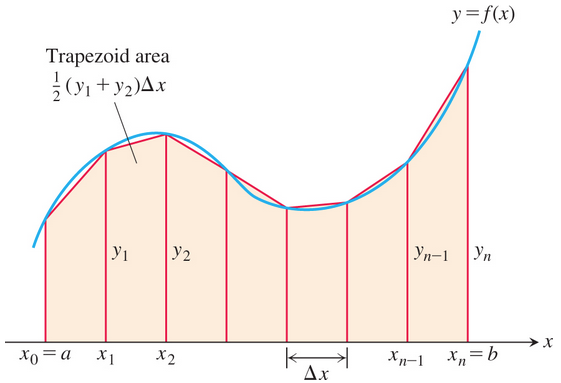
\includegraphics[height=2.5in]{img/trapezoidal_rule}
\end{figure}
\item  Therefore,
\begin{equation*}
\int_a^bf(x)\dee x 
= \sum_{i=1}^n\int_{x_{i-1}}^{x_i} f(x)\dee x
\approx \sum_{i=1}^n\int_{x_{i-1}}^{x_i} p_i(x)\dee x
= \frac{\Delta x}{2}\sum_{i=1}^n\left(y_i+y_{i-1}\right).
\end{equation*}
\end{itemize}
\end{remark}


\newpage

\begin{example}
Use the trapezoidal rule with $n=6$ to estimate $\ln 2$.
\end{example}

\ifdefined\SOLUTION
\SOLUTION[Solution]{
Recall that 
\begin{equation*}
\ln(2) = \int_1^2 \frac{\dee t}{t}. 
\end{equation*}
So, we apply the trapezoidal rule with $f(t)=1/t$, $a = 1$, $b = 2$, and $n = 6$.  
Whence, 
\begin{equation*}
\Delta x = \frac{b-a}{n} = \frac{2-1}{6} = \frac{1}{6},
\end{equation*}
and
\begin{align*}
y_0 &= f(a) = f(1) = 1, \\
y_1 &= f(a+\Delta x) = f(7/6) = 6/7, \\
y_2 &= f(a+2\Delta x) = f(8/6) = 6/8, \\
y_3 &= 6/9, \\
y_4 &= 6/10, \\
y_5 &= 6/11, \\
y_6 &= 6/12 = 1/2.
\end{align*}
Therefore, 
\begin{equation*}
\ln(2) 
\approx \frac{1/6}{2}\left[ 1 + 2(6/7 + 6/8 + 6/9 + 6/10 + 6/11) + 1/2\right] 
= \frac{9631}{13860} \approx 0.694877.
\end{equation*}
}
\else
\fi
\newpage

\begin{remark}
When the second derivative $f''$ is continuous on $[a,b]$, we can use the following theorem to bound the error in the trapezoidal approximation.
\end{remark}

\begin{theorem}
Suppose $f''$ is continuous on $[a,b]$ and $\DS M=\max_{a\le x\le b}|f''(x)|$.
If $E_T$ is the error in the $n$-step  trapezoidal approximation of $\int_a^bf(x)\dee x$, then
\begin{align*}
%|E_M| &\le \frac{M(b-a)^3}{24n^2},\\
|E_T| &\le \frac{M(b-a)^3}{12n^2}.
\end{align*}
\end{theorem}

\begin{example}
Use the above to bound the error in the trapezoidal approximation of $\ln 2$ when $n=6$.
How large must $n$ be to ensure that the error is less than $10^{-6}$?
\end{example}
\ifdefined\SOLUTION
\SOLUTION[Solution]{
Since $\ln(2) = \int_1^2 \frac{\dee t}{t}$, we need to compute the global extrema of $f''(t)$ over the interval $[a,b]$, 
where $f(t)=1/t$ and $[a,b]=[1,2]$.
First, we calculate that
\begin{align*}
f'(t)   &= -t^{-2}, \\
f''(t)  &= 2t^{-3},\\
f'''(t) &= -6t^{-4}.
\end{align*}
It is clear that $f''(t)$ has no critical points on the interval $[1,2]$.
So, we only need to check the endpoints of the interval.
Since
\begin{align*}
|f''(1)| &= 2,\\
|f''(2)| &= 1/4,
\end{align*}
it follows that 
\begin{equation*}
M=\max_{a\le t\le b}|f''(t)| = 2.
\end{equation*}
Therefore, with $n$ steps of the trapezoidal rule, the error $E_T$ satisfies
\begin{equation*}
|E_T| \le \frac{M(b-a)^3}{12n^2} = \frac{2(2-1)^3}{12n^2} = \frac{1}{6n^2}.
\end{equation*}
So, when $n=6$, we have $|E_T| \le 1/6^3 \approx 0.00462963$.
To guarantee $|E_T|<10^{-6}$, we force
\begin{equation*}
|E_T|\le\frac{1}{6n^2}<10^{-6}.
\end{equation*}
Solving the latter inequality for $n$ yields $n >\sqrt{10^6/6} \approx 408.248$.
So, to guarantee $|E_T|<10^{-6}$, we require $n\ge 409$.
}
\else
\fi
\newpage

\begin{remark}\,
\begin{itemize}
\item In some situations, Simpson's approximation achieves ``faster" convergence by using a quadratic interpolation.
\item Just as we need 2 points to determine a line, we need 3 to determine a parabola.
\item As a consequence, we must partition the interval $[a,b]$ into an even number of pieces.
\end{itemize}
\end{remark}

\begin{figure}[H]
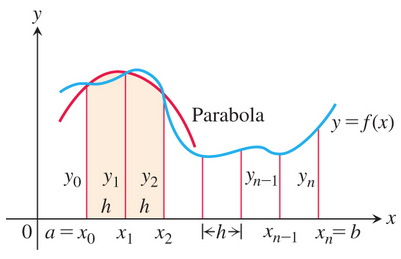
\includegraphics[height=2.5in]{img/simpson_rule}
\end{figure}

\begin{definition}[Simpson's rule]
Let $[a,b]$ be a finite length interval, and let $f$ be continuous on $[a,b]$.
\begin{itemize}
\item Partition the interval $[a,b]$ into $n=2m \ge 2$ (an even number of) equal length pieces
\begin{equation*}
a=x_0 < x_1 <\dots < x_{n-1} < x_n = b,
\end{equation*}
where $\Delta x = x_i - x_{i-1} = \frac{b-a}{n}$ for $i=1,\dots, n$.
\item For $i=0,1,\dots, n$, evaluate $y_i = f(x_i)$.
\end{itemize}
\textbf{Simpson's approximation} is
\begin{equation*}
\begin{split}
\int_a^bf(x)\dee x &\approx \frac{\Delta x}{3}\left[y_0 + 4\sum_{i=0}^{m-1} y_{2i+1} + 2\sum_{i=1}^{m-1} y_{2i} + y_n\right]\\
&= \frac{\Delta x}{3}\Big(y_0 + 4y_1 + 2y_2 + \dots + 2y_{n-2} + 4y_{n-1} + y_n\Big).
\end{split}
\end{equation*}
\end{definition}

\newpage

\begin{example}
Use Simpson's rule with $n=6$ to estimate $\ln 2$.
\end{example}
\ifdefined\SOLUTION
\SOLUTION[Solution]{
Recall that 
\begin{equation*}
\ln(2) = \int_1^2 \frac{\dee t}{t}. 
\end{equation*}
So, we apply Simpson's rule with $f(t)=1/t$, $a = 1$, $b = 2$, and $n = 6$.  
Whence, 
\begin{equation*}
\Delta x = \frac{b-a}{n} = \frac{2-1}{6} = \frac{1}{6},
\end{equation*}
and
\begin{align*}
y_0 &= f(a) = f(1) = 1, \\
y_1 &= f(a+\Delta x) = f(7/6) = 6/7, \\
y_2 &= f(a+2\Delta x) = f(8/6) = 6/8, \\
y_3 &= 6/9, \\
y_4 &= 6/10, \\
y_5 &= 6/11, \\
y_6 &= 6/12 = 1/2.
\end{align*}
Therefore, 
\begin{align*}
\ln{2} 
&\approx \frac{\Delta x}{3}\left[ y_0 + 4(y_1 + y_3 + y_5) + 2(y_2 + y_4) + y_6 \right] \\
&= \frac{1/6}{3}\left[ 1 + 4(6/7 + 6/9 + 6/11) + 2(6/8 + 6/10) + 1/2 \right] \\
&= \frac{14411}{20790} \\
& \approx 0.69317. 
\end{align*}
}
\else
\fi

\newpage

\begin{theorem}
Suppose $f^{(4)}$ is continuous on $[a,b]$ and $\DS M=\max_{a\le x\le b}|f^{(4)}(x)|$.
If $E_S$ is the $n$-step error in Simpson's approximation of $\int_a^bf(x)\dee x$, then
\begin{equation*}
|E_S| \le \frac{M(b-a)^5}{180n^4}.
\end{equation*}
\end{theorem}



\begin{example}
Use the above to bound the error in Simpson's approximation of $\ln 2$ when $n=6$.
How large must $n$ be to ensure that the error is less than $10^{-6}$?
\end{example}
\ifdefined\SOLUTION
\SOLUTION[Solution]{
This time we need to compute
\begin{equation*}
M = \max_{a\le t\le b}|f^{(4)}(t)|,
\end{equation*}
where again $f(t)=1/t$ and $[a,b]=[1,2]$.
Using our calc I skills, we easily show that
\begin{equation*}
M = \max_{1\le t\le 2}|24t^{-5}| = 24.
\end{equation*}
Therefore, with $n$ steps of Simpson's rule, we have
\begin{equation*}
\left| E_S\right| \leq \frac{M(b-a)^5}{180n^4} = \frac{24}{180n^4}.
\end{equation*}
When $n=6$, this means that $|E_S|\le \frac{1}{9720}\approx 0.00010$.
To ensure $|E_S| < 10^{-6},$ we force 
\begin{equation*}
|E_S|\le \frac{24}{180n^4} < 10^{-6}.
\end{equation*}
Solving, we find that the smallest even integer satisfying the inequality is $n=20$.
}
\else
\fi

\setcounter{equation}{0}

%!TEX root =  main.tex

\lectureheader{162}{Calculus II}{Improper integrals}{\textit{Thomas' Calculus} \textsection 8.8}

\begin{remark}\,
\begin{itemize}
\item When we defined the definite integral $\DS\int_a^bf(x)\dee x$ as a limit of Riemann sums, we assumed that $[a,b]$ was a finite length interval and that $f$ was continuous on $[a,b]$.
\item Occasionally, it is possible to somewhat relax these two conditions.
Such integrals are referred to as \textbf{improper integrals}.
\end{itemize}
\end{remark}

\begin{definition}[Improper integrals of type I]\,
\begin{itemize}
\item If $\DS\int_a^tf(x)\dee x$ exists for every $t\ge a$, then we define
\begin{equation*}
\int_a^\infty f(x)\dee x = \lim_{t\to\infty}\int_a^t f(x)\dee x
\end{equation*}
provided that the limit exists.
\item If $\DS\int_t^bf(x)\dee x$ exists for every $t\le b$, then we define
\begin{equation*}
\int_{-\infty}^b f(x)\dee x = \lim_{t\to-\infty}\int_t^b f(x)\dee x
\end{equation*}
provided that the limit exists.
\end{itemize}
We say that the integrals above are \textbf{convergent} when they exist; otherwise we say that they are \textbf{divergent}.
\begin{itemize}
\item If there is a real number $c$ so that both $\DS\int_c^\infty f(x)\dee x$ and $\DS\int_{-\infty}^cf(x)\dee x$ are both convergent, then we define
\begin{equation*}
\int_{-\infty}^\infty f(x)\dee x = \int_{-\infty}^cf(x)\dee x + \int_c^\infty f(x)\dee x.
\end{equation*}
\end{itemize}
\end{definition}

\newpage

\begin{example}
What is the area of the region under the curve $y=\DS\frac{\ln x}{x^2}$ over the interval $[1,\infty)$?
\end{example}

\newpage

\begin{theorem}
Let $p\in\R$.
The integral $\DS\int_1^\infty\frac{\dee x}{x^p}$ converges if and only if $p>1$.
\end{theorem}
\begin{proof}\,

\vspace{5in}
\end{proof}

\newpage

\begin{example}
Evaluate $\DS\int_{-\infty}^\infty\frac{\dee x}{1+x^2}$.
\end{example}

\newpage

\begin{theorem}[Test for divergence]
If $\int_a^\infty f(x)\dee x$ converges, then $f(x)\to 0$ as $x\to\infty$.
\end{theorem}
\begin{remark}
In practice, we use the test for divergence in the form of its contrapositive, viz.,
\begin{equation*}
\lim_{x\to\infty} f(x)\ne 0 \implies \int_a^\infty f(x)\dee x \text{ diverges}.
\end{equation*}
\end{remark}

\begin{example}
Show that $\DS\int_1^\infty \left(1-\frac{1}{x}\right)^{x}\dee x$ diverges.
\end{example}

\newpage

\begin{definition}[Improper integrals of type II]\,
\begin{itemize}
\item If $f$ is continuous on $[a,b)$ but discontinuous at $x=b$, then we define
\begin{equation*}
\int_a^b f(x)\dee x = \lim_{t\to b^-}\int_a^t f(x)\dee x
\end{equation*}
provided that the limit exists.
\item If $f$ is continuous on $(a,b]$ but discontinuous at $x=a$, then we define
\begin{equation*}
\int_{a}^b f(x)\dee x = \lim_{t\to a^+}\int_t^b f(x)\dee x
\end{equation*}
provided that the limit exists.
\end{itemize}
We say that the integrals above are \textbf{convergent} when they exist; otherwise we say that they are \textbf{divergent}.
\begin{itemize}
\item If $f$ is continuous on $[a,b]$ except for a discontinuity at $c\in (a,b)$, then we define
\begin{equation*}
\int_{a}^b f(x)\dee x = \int_{a}^cf(x)\dee x + \int_c^b f(x)\dee x.
\end{equation*}
\end{itemize}
\end{definition}

\begin{example}
Determine $\DS\int_2^5\frac{\dee x}{\sqrt{x-2}}$.
\end{example}

\newpage

\begin{example}
Calculate $\DS\int_0^{\pi/2}\sec x\dee x$.
\end{example}
\vfill

\begin{example}
Evaluate $\DS\int_0^3\frac{\dee x}{x-1}$.
\end{example}
\vfill

\newpage

\begin{theorem}[Direct comparison test for integrals]
Suppose that $f$ and $g$ are continuous functions on the interval $[a,\infty)$.
\begin{enumerate}
\item If $0\le f(x)\le g(x)$ for all $x\ge a$ and $\int_a^\infty g(x)\dee x$ converges, then $\int_a^\infty f(x)\dee x$ also converges.
\item If $0\le g(x)\le f(x)$ for all $x\ge a$ and $\int_a^\infty g(x)\dee x$ diverges, then $\int_a^\infty f(x)\dee x$ also diverges.
\end{enumerate}
\end{theorem}
\begin{proof}\,

\vspace{5in}
\end{proof}

\newpage


\begin{example}
Determine if $\DS\int_0^\infty \E^{-x^2}\dee x$ converges or diverges.
\end{example}

\newpage

\begin{remark}
The idea of the direct comparison test can also be applied to improper integrals of type II.
\end{remark}

\begin{example}
Determine if $\DS\int_0^{\pi/2}\frac{\cos x}{\sqrt x}\dee x$ converges or diverges.
\end{example}

\newpage

\begin{remark}\,
\begin{itemize}
\item The test for divergence tells us that if $\int_a^\infty f(x)\dee x$ is going to have a chance at convergence, then we must have $f(x)\to 0$ as $x\to\infty$.
\item The difference between convergence and divergence for the integral is ``how fast" $f(x)$ tends toward zero.
\item The comparison tests are about determining convergence by comparing the relative sizes of the integrands.
\item For the direct comparison test we have to be careful to get the inequalities correct for \textit{all sufficiently large} $x$.
\item The limit comparison tests allows for ``cruder" comparison using limits.
\end{itemize}
\end{remark}

\begin{theorem}[Limit comparison test for integrals]
Suppose that $f$ and $g$ are positive and continuous on $[a,\infty)$.
\begin{enumerate}
\item If $f(x) \asymp g(x)$ as $x\to\infty$ (in particular, if $\DS\lim_{x\to\infty}\frac{f(x)}{g(x)}=L>0$), 
then $\int_a^\infty f(x)\dee x$ and $\int_a^\infty g(x)\dee x$ both converge or both diverge.
\item If $f(x) \lll g(x)$ as $x\to\infty$ (i.e., if $\DS\lim_{x\to\infty}\frac{f(x)}{g(x)}=0$) and $\int_a^\infty g(x)\dee x$ converges, 
then $\int_a^\infty f(x)\dee x$ converges.
\item If $f(x) \ggg g(x)$ as $x\to\infty$ (i.e., if $\DS\lim_{x\to\infty}\frac{f(x)}{g(x)}=\infty$) and $\int_a^\infty g(x)\dee x$ diverges, 
then $\int_a^\infty f(x)\dee x$ diverges.
\end{enumerate}
\end{theorem}

\begin{example}
Determine if $\DS\int_1^\infty\frac{1-\E^{-x}}{x}\dee x$ converges or diverges.
\end{example}

\newpage

\begin{example}
Determine if $\DS\int_4^\infty\frac{x\dee x}{(3x^2+4)^{5/2}}$ converges or diverges.
\end{example}

\setcounter{equation}{0}


%!TEX root =  main.tex

\lectureheader{162}{Calculus II}{Infinite sequences}{\textit{Thomas' Calculus} \textsection 10.1}

\begin{definition}\,
\begin{itemize}
\item A \textbf{sequence} is a function whose domain is a subset of $\Z$ (the set of whole numbers).
\item The values of the function are called \textbf{terms} of the sequence.
\item An \textbf{infinite sequence} is a sequence whose domain is infinite.
\end{itemize}
\end{definition}

\begin{remark}
In practice, we view a sequence as an ordered list of real numbers
\begin{equation*}
a_1, a_2, a_3,\dots.
\end{equation*}
In calculus, we are mostly interested in sequences that can be described by simple rules/formulas or by recursion.
\end{remark}

\begin{definition}
Let $\{a_n\}$ be an infinite sequence, and let $L$ be a real number.
\begin{itemize}
\item We say that $\{a_n\}$ \textbf{converges} to $L$, and we write $a_n\to L \text{ as } n\to\infty$ or
\begin{equation*}
\lim_{n\to\infty}a_n = L,
\end{equation*}
if for every $\epsilon>0$, there is an integer $N$ so that
\begin{equation*}
n>N \implies |a_n - L|<\epsilon.
\end{equation*}
\item If $\{a_n\}$ does not converge to any real number $L$, then we say that $\{a_n\}$ \textbf{diverges}.
\end{itemize}
\end{definition}

\begin{remark}\,
\begin{itemize}
\item For many applications, the notation $\DS\lim_{n\to\infty} a_n= L$ makes the interesting part of the limit implicit.
\item Often (though not always) it is the interplay between the $\epsilon$ and the $N$ in the definition that is truly interesting.
\item Imagine a sequence as list of approximate answers to an interesting question (e.g., what really is $\ln(2)$?).
\item We should think of the $\epsilon$ as an acceptable ``error tolerance" that is subject to change depending on the day-to-day whims of our customer (or zany math prof).
\item The only thing the customer is not allowed to ask for is zero error.  Any $\epsilon>0$ is allowed.
\item We should think of the $N$ as the ``cutoff" past which all approximations are guaranteed to be within requirements (i.e., have acceptable errors).
\item To say $\DS\lim_{n\to\infty} a_n= L$, is to say that no matter how unreasonably small we are asked to get the errors, we can always ``win the game" of finding a finite cutoff $N$ so that if we ``turn $n$ up past $N$" the error is guaranteed to be within tolerance.
\end{itemize}
\end{remark}

\newpage

\begin{example}
Let $T_n$ denote the $n$-step trapezoidal approximation to $\ln 2 = \int_1^2\frac{\dee t}{t}$ for $n\ge 1$.
Then
\begin{equation*}
T_1 = \frac{3}{2},\quad
T_2 = \frac{13}{6},\quad
T_3 =\frac{57}{20},\quad
T_4=\frac{743}{210},\quad
T_5 = \frac{2131}{504},\quad \dots.
\end{equation*}
The trapezoidal approximation theorem tells us that
\begin{equation*}
\left| T_n - \ln 2\right| \le \frac{1}{6n^2}.
\end{equation*}
Use this fact to show that $T_n\to \ln 2$ as $n\to\infty$.
\end{example}

\newpage

\begin{definition}
Let $\{a_n\}$ be an infinite sequence, and let $L$ be a real number.
\begin{itemize}
\item We say that $\{a_n\}$ \textbf{diverges} to $\infty$, and we write $a_n\to\infty$ as $n\to\infty$ or
\begin{equation*}
\lim_{n\to\infty}a_n = \infty
\end{equation*}
if for every $M>0$, there is an integer $N$ so that
\begin{equation*}
n>N\implies a_n>M.
\end{equation*}
\item We say that $\{a_n\}$ \textbf{diverges} to $-\infty$, and we write $a_n\to -\infty$ as $n\to\infty$ or
\begin{equation*}
\lim_{n\to\infty}a_n = -\infty
\end{equation*}
if for every $M<0$, there is an integer $N$ so that
\begin{equation*}
n>N\implies a_n<M.
\end{equation*}
\end{itemize}
\end{definition}

\begin{example}
If $n$ is a nonnegative integer, then $n$-\textbf{factorial} is 
\begin{equation*}
n! = \prod_{j=0}^{n-1}\left(n-j\right).
\end{equation*}
List the first 5 terms, and then determine whether the sequence converges or diverges.
\end{example}

\newpage

\begin{theorem}
For all integers $n\ge 1$, 
\begin{equation*}
\E\left(\frac{n}{\E}\right)^n\le n!\le n^{n-1}.
\end{equation*}
\end{theorem}
\begin{remark}
Stirling is famous for proving a much more precise relationship, viz., for every $\epsilon>0$, there is an $N>0$ so that
\begin{equation*}
(1-\epsilon) \sqrt{2\pi n}\left(\frac{n}{\E}\right)^n\le n!\le (1+\epsilon) \sqrt{2\pi n}\left(\frac{n}{\E}\right)^n
\end{equation*}
for all $n>N$.
\end{remark}
\begin{proof}\,

\vspace{6in}
\end{proof}



\newpage

\begin{remark}\,
\begin{itemize}
\item Sequences are discrete (not continuous) and so they can't have derivatives.
\item That's bad news for L'H\^opital's rule, but the following theorem tells us that if our sequence is the restriction of a function to integer inputs, then pretty much everything that we're used doing with limits at $\infty$ for functions still works including L'H\^opital's rule (when it applies).
\end{itemize}
\end{remark}

\begin{theorem}
Let $\{a_n\}$ be an infinite sequence, and let $f(x)$ be a function that is defined for all sufficiently large $x$.
If $f(n) = a_n$ for all sufficiently large integers $n$, then
\begin{equation*}
\lim_{x\to\infty}f(x) = L \implies \lim_{n\to\infty} a_n=  L.
\end{equation*}
\end{theorem}

\begin{example}
Compute the following.
\begin{enumerate}
\item $\DS\lim_{n\to\infty}\frac{n}{n+1}$
\vfill
\item $\DS\lim_{n\to\infty}\frac{\ln n}{n}$
\vfill
\item $\DS\lim_{n\to\infty}\left(\frac{n+1}{n-1}\right)^n$
\vfill
\end{enumerate}
\end{example}


\newpage

\begin{theorem}
If $\{a_n\}$ is a sequence of real numbers and $\DS\lim_{n\to\infty}|a_n|=0$, then $\DS\lim_{n\to\infty}a_n=0$.
\end{theorem}

\begin{example}
Show that the sequence $\{a_n\}$ whose terms are defined by 
\begin{equation*}
a_n = \frac{(-1)^n}{n}\quad (n\ge 1)
\end{equation*}
converges.
\end{example}

\vfill


\begin{example}
Does the sequence $\{a_n\}$ whose terms are defined by
\begin{equation*}
a_n=(-1)^n\quad (n\ge 0)
\end{equation*}
converge or diverge?
\end{example}

\vfill

\newpage

\begin{theorem}[Squeeze/sandwich theorem]
Let $\{a_n\}$, $\{b_n\}$, and $\{c_n\}$ be sequences of real numbers.
If $a_n\le b_n\le c_n$ for all $n$ sufficient large, then
\begin{equation*}
\lim_{n\to\infty}a_n = L = \lim_{n\to\infty}c_n \implies \lim_{n\to\infty}b_n= L.
\end{equation*}
\end{theorem}

\begin{example}
Determine $\DS\lim_{n\to\infty}\frac{\cos n}{n}$.
\end{example}
\vfill

\begin{example}
Determine if the sequence $\DS a_n=\frac{n!}{n^n}$ converges.
\end{example}
\vfill

\newpage

\begin{example}
For what values of $x$ is the sequence $a_n=x^n$ convergent?
\end{example}
\vfill

\newpage

\begin{theorem}
For every (fixed) $x\in\R$,
\begin{equation*}
\lim_{n\to\infty}\frac{x^n}{n!} = 0.
\end{equation*}
\end{theorem}
\begin{proof}\,

\vspace{6in}
\end{proof}

\begin{remark}
It is sometimes helpful to think about the above theorem in the following equivalent forms.
\begin{enumerate}
\item If $x\in\R$, then $x^n\lll n!$ as $n\to\infty$.
\item If $x\in\R$, then for every $\epsilon>0$, there is an $N>0$ so that
\begin{equation*}
n>N\implies |x|^n \le\epsilon n!.
\end{equation*}
\end{enumerate}
\end{remark}

\newpage

\begin{definition}
Let $\{a_n\}$ be a sequence of real numbers.
\begin{itemize}
\item We say that $\{a_n\}$ is \textbf{bounded above} if there is a real number $M$ so that $a_n\le M$ for all $n$, in which case we say that $M$ is an \textbf{upper bound} for $\{a_n\}$.
\item If $L$ is an upper bound for $\{a_n\}$ and no smaller number is also an upper bound for $\{a_n\}$, then we say that $L$ is the \textbf{least upper bound} for $\{a_n\}$.
\item We say that $\{a_n\}$ is \textbf{bounded below} if there is a real number $m$ so that $a_n\ge m$ for all $n$, in which case we say that $m$ is an \textbf{lower bound} for $\{a_n\}$.
\item If $G$ is a lower bound for $\{a_n\}$ and no larger number is also a lower bound for $\{a_n\}$, then we say that $G$ is the \textbf{greatest lower bound} for $\{a_n\}$.
\item We say that $\{a_n\}$ is \textbf{bounded} if it is bounded above and below.
If $\{a_n\}$ is not bounded, we say that it is \textbf{unbounded}.
\end{itemize}
\end{definition}

\begin{example}
Determine if the following sequences are bounded.
\begin{enumerate}
\item $a_n = n\quad (n\ge 0)$
\vfill
\item $a_n=(-1)^n n\quad (n\ge 0)$
\vfill
\item $a_n =\DS \frac{n}{n+1}\quad (n\ge 0)$
\vfill
\end{enumerate}
\end{example}


\newpage

\begin{definition}
Let $\{a_n\}$ be a sequence of real numbers.
\begin{itemize}
\item We say that the sequence is \textbf{nondecreasing} if $a_n\le a_{n+1}$ for all $n$.
\item We say that the sequence is \textbf{nonincreasing} if $a_n\ge a_{n+1}$ for all $n$.
\item If the sequence is nondecreasing or nonincreasing, then we say that it is \textbf{monotonic}.
\end{itemize}
\end{definition}

\begin{example}
Determine whether each sequence below is monotonic
\begin{enumerate}
\item $a_n=n\quad (n\ge 0)$
\vfill
\item $\DS a_n=\frac{n}{n+1}\quad (n\ge 0)$
\vfill
\item $a_n=3\quad (n\ge 0)$
\vfill
\item $a_n=(-1)^n\quad (n\ge 0)$
\vfill
\end{enumerate}
\end{example}

\newpage

\begin{theorem}[Monotonic sequence theorem]
Let $\{a_n\}$ be a monotonic sequence.  
Then
\begin{equation*}
\{a_n\} \text{ is bounded} \iff \{a_n\} \text{ is convergent}.
\end{equation*}
\end{theorem}
\begin{proof}[Proof when $\{a_n\}$ is nondecreasing ($\implies$)]\,

\vspace{7in}
\end{proof}

\setcounter{equation}{0}

%!TEX root =  main.tex

\lectureheader{162}{Calculus II}{Infinite series}{\textit{Thomas' Calculus} \textsection 10.2}

\begin{definition}\,
Let $\{a_n\}_{n=0}^\infty$ be a sequence of real numbers.
\begin{itemize}
\item The sequence of \textbf{partial sums} is 
\begin{equation*}
s_n = \sum_{k=0}^na_k.
\end{equation*}
\item The limit 
\begin{equation*}
\sum_{k=0}^\infty a_k = \lim_{n\to\infty}s_n
\end{equation*}
is called an \textbf{infinite series}.
\item We say that the series \textbf{converges} if the above limit exists, otherwise we say that the series \textbf{diverges}.
\end{itemize}
\end{definition}
\begin{remark}\,
\begin{itemize}
\item The thing that makes series more difficult than sequences is the fact that the sequence of partial terms is given to us as the sum of an ever-increasing number of terms.
\item To evaluate a series, it is helpful if we can express the partial sums in ``closed form."
\item We have  very few ``tricks" for evaluating the sum of an infinite series.
\item If the sequence of partial sums $s_n$ can be rewritten as
\begin{equation*}
s_n = \sum_{k=0}^n a_k = \sum_{k=0}^n \big(b_{k+1} - b_k\big),
\end{equation*}
then we say that the series is \textbf{telescoping} and
\begin{equation*}
\begin{split}
s_n &= \sum_{k=0}^n \big(b_{k+1} - b_k\big)\\
& = (b_1 - b_0) + (b_2 - b_1) + \dots + (b_{n+1} - b_n)\\
& = b_{n+1} - b_0.
\end{split}
\end{equation*}
\end{itemize}
\end{remark}

\newpage

\begin{example}
Compute the first 3 partial sums of the series $\DS\sum_{k=0}^\infty \frac{1}{(k+1)(k+2)}$.
Then determine if the series converges or diverges.
\end{example}

\newpage

\begin{definition}
A \textbf{geometric series} is a series of the form $\DS\sum_{n=0}^\infty ar^n$, where $a$ and $r$ are fixed real numbers.
\end{definition}

\begin{theorem}[Geometric series theorem]
Let $a,r\in\R$.
The series $\DS\sum_{n=0}^\infty ar^n$ converges if and only if $|r|<1$, in which case
\begin{equation*}
\sum_{n=0}^\infty ar^n = \frac{a}{1-r}.
\end{equation*}
\end{theorem}
\begin{proof}\,

\vspace{6in}
\end{proof}

\newpage 

\begin{example}
Evaluate $\DS\sum_{n=0}^\infty\frac{(-1)^n5}{4^n}$ if possible.
\end{example}

\newpage

\begin{theorem}[Test for divergence]
If $\DS\sum a_n$ converges, then $a_n\to 0$ as $n\to\infty$.
\end{theorem}
\begin{remark}
In practice, we use this theorem in the form of its contrapositive, viz.,
\begin{equation*}
\lim_{n\to\infty} a_n\ne 0 \implies \sum a_n \text{ diverges}.
\end{equation*}
\end{remark}
\begin{proof}\,

\vspace{3in}
\end{proof}
\begin{example}
Explain why the series below diverge.
\begin{enumerate}
\item $\DS\sum_{n=1}^\infty \frac{n+1}{n}$
\vfill
\item $\DS\sum_{n=0}^\infty (-1)^n$
\vfill
\end{enumerate}
\end{example}

\newpage

\begin{theorem}
If $\sum a_n$ and $\sum b_n$ both converge and $k\in\R$, then
\begin{enumerate}
\item $\sum \big(a_n\pm b_n\big) = \sum a_n \pm \sum b_n$,
\item $\sum ka_n = k\sum a_n$.
\end{enumerate}
\end{theorem}

\begin{example}
Evaluate the series below.
\begin{enumerate}
\item $\DS\sum_{n=1}^\infty \frac{3^{n-1} - 1}{6^{n-1}}$
\vfill
\item $\DS\sum_{n=1}^\infty \frac{4}{2^n}$
\vfill
\end{enumerate}
\end{example}

\setcounter{equation}{0}

%!TEX root =  main.tex
\setcounter{chapter}{10}
\setcounter{section}{3}
\setcounter{theorem}{0}
\setcounter{equation}{0}

\lectureheader{162}{Calculus II}{The integral test}{\textit{Thomas' Calculus}  \thesection}

\begin{lemma}
If $f$ is a nonnegative, continuous, and decreasing function on the interval $[n, n+1]$, then
\begin{equation*}
0\le f(n) - \int_n^{n+1}f(x)\dee x < f(n) - f(n+1).
\end{equation*}
\end{lemma}

\begin{figure}[h]
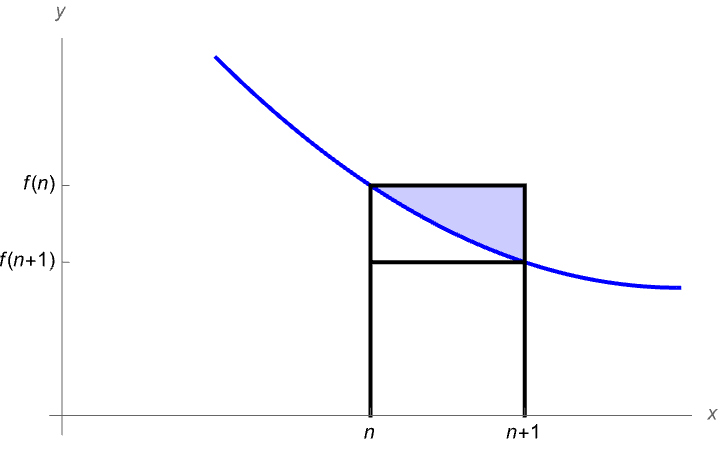
\includegraphics[width=5in]{img/series_integral_diff}
\end{figure}

\newpage

\begin{theorem}[Integral test]
Suppose that $f$ is nonnegative, continuous, and decreasing for all $x\ge k$.
Then
\begin{equation*}
\sum_{n=k}^\infty f(n) \text{ converges }\iff \int_k^\infty f(x)\dee x \text{ converges}.
\end{equation*}
\end{theorem}
\ifdefined\SOLUTION
\SOLUTION[Proof]{
%The idea is ``approximate" the $N$th partial sum
%\begin{equation*}
%S_N = \sum_{n=k}^Nf(n)
%\end{equation*}
%by the integral $\DS\int_k^{N+1}f(x)\dee x$. 
For $N\ge k$, we let
\begin{equation*}
\begin{split}
E_N 
&= S_N - \int_k^{N+1}f(x)\dee x\\
&= \sum_{n=k}^Nf(n) - \int_k^{N+1}f(x)\dee x\\
&= \sum_{n=k}^Nf(n) - \sum_{n=k}^N\int_{n}^{n+1}f(x)\dee x\\
&= \sum_{n=k}^N\left(f(n) - \int_n^{n+1}f(x)\dee x\right).
\end{split}
\end{equation*}
Since the lemma tell us that
\begin{equation*}
0\le f(n) - \int_n^{n+1}f(x)\dee x,
\end{equation*}
it follows that $E_N$ is a monotonic nondecreasing sequence which is bounded below by $0$.
Since the lemma also tells us that
\begin{equation*}
f(n) - \int_n^{n+1}f(x)\dee x < f(n) - f(n+1),
\end{equation*}
it follows that
\begin{equation*}
E_N < \sum_{n=k}^N\Bigg(f(n) - f(n+1)\Bigg) = f(k) - f(N+1) \le f(k),
\end{equation*}
i.e., $E_N$ is bounded above by $f(k)$.
By the monotonic sequence theorem, $E_N\to L$ as $N\to\infty$ for some (finite) nonnegative real number $L<f(k)$.
Therefore, if $\DS\sum_{n=k}^\infty f(n)$ converges, then
\begin{equation*}
\int_k^\infty f(x)\dee x
=\lim_{N\to\infty}\int_k^{N+1}f(x)\dee x
=\lim_{N\to\infty}\left(S_N-E_N\right)
=\sum_{n=k}^\infty f(n) - L.
\end{equation*}
In particular, the improper integral also converges.
Similarly, if $\DS\int_k^\infty f(x)\dee x$ converges, then
\begin{equation*}
\sum_{n=k}^\infty f(n) = \int_k^\infty f(x)\dee x + L.
\end{equation*}
}
\else
\begin{proof}\,

\vspace{6in}
\end{proof}
\fi

\newpage

\begin{definition}
A $p$\textbf{-series} is a series of the form
\begin{equation*}
\sum_{n=1}^\infty \frac{1}{n^p},
\end{equation*}
where $p\in\R$.
The special case when $p=1$ is called the \textbf{harmonic series}.
\end{definition}

\begin{theorem}[$p$-series test]
The $p$-series converges if and only if $p>1$.
In particular, the harmonic series diverges.
\end{theorem}

\ifdefined\SOLUTION
\SOLUTION[Proof]{
Let $p\in\R$.
\begin{equation*}
\lim_{n\to\infty} \frac{1}{n^p} = 
\begin{cases}
\infty &\text{if } p<0,\\
1 & \text{if } p=0.
\end{cases}
\end{equation*}
Therefore, the $p$-series diverges by the test for divergence if $p\le 0$.
Suppose then that $p>0$.
Then $f(x) = 1/x^p$ is nonegative, continuous, and decreasing for all $x\ge 1$.
By the integral test, $\sum_{n=1}^\infty\frac{1}{n^p}$ converges if and only if $\int_1^\infty\frac{\dee x}{x^p}$ converges.
By the $p$-test for integrals $\int_1^\infty\frac{\dee x}{x^p}$ converges if and only if $p>1$.
}
\else
\begin{proof}\,

\vspace{3.25in}
\end{proof}
\fi

\vfill

\begin{remark}[Even simple series are often hard!]\,
\begin{itemize}
\item The proof of the integral test tells us that if $f$ is nonnegative, continuous, and decreasing for all $x\ge k$ and the integral exists, then
\begin{equation*}
%\sum_{n=k}^N f(n) \asymp \int_k^Nf(x)\dee x\quad\text{ as } N\to\infty.
0\le \sum_{n=k}^\infty f(n) - \int_k^\infty f(x)\dee x < f(k).
\end{equation*}
\item It does \underline{not} tell us that the infinite series and the improper integral are equal.  
It tells us that if $f(k)$ is small, then they are good approximations of one another, but most likely they are different.
\item Even though we know how to evaluate the integral $\int_1^\infty\frac{\dee x}{x^p}$ exactly when it exists,
we only know the value of the series $\sum_{n=1}^\infty\frac{1}{n^p}$ for even integers $p\ge 2$.
\item For example, Euler showed
\begin{equation*}
\sum_{n=1}^\infty\frac{1}{n^2} = \frac{\pi^2}{6}.
\end{equation*}
%\item Euler also showed that the divergence of the harmonic series can be used to give a novel proof that there are infinitely many prime numbers.
%\item Riemann would later change the real variable $p$ to a complex variable $s$, and show how the series is connected to a much deeper theory of prime numbers.
\end{itemize}
\end{remark}

\newpage

\begin{example}
Determine whether the following converge or diverge.
\begin{enumerate}
\item $\DS\sum_{n=1}^\infty\frac{1}{n^2+1}$
\ifdefined\SOLUTION
\SOLUTION[Solution]{
Note that $f(x)=1/(x^2+1)$ is positive, continuous, and decreasing for $x\ge 1$.
Therefore, since 
\begin{equation*}
\begin{split}
\int_1^\infty \frac{\dee x}{x^2 + 1} 
&=\lim_{x\to\infty} \int_1^t \frac{\dee x}{x^2 + 1} 
=\lim_{t \to \infty} \arctan{(t)} \Big|_1^t\\
&=\lim_{t\to\infty} \left[ \arctan{t} - \arctan{1}\right] 
=\frac{\pi}{2} - \frac{\pi}{4} = \frac{\pi}{4},
\end{split}
\end{equation*}
it follows that the series $\DS\sum_{n=1}^\infty\frac{1}{n^2+1}$ converges by the integral test.
}
\fi
\vfill
\item $\DS\sum_{n=1}^\infty n\E^{-n^2}$
\ifdefined\SOLUTION
\SOLUTION[Solution]{
Note that $f(x) = x\E^{-x^2}$ is positive, continuous, and decreasing for $x\ge 1$.
Also
\begin{equation*}
\begin{split}
\int_1^\infty x\E^{-x^2}\dee x 
&=\lim_{t\to\infty} \int_1^t x\E^{-x^2} \dee x
=\lim_{t\to\infty} -\frac{1}{2}\int_1^t (-2)x\E^{-x^2} \dee x\\
&=\lim_{t\to\infty} -\frac{1}{2}\E^{-x^2}\Big|_1^t
=\lim_{t\to\infty} \left( \frac{1}{2}\E^{-1} - \frac{1}{2}\E^{-t^2} \right) = \frac{1}{2\E}.
\end{split}
\end{equation*}
Therefore, $\DS\sum_{n = 1}^\infty n\E^{-n^2}$ converges by the integral test.
}
\fi
\vfill
\item $\DS\sum_{n=1}^\infty\frac{1}{2^{\ln n}}$
\ifdefined\SOLUTION
\SOLUTION[Solution]{
Observe that
\begin{equation*}
2^{\ln{(n)}} = \exp \left(\ln{\left(2^{\ln{n}} \right)}\right) = \exp \left( (\ln n)(\ln 2) \right) = \left(\E^{\ln n}\right)^{\ln(2)} = n^{\ln 2}.
\end{equation*}
Therefore,
\begin{equation*}
\sum_{n = 1}^\infty \frac{1}{2^{\ln n}} = \sum_{n = 1}^\infty \frac{1}{n^{\ln 2}}
\end{equation*}
diverges by the $p$-test with $p = \ln (2) < 1$.
}
\fi
\vfill
\end{enumerate}
\end{example}

\newpage

\begin{remark}\,
\begin{itemize}
\item Even when the integral and series both diverge, the proof of the integral test has more to say.
\item Recall from the proof that if $f$ is nonnegative, continuous, and decreasing for all $x\ge k$, then
\begin{equation*}
\left|\sum_{n=k}^N f(n) - \int_k^{N+1} f(x)\dee x\right| < f(k)
\end{equation*}
for all finite $N\ge k$.
\item This means that in the case of divergence, the integral and the sum are asymptotic to one another, i.e., 
\begin{equation*}
S_N = \sum_{n=k}^N f(n) \sim \int_k^{N+1}f(x)\dee x \text{ as } N\to\infty.
\end{equation*}
\item For example, the $N$th harmonic number
\begin{equation*}
H_N = \sum_{n=1}^N\frac{1}{n} \sim \int_1^{N+1}\frac{\dee x}{x} = \ln(N+1) \text{ as }N\to\infty.
\end{equation*}
\end{itemize}
\end{remark}

\vfill

\begin{definition}
The \textbf{Euler--Mascheroni constant} $\gamma$ is defined by 
\begin{equation*}
\gamma = \lim_{N\to \infty}\left(\sum_{n=1}^N\frac{1}{n} - \ln(N+1)\right)\approx 0.57721566.
\end{equation*}
\end{definition}

\vfill

\begin{remark}\,
\begin{itemize}
\item The Euler--Mascheroni constant is one of the most mysterious numbers in mathematics.
\item It shows up all over the place in seemingly disparate areas of mathematics, and to this day we don't even know whether it is rational or irrational.
\item It is also your professor's favorite number.
\item Our proof of the integral test is essentially just a generalization of Euler's proof that $\gamma$ exists.
\end{itemize}
\end{remark}

\newpage

\begin{remark}\,
\begin{itemize}
\item If we know that a series $\DS\sum_{n=0}^\infty a_n$ converges, 
then we can approximate its sum by the $N$th partial sum, i.e., 
\begin{equation*}
\sum_{n=0}^\infty a_n \approx S_N = \sum_{n=0}^N a_n
\end{equation*}
when $N$ is large.
\item The (signed) error in this approximation 
\begin{equation*}
R_N = \sum_{n=0}^\infty a_n - S_N = \sum_{n=N+1}^\infty a_n
\end{equation*}
is called the \textbf{$N$-th remainder} (or \textbf{tail of the series}).
%\item An infinite series converges if and only if one of its tails converges.
%\item This is because 
%\begin{equation*}
%\sum_{n=k}^\infty a_n = \sum_{n=k}^N a_n + \sum_{n=N+1}^\infty a_n = S_N + R_N
%\end{equation*}
%and $S_N$ is just the sum of finitely many real numbers.
%\item So, if we just want to know if the full series converges or diverges, it doesn't matter where we start $n$.
\end{itemize}
\end{remark}

\begin{theorem}[Integral test estimation theorem]
Suppose that $f$ is nonnegative, continuous, and decreasing for all $x\ge N$, and let $a_n=f(n)$.
If $\DS\sum_{n=0}^\infty f(n)$ converges, then 
\begin{equation*}
0\le  \int_{N+1}^\infty f(x)\dee x\le R_N\le \int_{N}^\infty f(x)\dee x.
\end{equation*}
\end{theorem}
\vfill

\begin{remark}
Because the integral test estimation theorem gives a nonnegative lower bound on the $N$th remainder, we can use it to improve our $N$th partial sum approximation.
\end{remark}

\begin{corollary}
Suppose that $f$ is nonnegative, continuous, and decreasing for all $x\ge N$.
If $\DS\sum_{n=0}^\infty f(n)$ converges, then 
\begin{equation*}
\sum_{n=0}^Nf(n) +  \int_{N+1}^\infty f(x)\dee x\le \sum_{n=0}^\infty f(n)\le \sum_{n=0}^Nf(n) +  \int_{N}^\infty f(x)\dee x.
\end{equation*}
\end{corollary}
\vfill

\newpage

\begin{example}
Although we know that $\DS\sum_{n=1}^\infty\frac{1}{n^3}$ exists (i.e., is a finite real number), we don't know very much about it except that Ap\'ery proved that it is an irrational number.
\begin{enumerate}
\item Bound the error in the approximation
\begin{equation*}
\sum_{n=1}^\infty\frac{1}{n^3} \approx \sum_{n=1}^{10}\frac{1}{n^3} = \frac{19164113947}{16003008000} = 1.19753\dots.
\end{equation*}
\ifdefined\SOLUTION
\SOLUTION[Solution]{
We know that $\DS\sum_{n=1}^\infty \frac{1}{n^3}$ converges by the $p$-test with $p=3>1$. 
For every $N\ge 1$,
\begin{equation*}
\int_N^\infty \frac{\dee x}{x^3} 
=\lim_{t\to\infty} \int_N^t \frac{\dee x}{x^3} 
=\lim_{t\to\infty} \frac{-x^{-2}}{-2} \Bigg|_N^t 
=\lim_{t\to\infty}\left( \frac{1}{2N^2} - \frac{1}{2t^2} \right) 
=\frac{1}{2N^2}. 
\end{equation*}
Therefore, the $10$th remainder $R_{10}$ satisfies
\begin{equation*}
0.004\approx \frac{1}{2(11)^2} = \int_{11}^\infty \frac{\dee x}{x^3} \leq R_{10} \leq \int_{10}^\infty \frac{\dee x}{x^3} = \frac{1}{2(10)^2} = 0.005. 
\end{equation*}
}
\else
\fi
\vfill
\item  Now bound the error in the approximation
\begin{equation*}
\begin{split}
\sum_{n=1}^{\infty}\frac{1}{n^3}
&\approx \sum_{n=1}^{10}\frac{1}{n^3} + \int_{11}^\infty\frac{\dee x}{x^3}\\
&= \frac{2326859291587}{1936363968000}\\ 
&= 1.20166\dots.
\end{split}
\end{equation*}
\ifdefined\SOLUTION
\SOLUTION[Solution]{
We know that this is an underestimate with an error that is bounded by
\begin{equation*}
\int_{10}^{11}\frac{\dee x}{x^3} =\frac{1}{2x^2}\Bigg|_{10}^{11} = \frac{1}{2(10)^2} - \frac{1}{2(11)^2}\approx 0.000867769.
\end{equation*}
}
\fi
\vfill
\end{enumerate}
\end{example}


\setcounter{equation}{0}

%!TEX root =  main.tex
\setcounter{chapter}{10}
\setcounter{section}{4}
\setcounter{theorem}{0}
\setcounter{equation}{0}

\lectureheader{162}{Calculus II}{The comparison tests}{\textit{Thomas' Calculus}  \thesection}

\begin{theorem}[Direct comparison test]\,
Suppose that $a_n,b_n\ge 0$ for all $n$ sufficiently large.
\begin{enumerate}
\item If $a_n\ll b_n$ as $n\to\infty$ and $\DS\sum_{n\ge N} b_n$ converges, then $\DS\sum_{n\ge N}a_n$ converges.
\item If $b_n\ll a_n$ as $n\to\infty$ and $\DS\sum_{n\ge N} b_n$ diverges, then $\DS\sum_{n\ge N}a_n$ diverges.\label{direct comparison test}
\end{enumerate}
\end{theorem}
%\begin{proof}[Proof of~\eqref{direct comparison test}]\,
%
%\vspace{6in}
%\end{proof}

\begin{remark}
There is an art to applying the direct comparison test, but there is strategy to this art.
\begin{enumerate}
\item Ask yourself what ``simpler" series $\sum_n b_n$ has terms that look similar to those of $\sum_n a_n$.
\item If $\sum_n b_n$ is known to converge, try to show that $0\le a_n\ll b_n$ as $n\to\infty$.  If you succeed, then $\sum_n a_n$ also converges.
\item If $\sum_n b_n$ is known to diverge, try to show that $0\le b_n\ll a_n$ as $n\to\infty$. If you succeed, then $\sum_n a_n$ also diverges.
\end{enumerate}
As with any art, mastery comes with much experience, and experience can only be earned from a lot of practice.
\end{remark}

\newpage

\begin{example}
Determine if $\DS\sum_{n=1}^\infty\frac{5}{10n-1}$ converges or diverges.
\end{example}
\ifdefined\SOLUTION
\SOLUTION{
We guess that $a_n = \frac{5}{10n-1}$ is comparable to $b_n=\frac{1}{n}$.
Since we know that $\DS\sum_{n=1}^\infty\frac{1}{n}$ diverges by the $p$-test with $p=1$, we hope to show that $a_n\gg b_n$ as $n\to\infty$.
Observe then that if $n\ge 1$, then
\begin{equation*}
a_n = \frac{5}{10n-1}\ge \frac{5}{10n} = \frac{1}{2n} = \frac{1}{2}b_n>0,
\end{equation*}
i.e., $b_n\le 2a_n$ for all $n\ge 1$.
Therefore, $b_n = \frac{1}{n}\ll \frac{5}{10n-1} = a_n$ as $n\to\infty$.
Thus, we conclude that $\DS\sum_{n=1}^\infty\frac{5}{10n-1}$ diverges by the direct comparison test (DCT).
}
\else
\fi

\newpage

\begin{example}
Determine whether the series $\DS\sum_{n=0}^\infty\frac{1}{n!}$  converges or diverges.
\end{example}
\ifdefined\SOLUTION
\SOLUTION{
Recall that $n!\ge\left(\frac{n+1}{\E}\right)^n$ for all $n\ge 0$, and therefore
\begin{equation*}
0<\frac{1}{n!}\le \left(\frac{\E}{n+1}\right)^n\le\left(\frac{1}{2}\right)^n \quad (n\ge 2\E-1),
\end{equation*}
i.e., $\frac{1}{n!}\ll \frac{1}{2^n}$ as $n\to\infty$.
Since $\DS\sum_{n=0}^\infty (1/2)^{n}$ converges by GST (with $r = 1/2$), 
it follows that $\DS\sum_{n=0}^\infty \frac{1}{n!}$ converges by DCT. 
}
\else
\fi
\newpage

\begin{example}
Determine whether the series $\DS\sum_{n=0}^\infty\frac{1}{2^n+\sqrt n}$  converges or diverges.
\end{example}
\ifdefined\SOLUTION
\SOLUTION{
Here there are two ``obvious" choices of comparator: $b_n=\frac{1}{2^n}$ or $b_n=\frac{1}{\sqrt n}$.
We want to make the less drastic or less greedy change.
So, we need to ask ourselves which term is more important when it comes to determining the size of the denominator for large $n$.
We can try to drop the other one.\\
\vspace{2\baselineskip}
Observe that for all $n\ge 0$,
\begin{equation*}
0 \le \frac{1}{2^n + \sqrt{n}} \le \frac{1}{2^n}
\end{equation*}
Since $\DS\sum_{n=0}^\infty \frac{1}{2^n}$ converges by GST (with $r = 1/2$), 
it follows that $\DS\sum_{n=0}^\infty \frac{1}{2^n + \sqrt{n}}$ converges by DCT.\\
\vspace{2\baselineskip}
What would have happened if we had guessed that $\frac{1}{\sqrt n}$ was a good comparator?
We would still have
\begin{equation*}
0 \le \frac{1}{2^n + \sqrt{n}} \le \frac{1}{\sqrt{n}}
\end{equation*}
for all $n\ge 1$.
Unfortunately, since $\DS\sum_{n=1}^\infty\frac{1}{\sqrt n}$ diverges by $p$-test (with $p=1/2$),
the DCT tells us nothing about $\DS\sum_{n=0}^\infty\frac{1}{2^n+\sqrt n}$.
}
\fi

\newpage

\begin{remark}\,
\begin{itemize}
\item The test for divergence tells us that if $\sum a_n$ is going to have a chance at convergence, then we must have $a_n\to 0$ as $n\to\infty$.
\item The difference between series convergence and divergence is ``how fast" the terms $a_n$ tend to zero.
\item All the other series tests are trying to get a sense of whether the terms $a_n$ are going to zero ``fast enough" to ensure convergence.
\item The comparison tests are about determining convergence by comparing the relative sizes of the terms.
\item For the direct comparison test we have to be careful to get the inequalities correct for all sufficiently large $n$.
\item The limit comparison test allows for ``cruder" comparison using limits (relative orders at infinity).
\end{itemize}
\end{remark}

\begin{theorem}[Limit comparison test]
Suppose that $a_n, b_n>0$ for all $n\ge N$.
\begin{enumerate}
\item If $a_n\asymp b_n$ as $n\to\infty$, in particular if $\DS\lim_{n\to\infty}\frac{a_n}{b_n}=L\in (0,\infty)$, 
then $\DS\sum_{n\ge N} a_n$ and $\DS\sum_{n\ge N} b_n$ both converge or both diverge.
\item If $a_n\lll b_n$ as $n\to\infty$ (i.e., if $\DS\lim_{n\to\infty}\frac{a_n}{b_n}=0$) and $\DS\sum_{n\ge N} b_n$ converges, then $\DS\sum_{n\ge N} a_n$ converges.
\item If $a_n\ggg b_n$ as $n\to\infty$ (i.e., if $\DS\lim_{n\to\infty}\frac{a_n}{b_n}=\infty$) and $\DS\sum_{n\ge N} b_n$ diverges, then $\DS\sum_{n\ge N} a_n$ diverges.
\end{enumerate}
\end{theorem}

\newpage

\begin{example}
Determine if the series $\DS\sum_{n=1}^\infty\frac{2n+1}{(n+1)^2}$ converges or diverges.
\end{example}
\ifdefined\SOLUTION
\SOLUTION{
First, we guess that
\begin{equation*}
    a_n = \frac{2n+1}{(n+1)^2} \asymp \frac{n}{n^2} = \frac{1}{n} = b_n \text{ as } n \to \infty.
\end{equation*}
Next, we verify this by computing that
\begin{equation*}
\begin{split}
\lim_{n\to\infty} \frac{a_n}{b_n} 
&= \lim_{n\to\infty} \frac{2n+1}{(n+1)^2}\Big/ \left(\frac{1}{n}\right) \\
&= \lim_{n\to\infty} \frac{n(2n+1)}{(n+1)^2} \\
&= \lim_{n\to\infty} \frac{n(2n+1)\frac{1}{n^2}}{(n+1)^2\frac{1}{n^2}} \\
&= \lim_{n\to\infty} \frac{1(2+\frac{1}{n})}{\left( 1 + \frac{1}{n}\right)^2} \\
&= 2 \in (0,\infty).
\end{split}
\end{equation*}
\\Since $\DS\sum_{n=1}^\infty b_n = \sum_{n=1}^\infty \frac{1}{n}$ diverges by $p$-test with $p = 1$,
it follows that $\DS\sum_{n=1}^\infty \frac{2n+1}{(n+1)^2}$ also diverges by the limit comparison test (LTC).
}
\else
\fi
\newpage

\begin{example}
Determine if the series $\DS\sum_{n=1}^\infty\frac{1}{2^n-1}$ converges or diverges.
\end{example}
\ifdefined\SOLUTION
\SOLUTION{
First, we guess that
\begin{equation*}
a_n=\frac{1}{2^n - 1} \asymp \frac{1}{2^n} = b_n \text{ as } n\to\infty.
\end{equation*}
Next we verify that
\begin{equation*}
\lim_{n\to\infty}   \frac{1}{2^n-1}\Big/ \frac{1}{2^n} 
= \lim_{n\to\infty} \frac{2^n}{2^n - 1} 
= \lim_{n\to\infty} \frac{2^n\frac{1}{2^n}}{(2^n - 1)\frac{1}{2^n}} 
= \lim_{n\to\infty} \frac{1}{1-\frac{1}{2^n}} = 1 \in (0,\infty).
\end{equation*}
Since $\DS\sum_{n=1}^\infty b_n = \sum_{n=1}^\infty \frac{1}{2^n}$ converges by GST (with $r=1/2$),
$\DS\sum_{n=1}^\infty \frac{1}{2^n-1}$ converges by LCT.
}
\else
\fi
\newpage

\begin{example}
Determine if the series $\DS\sum_{n=1}^\infty\frac{\ln n}{n^{3/2}}$ converges or diverges.
\end{example}
\ifdefined\SOLUTION
\SOLUTION{
Recall that $\ln{n} \lll n^\epsilon$ as $n\to\infty$ for every $\epsilon > 0$.
So in particular,
\begin{equation*}
a_n = \frac{\ln n}{n^{3/2}} \lll \frac{n^{1/4}}{n^{3/2}} = \frac{1}{n^{5/4}} = b_n \text{ as } n\to\infty.
\end{equation*}
In other words,
\begin{align*}
\lim_{n\to\infty} \frac{a_n}{b_n} = \frac{\ln n}{n^{3/2}}\Big/\frac{1}{n^{5/2}} = 0.
\end{align*}
Since $\DS\sum_{n=1}^\infty b_n = \sum_{n=1}^\infty \frac{1}{n^{5/4}}$ converges by $p$-test (with $p = 5/4$), 
$\DS\sum_{n=1}^\infty \frac{\ln n}{n^{3/2}}$ also converges by LCT.\\
\vspace{2\baselineskip}\\
Note: Because $a_n$ is of smaller order than $b_n$, we needed $\sum b_n$ to converge.  
If it had diverged, the LCT would tell us nothing about the original series.
}
\else
\fi
\newpage

\begin{example}
Determine if the series $\DS\sum_{n=1}^\infty\frac{1+n\ln n}{n^2+5}$ converges or diverges.
\end{example}
\ifdefined\SOLUTION
\SOLUTION{
First, we guess that
\begin{equation*}
a_n = \frac{1+n\ln n}{n^2+5} \asymp \frac{n\ln n}{n^2} = \frac{\ln n}{n} \ggg \frac{1}{n} = b_n \text{ as } n\to\infty.
\end{equation*}
Next we verify that
\begin{equation*}
\begin{split}
\lim_{n\to\infty}\frac{a_n}{b_n}
&=\lim_{n\to\infty}\frac{1+n\ln n}{n^2+5}\cdot\frac{n}{1}\\
&=\lim_{n\to\infty}\frac{n+n^2\ln n}{n^2+5}\\
&=\lim_{n\to\infty}\frac{n^2\ln n\left(\frac{1}{n\ln n} + 1\right)}{n^2\left(1+\frac{5}{n^2}\right)}\\
&=\lim_{n\to\infty}\frac{\ln n\left(\frac{1}{n\ln n} + 1\right)}{\left(1+\frac{5}{n^2}\right)}\\
&=\infty.
\end{split}
\end{equation*}
Therefore, $a_n = \frac{1+n\ln n}{n^2+5}\ggg\frac{1}{n} = b_n$ as $n\to\infty$.
Since $\DS\sum_{n=1}^\infty\frac{1}{n}$ diverges by $p$-test with $p=1$,
$\DS\sum_{n=1}^\infty\frac{1+n\ln n}{n^2+5}$ diverges by LCT.\\
\vspace{2\baselineskip}\\
Note: Because $a_n$ is of greater order than $b_n$, we needed $\sum b_n$ to diverge.  
If it had converged, the LCT would tell us nothing about the original series.
}
\else
\fi

\newpage

\begin{example}
Determine if the series $\DS\sum_{n=1}^\infty\frac{1}{n^{\arctan n}}$ converges or diverges.
\end{example}

\ifdefined\SOLUTION
\SOLUTION{
Since $\arctan n \to \pi/2$ as $n\to\infty$, it is reasonable to guess that
\begin{equation*}
\frac{1}{n^{\arctan n}} \asymp \frac{1}{n^{\pi/2}} \text{ as }n\to\infty.
\end{equation*}
To verify this we compute
\begin{equation*}
\begin{split}
\lim_{n\to\infty}\frac{1}{n^{\arctan n}} \Big/\frac{1}{n^{\pi/2}} 
&=\lim_{n\to\infty}n^{\pi/2-\arctan n}\\
&=\exp\left(\lim_{n\to\infty}\left(\pi/2-\arctan n\right)\ln n\right)\\
&=\exp\left(\lim_{n\to\infty}\frac{\pi/2-\arctan n}{(\ln n)^{-1}}\right)\\
&=\exp\left(\lim_{n\to\infty}\frac{\frac{-1}{n^2+1}}{-(\ln n)^{-2}\frac{1}{n}}\right)\\
&=\exp\left(\lim_{n\to\infty}\frac{n(\ln n)^2}{n^2+1}\right)\\
&=\exp\left(\lim_{n\to\infty}\frac{(\ln n)^2}{n(1+1/n^2)}\right)\\
&=\exp\left(\lim_{n\to\infty}\frac{\left(\frac{\ln n}{\sqrt n}\right)^2}{1+1/n^2}\right)\\
&=\exp(0/1)\\
&=\E\in (0,\infty).
\end{split}
\end{equation*}
Therefore, since $\DS\sum_{n=1}^\infty\frac{1}{n^{\pi/2}}$ converges by $p$-test (with $p=\pi/2>1$), 
it follows that $\DS\sum_{n=1}^\infty\frac{1}{n^{\arctan n}}$ converges by LCT.
}
\fi

\newpage

\begin{example}
Determine if the series $\DS\sum_{n=2}^\infty\frac{1}{(\ln n)^{\ln n}}$ converges or diverges.
\end{example}

\ifdefined\SOLUTION
\SOLUTION{
Here the terms sort of look like a $p$-series, but not quite since the base $\frac{1}{\ln n}$ decays to zero much slower than $\frac{1}{n}$.
However, rather than having a constant $p$ for the exponent we have $\ln n\to\infty$ as $n\to\infty$, which should help speed up the decay.
To compare the two, we apply our usual logarithm trick:
\begin{equation*}
\begin{split}
\lim_{n\to\infty}\frac{1}{(\ln n)^{\ln n}} \Big/\frac{1}{n^p} 
&=\lim_{n\to\infty}\frac{n^p}{(\ln n)^{\ln n}}\\
&=\lim_{n\to\infty}\frac{\exp(p\ln n)}{\exp(-(\ln n)\ln\ln n)}\\
&=\exp\left(\lim_{n\to\infty}(p\ln n-(\ln n)\ln\ln n)\right)\\
&=\exp\left(\lim_{n\to\infty}-(\ln n)\ln\ln n\left(1-\frac{p}{\ln\ln n}\right)\right)\\
&=0.
\end{split}
\end{equation*}
Thus we have shown that
\begin{equation*}
\frac{1}{(\ln n)^{\ln n}}
\lll 
\frac{1}{n^p} 
\text{ as } n\to\infty
\end{equation*}
for every fixed real number $p$.
Since $\DS\sum_{n=1}^\infty\frac{1}{n^2}$ converges by $p$-test with $p=2$,
it follows that $\DS\sum_{n=2}^\infty\frac{1}{(\ln n)^{\ln n}}$ converges by LCT.
}
\fi

\newpage

\begin{example}
Determine if the series $\DS\sum_{n=10}^\infty\frac{1}{(\ln n)^{\ln\ln n}}$ converges or diverges.
\end{example}

\ifdefined\SOLUTION
\SOLUTION{
Again the terms look sort of, but not quite, like a $p$-series.
However, this time the exponent $\ln\ln n\to\infty$ as $n\to\infty$, but it does so at a much slower rate.
So, it is not immediately clear if this new series converges or diverges.
Proceeding in a similar manner to the last example,
\begin{equation*}
\begin{split}
\lim_{n\to\infty}\frac{1}{(\ln n)^{\ln\ln n}} \Big/\frac{1}{n^p} 
&=\lim_{n\to\infty}\frac{n^p}{(\ln n)^{\ln\ln n}}\\
&=\lim_{n\to\infty}\frac{\exp(p\ln n)}{\exp(-(\ln\ln n)^2}\\
&=\exp\left(\lim_{n\to\infty}(p\ln n-(\ln\ln n)^2\right)\\
&=\exp\left(\lim_{n\to\infty}(\ln n)\left(p-\frac{(\ln\ln n)^2}{\ln n}\right)\right)\\
&=\exp\left(\lim_{m\to\infty}m\left(p-\left(\frac{\ln m}{\sqrt m}\right)^2\right)\right)\\
&=\infty.
\end{split}
\end{equation*}
Thus we have shown that
\begin{equation*}
\frac{1}{(\ln n)^{\ln\ln n}}
\ggg 
\frac{1}{n^p} 
\text{ as } n\to\infty
\end{equation*}
for every fixed real number $p$.
Since $\DS\sum_{n=1}^\infty\frac{1}{n}$ diverges by $p$-test with $p=1$,
it follows that $\DS\sum_{n=2}^\infty\frac{1}{(\ln n)^{\ln\ln n}}$ diverges by LCT.
}
\fi

\setcounter{equation}{0}

%!TEX root =  main.tex
\setcounter{chapter}{10}
\setcounter{section}{5}
\setcounter{theorem}{0}
\setcounter{equation}{0}

\lectureheader{162}{Calculus II}{The ratio and root tests}{\textit{Thomas' Calculus}  \thesection}

\begin{remark}\,
\begin{itemize}
\item The integral test, the direct comparison test and the limit comparison test all require sequences of terms that are nonnegative.  
\item In truth they require all the terms of the seqeuences to have the same sign for all sufficiently large $n$.
\item This is because both tests rely on an application of the monotonic sequence theorem and the presence of terms with different signs prevent the sequence of partial sums from being monotone.
\end{itemize}
\end{remark}

\begin{theorem}
If $\DS\sum_{n=k}^\infty |a_n|$ converges, then $\DS\sum_{n=k}^\infty a_n$ converges.
\end{theorem}

\ifdefined\SOLUTION
\SOLUTION[Proof]{
Suppose $\DS\sum_{n=k}^\infty|a_n|$ converges.  Then
\begin{equation*}
0 \le a_n + |a_n| \le 2|a_n| \quad (n\ge k),
\end{equation*}
and hence
\begin{equation*}
0 \le a_n + |a_n| \ll |a_n| \text{ as } n\to\infty.
\end{equation*}
Since $\DS\sum_{n=k}^\infty |a_n|$ converges by assumption,  it follows that
$\DS\sum_{n=k}^\infty\left(a_n+|a_n|\right)$ converges by the direct comparison test.
Therefore, 
\begin{equation*}
\sum_{n=0}^\infty a_n = \sum_{n=0}^\infty \Big[ (a_n + |a_n|) - |a_n|\Big] = \sum_{n=0}^\infty (a_n - |a_n|) - \sum_{n=0}^\infty |a_n|
\end{equation*}
converges since it is the difference between 2 convergent series.
\vfill
}
\else
\begin{proof}\,

\vspace{3.5in}
\end{proof}
\fi

\begin{definition}
We say that the series $\DS\sum_{n\ge k} a_n$ is \textbf{absolutely convergent} if $\DS\sum_{n\ge k} |a_n|$ converges.
\end{definition}

\newpage

\begin{example}
What can you say about the following series?
\begin{enumerate}
\item $\DS\sum_{n=1}^\infty\frac{(-1)^{n+1}}{n^2}$
\ifdefined\SOLUTION
\SOLUTION[Solution]{
Since 
\begin{equation*}
\sum_{n=1}^\infty \left| \frac{(-1)^{n+1}}{n^2}\right| = \sum_{n=1}^\infty \frac{1}{n^2}
\end{equation*}
converges by $p$-test (with $p=2$), it follows that
\begin{equation*}
\sum_{n=1}^\infty \frac{(-1)^{n+1}}{n^2}
\end{equation*}
is absolutely convergent.
}
\fi
\vfill

\item $\DS\sum_{n=1}^\infty\frac{\sin n}{n^2}$
\ifdefined\SOLUTION
\SOLUTION[Solution]{
Since $0\le\left|\frac{\sin{n}}{n^2}\right|\le\frac{1}{n^2}$ for all $n \geq 1$,
and $\DS\sum_{n=1}^\infty \frac{1}{n^2}$ converges by the $p$-test with $p=2$, 
the series $\DS\sum_{n=1}^\infty \left| \frac{\sin{n}}{n^2} \right|$ converges by DCT.  
Therefore, $\DS\sum_{n=1}^\infty \frac{\sin{n}}{n^2}$ is absolutely convergent.
}
\fi
\vfill

\item $\DS\sum_{n=1}^\infty\frac{(-1)^{n+1}}{n}$
\ifdefined\SOLUTION
\SOLUTION[Solution]{
Note that
\begin{equation*}
\sum_{n=1}^\infty \left| \frac{(-1)^{n+1}}{n} \right| = \sum_{n=1}^\infty \frac{1}{n}
\end{equation*}
diverges by $p$-test ($p=1$). So, 
\begin{equation*}
    \sum_{n=1}^\infty \frac{(-1)^{n+1}}{n}
\end{equation*}
is not absolutely convergent, but it still might converge.
}
\fi
\vfill
\end{enumerate}
\end{example}

\newpage

\begin{remark}[Heuristic motivation for the ratio and root tests]\,
\begin{itemize}
\item The easiest series to deal with by far are geometric series.
\begin{itemize}
\item We know exactly when they converge/diverge.
\item When they converge, it is easy to compute their sums.
\end{itemize}
\item Could we come up with ``quick and easy methods" to detect when a series is ``comparable" to a geometric series?
\begin{enumerate}
\item If $|a_n|\asymp r^n$ as $n\to\infty$, then
\begin{equation*}
\left|\frac{a_{n+1}}{a_n}\right| \to r\quad (n\to\infty).
\end{equation*}
So, $\sum_n |a_n|$ \textit{should} converge if and only if $\sum_n r^n$ converges, i.e., when $0\le r < 1$.
\item Similarly, if $|a_n|\asymp r^n$ as $n\to\infty$, then
\begin{equation*}
\sqrt[n]{|a_n|} \to r\quad (n\to\infty).
\end{equation*}
So again, $\sum_n |a_n|$ \textit{should} converge if and only if $\sum_n r^n$ converges, i.e., when $0\le r < 1$.
\end{enumerate}
\item The trouble with these arguments is that we started out assuming what we wanted to prove/detect.
We want the implications ``going the opposite direction."
\item Unfortunately,
\begin{align*}
\left|\frac{a_{n+1}}{a_n}\right|\to r &\centernot\implies |a_n|\asymp r^n \quad (n\to\infty),\\
\sqrt[n]{|a_n|}\to r &\centernot\implies |a_n|\asymp r^n \quad (n\to\infty),
\end{align*}
but it ``almost" works.
\item The truth is that if $\left|\frac{a_{n+1}}{a_n}\right|\to \rho$ or if $\sqrt[n]{|a_n|}\to \rho$ as $n\to\infty$, 
then all that we can say for sure is that
\begin{equation*}
(\rho-\epsilon)^n\ll |a_n|\ll (\rho+\epsilon)^n\quad (n\to\infty)
\end{equation*}
for every $\epsilon>0$.
So the direct comparison test will succeed as long as $\rho\ne 1$.
\end{itemize}
\end{remark}

\newpage

\begin{theorem}[Ratio test]
Let $\DS\sum_{n\ge k} a_n$ be a series, and let
\begin{equation*}
\rho=\lim_{n\to\infty}\left|\frac{a_{n+1}}{a_n}\right|.
\end{equation*}
\begin{enumerate}
\item If $0\le \rho< 1$, then the series is absolutely convergent.
\item If $\rho>1$, then the series is divergent.
\item Otherwise, the test is inconclusive.
\end{enumerate}
\end{theorem}

\begin{theorem}[Root test]
Let $\DS\sum_{n\ge k} a_n$ be a series, and let
\begin{equation*}
\rho=\lim_{n\to\infty}\sqrt[n]{|a_n|}.
\end{equation*}
\begin{enumerate}
\item If $0\le \rho< 1$, then the series is absolutely convergent.
\item If $\rho>1$, then the series is divergent.
\item Otherwise, the test is inconclusive.
\end{enumerate}
\end{theorem}

\begin{remark}
If the logic of our heuristic arguments on the previous page had been reversible (i.e., if we could have got the ``if-then" going the other direction), then neither test would be inconclusive when $\rho=1$.
\end{remark}

\newpage

\begin{example}
Show that the above tests are truly inconclusive when $\rho=1$ by studying $p$-series.
\end{example}
\ifdefined\SOLUTION
\SOLUTION[Solution]{
First, we apply the ratio test (RaT).
\begin{equation*}
\begin{split}
\rho &= \lim_{n\to\infty}\left|\frac{a_{n+1}}{a_n}\right|\\
&=\lim_{n\to\infty} \frac{1}{(n+1)^p}\Big/ \frac{1}{n^p}\\
&=\lim_{n\to\infty} \frac{n^p}{(n+1)^p}\\
&=\left(\frac{n}{n+1}\right)^p\\
&=\left(\frac{1}{1+1/n}\right)^p\\
&= 1
\end{split}
\end{equation*}
for every (fixed) $p\in\R$.
However, the $p$-series diverges when $p \le 1$ and converges when $p>1$.
This shows that the ratio test is inconclusive when $p=1$.
\vspace{2\baselineskip}
Next we apply the root test (RoT).
\begin{equation*}
\begin{split}
\rho &=\lim_{n\to\infty} \sqrt[n]{|a_n|}\\
&=\lim_{n\to\infty} \sqrt[n]{1/n^p} = \lim_{n\to\infty} n^{-p/n}\\  
&=\lim_{n\to\infty} \exp \left( -\frac{p}{n}\ln{n}\right)\\ 
&=\lim_{n\to\infty} \exp{\left( -p\cdot \frac{\ln{n}}{n} \right)}\\ 
&=\lim_{n\to\infty} \exp \left( -p\cdot \frac{1/n}{1} \right)\\
&=\exp(0)\\
&=1
\end{split}
\end{equation*}
for every (fixed) $p\in\R$.
Since the $p$-series diverges when $p \le 1$ and converges when $p>1$, this shows that the root test is inconclusive when $p=1$.
}
\else
\fi

\newpage

\begin{example}
Determine whether the series $\DS\sum_{n=0}^\infty\frac{2^n+5}{3^n}$ converges or diverges.
\end{example}
\ifdefined\SOLUTION
\SOLUTION[Solution]{
Let's try the ratio test.
Observe that
\begin{equation*}
\begin{split}
\rho 
&=\lim_{n\to\infty} \left| \frac{a_{n+1}}{a_n}\right|\\
&=\lim_{n\to\infty} \left( \frac{2^{n+1}+5}{3^{n+1}}\right)\Big/ \left(\frac{2^n + 5}{3^n}\right)\\
&=\lim_{n\to\infty} \frac{3^n}{3^{n+1}}\left( \frac{2^{n+1}+5}{2^n + 5}\right)\\
&=\lim_{n\to\infty} \frac{1}{3} \left( \frac{2^{n+1}+5}{2^n + 5}\right)\\
&=\lim_{n\to\infty} \frac{1}{3} \left( \frac{2+5/2^n}{1 + 5/2^n}\right)\\
&=2/3 < 1.
\end{split}
\end{equation*}
Therefore $\DS\sum_{n=0}^\infty\frac{2^n+5}{3^n}$ converges absolutely by RaT.\\
\vspace{2\baselineskip}
Let's see what happens if we try root test instead.
Observe that
\begin{equation*}
\begin{split}
\rho 
&=\lim_{n\to\infty} \sqrt[n]{\left|a_n\right|}\\
&=\lim_{n\to\infty} \sqrt[n]{\left|\frac{2^n+5}{3^n}\right|}\\
&=\lim_{n\to\infty} \frac{2}{3}\sqrt[n]{1+5/2^n}\\
&=2/3 < 1.
\end{split}
\end{equation*}
Therefore $\DS\sum_{n=0}^\infty\frac{2^n+5}{3^n}$ converges absolutely by RoT.\\
\vspace{2\baselineskip}
By the way,
\begin{equation*}
\sum_{n=0}^\infty\frac{2^n + 5}{3^n} 
=\sum_{n=0}^\infty\Bigg[(2/3)^n+5(1/3)^n\Bigg] 
=\sum_{n=0}^\infty (2/3)^n + 5 \sum_{n=0}^\infty (1/3)^n 
%= \frac{1}{1-2/3} + 5\frac{1}{1-1/3} 
%=\frac{1}{1/3} + 5\frac{1}{2/3} 
%=3 + \frac{15}{2} 
%=\frac{21}{2}
\end{equation*}
is the sum of two geometric series.
Note that both tests identified the $r=2/3$ part as the ``controlling" piece of the series.
Now that we've run both new tests, you should ask yourself how things would have played out had you used each of the other tests that you know.
}
\fi
\newpage

\begin{example}
Apply the ratio test to the series $\DS\sum_{n=0}^\infty\frac{4^nn!n!}{(2n)!}$.
\end{example}
\ifdefined\SOLUTION
\SOLUTION[Solution]{
Observe that
\begin{equation*}
\begin{split}
\rho 
&=\lim_{n\to\infty}\left|\frac{a_{n+1}}{a_n} \right|\\
&=\lim_{n\to\infty}\left|\frac{4^{n+1}(n+1)!(n+1)!(2n)!}{(2(n+1))!4^n n!n!} \right| \\
&=\lim_{n\to\infty}\frac{4(n+1)n!(n+1)n!(2n)!}{(2n+2)!n!n!}\\
&=\lim_{n\to\infty}\frac{4(n+1)(n+1)(2n)!}{(2n+2)!}\\
&=\lim_{n\to\infty}4\frac{(n+1)^2(2n)!}{(2n+2)(2n+1)(2n)!}\\
&=\lim_{n\to\infty}4\frac{(n+1)^2}{(2n+2)(2n+1)}\\
&=\lim_{n\to\infty}4\frac{(1+1/n)^2}{(2+2/n)(2+1/n)}\\
&=\frac{4\cdot1}{4}\\
&=1.
\end{split}
\end{equation*}
Unfortunately, the RaT is inconclusive.\\
\vspace{\baselineskip}\\
The root test is hard to execute when factorials are involved.
The integral test is not really feasible given what we know.
Our best hope would probably be to make a comparison involving Stirling's approximation.
}
\fi
\vfill
\vfill

\begin{example}
In weak form, Stirling's approximation tells us that $n!\asymp \sqrt n\left(\frac{n}{\E}\right)^n$ as $n\to\infty$.
What does this allow us to conclude about the above series?
\end{example}

\ifdefined\SOLUTION
\SOLUTION[Solution]{
Since $n!\asymp \sqrt n\left(\frac{n}{\E}\right)^n$ as $n\to\infty$, it follows that
\begin{equation*}
(2n)!\asymp \sqrt n\left(\frac{2n}{\E}\right)^{2n}
\end{equation*}
as $n\to\infty$.
Thus,
\begin{equation*}
\frac{4^nn!n!}{(2n)!} \asymp \frac{4^n\sqrt{n}(n/\E)^{n}\sqrt{n}(n/\E)^{n}}{\sqrt{n}(2n/\E)^{2n}} = \sqrt n
\end{equation*}
as $n\to\infty$.
Therefore, since $\DS\sum_{n=0}^\infty\sqrt{n}$ diverges by TFD, it follows that $\DS\sum_{n=0}^\infty\frac{4^nn!n!}{(2n)!}$ diverges by LCT.
}
\fi
\vfill
\newpage


\begin{example}
Determine whether the series $\DS\sum_{n=0}^\infty\frac{(2n)!}{n!n!}$ converges or diverges.
\end{example}
\ifdefined\SOLUTION
\SOLUTION[Solution]{
Observe that
\begin{equation*}
\begin{split}
\rho 
&=\lim_{n\to\infty}\left|\frac{a_{n+1}}{a_n}\right|\\
&=\lim_{n\to\infty}\left|\frac{(2(n+1))!n!n!}{(n+1)!(n+1)!(2n)!}\right|\\
&=\lim_{n\to\infty}\frac{(2n+2)(2n+1)(2n)!n!n!}{(n+1)n!(n+1)n!(2n)!}\\
&=\lim_{n\to\infty}\frac{(2n+2)(2n+1)}{(n+1)(n+1)}\\
&=\lim_{n\to\infty}\frac{2(n+1)(2n+1)}{(n+1)(n+1)}\\
&=\lim_{n\to\infty}2\frac{2n+1}{n+1}\\
&=\lim_{n\to\infty}2\frac{2}{1}\\
&=4>1.
\end{split}
\end{equation*}
Therefore, $\DS\sum_{n=0}^\infty\frac{(2n)!}{n!n!}$ diverges by RaT.
}
\fi
\newpage


\begin{example}
Determine whether the series $\DS\sum_{n=0}^\infty\frac{n^2}{2^n}$ converges or diverges.
\end{example}
\ifdefined\SOLUTION
\SOLUTION[Solution]{
When you're practicing, it is a good idea to try every test you know on every problem.
That will help you get a feel for which test(s) work better under which circumstances.
First, we try the ratio test.
Observe that
\begin{equation*}
\begin{split}
\lim_{n\to\infty} \left| \frac{a_{n+1}}{a_n} \right| 
&=\lim_{n\to\infty} \left| \frac{(n+1)^2}{2^{n+1}}\cdot\frac{2^n}{n^2} \right|\\
&=\frac{1}{2}\lim_{n\to\infty} \left(\frac{n+1}{n}\right)^2\\
&=\frac{1}{2}\lim_{n\to\infty} (1+1/n)^2\\ 
&=\frac{1}{2}\cdot 1\\
&=\frac{1}{2}.
\end{split}
\end{equation*}
Therefore, $\DS\sum_{n=0}^\infty\frac{n^2}{2^n}$ converges absolutely by RaT.\\
\vspace{2\baselineskip}
Now let's try that again with the root test.
Here we have
\begin{equation*}
\begin{split}
\rho 
&=\lim_{n\to\infty}\sqrt[n]{|a_n|}\\
&=\lim_{n\to\infty} \sqrt[n]{\left|\frac{n^2}{2^n}\right|}\\
&=\lim_{n\to\infty} \frac{n^{2/n}}{2}\\ 
&=\frac{1}{2}\lim_{n\to\infty} \exp\left(2\frac{\ln n}{n}\right)\\
&=\frac{1}{2}\lim_{n\to\infty} \exp\left(2\frac{1/n}{1}\right)\\
&=\frac{1}{2}\exp(0)\\
&=\frac{1}{2}.
\end{split}
\end{equation*}
Therefore, $\DS\sum_{n=0}^\infty\frac{n^2}{2^n}$ converges absolutely by RoT.
}
\fi

\newpage

\begin{example}
Determine whether the series $\DS\sum_{n=1}^\infty\frac{2^n}{n^3}$ converges or diverges.
\end{example}
\ifdefined\SOLUTION
\SOLUTION[Solution]{ 
Let's try the ratio test first.
Observe that
\begin{equation*}
\rho 
=\lim_{n\to\infty} \left|\frac{a_{n+1}}{a_n}\right| 
=\lim_{n\to\infty} \left| \frac{2^{n+1}}{(n+1)^3} \cdot \frac{n^3}{2^n}\right|
=2\lim_{n\to\infty} \left(\frac{1}{1+1/n}\right)^3 
=2\cdot 1 
=2>1.
\end{equation*}
Therefore, $\DS\sum_{n=1}^\infty\frac{2^n}{n^3}$ diverges by RaT.\\ 
\vspace{2\baselineskip}
Now let's run the root test.
Observe that
\begin{equation*}
\begin{split}
\rho 
&=\lim_{n\to\infty}\sqrt[n]{|a_n|}\\
&=\lim_{n\to\infty} \sqrt[n]{\left|\frac{2^n}{n^2}\right|}\\
&=\lim_{n\to\infty} \frac{2}{n^{3/n}}\\
&=2\lim_{n\to\infty} n^{-3/n}\\ 
&=2\lim_{n\to\infty} \exp\left(-3\frac{\ln n}{n}\right)\\
&=2\lim_{n\to\infty} \exp\left(-3\frac{1/n}{1}\right)\\
&=2\exp(0)\\
&=2>1.
\end{split}
\end{equation*}
Therefore, $\DS\sum_{n=1}^\infty\frac{2^n}{n^3}$ diverges by RoT.\\
\vspace{2\baselineskip}
What about the test for divergence?
Observe that
\begin{equation*}
\begin{split}
\lim_{n\to\infty} a_n 
&=\lim_{n\to\infty} \frac{2^n}{n^3}\\
&=\lim_{n\to\infty} \frac{2^n(\ln2)}{3n^2}\\
&=\lim_{n\to\infty} \frac{2^n(\ln 2)^2}{6n}\\
&=\lim_{n\to\infty} \frac{2^n (\ln 2)^3}{6}\\ 
&=\infty.
\end{split}
\end{equation*}
Therefore, $\DS\sum_{n=1}^\infty\frac{2^n}{n^3}$ diverges by TFD.
}
\else
\fi
\newpage

\begin{example}
Determine whether the series $\DS\sum_{n=0}^\infty\left(\frac{1}{1+n}\right)^n$ converges or diverges.
\end{example}
\ifdefined\SOLUTION
\SOLUTION[Solution]{ 
I bet this one plays nicely with the root test.
Observe that
\begin{equation*}
\rho 
=\lim_{n\to\infty} \sqrt[n]{|a_n|} 
=\lim_{n\to\infty} \sqrt[n]{\left| \left(\frac{1}{1+n}\right)^n\right|} 
=\lim_{n\to\infty} \frac{1}{1+n} 
=0<1.
\end{equation*}
Therefore, $\DS\sum_{n=0}^\infty\left(\frac{1}{1+n}\right)^n$ converges absolutely by RoT.\\  
\vspace{2\baselineskip}
Now you should try the ratio test and at least think through all the others on your own.
}
\fi
\newpage

\begin{example}
Let
\begin{equation*}
a_n = \begin{cases}
n/2^n & \text{if } n \text{ is odd},\\
1/2^n & \text{if } n \text{ is even}.
\end{cases}
\end{equation*}
Does the series $\DS\sum_{n=0}^\infty a_n$ converge?
\end{example}
\ifdefined\SOLUTION
\SOLUTION[Solution]{
This looks like a job for the root test, but the piecewise definition of $a_n$ is going to create some extra complication.
Observe that
\begin{equation*}
\sqrt[n]{|a_n|} = \begin{cases}
\frac{\sqrt[n]{n}}{2} & \text{if } n \text{ is odd},\\
\frac{1}{2} & \text{if } n \text{ is even},
\end{cases}
\end{equation*}
and so, 
\begin{equation*}
    \frac{1}{2} \leq \sqrt[n]{|a_n|} \leq \frac{\sqrt[n]{n}}{2} \text{ if } n\geq 1.
\end{equation*}
Now,
\begin{equation*}
\lim_{n\to\infty} \frac{1}{2} = \frac{1}{2},
\end{equation*}
and 
\begin{equation*}
\begin{split}
\lim_{n\to\infty} \frac{\sqrt[n]{n}}{2} 
&= \frac{1}{2} \lim_{n\to\infty} n^{1/n}\\
&= \frac{1}{2}\lim_{n\to\infty} \exp\left( \frac{\ln n}{n}\right)\\
&= \frac{1}{2}\lim_{n\to\infty} \exp \left( \frac{1/n}{1} \right)\\
&= \exp(0)\\
&= \frac{1}{2}.
\end{split}
\end{equation*}
By the squeeze theorem, we have that
\begin{equation*}
\rho = \DS\lim_{n\to\infty} \sqrt[n]{|a_n|} = \frac{1}{2} < 1.
\end{equation*}
Therefore, $\DS\sum_{n=0}^\infty a_n$ converges by RoT.
}
\fi

\setcounter{equation}{0}

%!TEX root =  main.tex

\lectureheader{162}{Calculus II}{Alternating series}{\textit{Thomas' Calculus} \textsection 10.6}

\begin{definition}
We say that $\sum a_n$ is an \textbf{alternating series} if the sequence of terms alternates between positive and negative values, 
i.e., if $a_n = \pm(-1)^n|a_n|$ and $|a_n|>0$ for all $n$. 
\end{definition}

\begin{theorem}[Alternating series test]
If $\sum a_n$ is an alternating series so that
\begin{itemize}
\item $|a_n|$ is nonincreasing for all $n$ sufficiently large, and
\item $|a_n|\to 0$ as $n\to\infty$,
\end{itemize}
then $\sum a_n$ converges.
\end{theorem}

\begin{example}
The series $\DS\sum_{n=1}^\infty\frac{(-1)^{n+1}}{n}$ is called the \textbf{alternating harmonic series}.
Explain why the series converges.
\end{example}

\vfill

\begin{definition}
We say that $\sum a_n$ is \textbf{conditionally convergent} if $\sum a_n$ is convergent but $\sum |a_n|$ is divergent. 
\end{definition}

\newpage

\begin{example}
Show that the series $\DS\sum_{n=0}^\infty\frac{(-1)^n 10n}{n^2+16}$ converges.
\end{example}

\newpage

\begin{remark}
Recall that if $\sum a_n$ is a convergent series, then the $N$th partial sum
\begin{equation*}
S_N = \sum_{n\le N} a_n
\end{equation*}
approximates the sum of the series, and the $N$th remainder
\begin{equation*}
 R_N = \sum_{n=N+1}^\infty a_n
\end{equation*}
is the error in the approximation.
\end{remark}

\begin{theorem}[Alternating series estimation theorem]
If $\DS\sum_{n=0}^\infty a_n$ is an alternating series so that
\begin{itemize}
\item $|a_n|$ is nonincreasing for all $n\ge 0$, and
\item $|a_n|\to 0$ as $n\to\infty$,
\end{itemize}
then
\begin{enumerate}
\item $S_N$ underestimates the sum of the series if $a_{N+1}>0$, and
\item $S_N$ overestimates the sum of the series if $a_{N+1}<0$.
\end{enumerate}
Moreover, 
\begin{equation*}
\Big| R_N \Big| = \left| S_N - \sum_{n=0}^\infty a_n\right| < \Big| a_{N+1}\Big|.
\end{equation*}
\end{theorem}

\begin{example}
We know that $\DS\sum_{n=1}^\infty\frac{(-1)^{n+1}}{n^3}$ converges to something.
Thanks to Roger Ap\'ery we know that it is an irrational number, but that is about all we know about this number.
How many terms do we need to include so that we are sure that our approximation to the sum is accurate to within $10^{-3}$?
\end{example}

\newpage

\begin{remark}\,
\begin{itemize}
\item When performing a large-scale calculation, it is often possible to speed-up the computation by ``reordering the work."
\item The following theorem tells us that it is okay to reorder the work of summing an absolutely convergent series.
\end{itemize}
\end{remark}

\begin{theorem}[Series rearrangement theorem]
If $\sum a_n$ converges absolutely and the sequence $\{b_n\}$ is any (re)arrangement of the sequence of terms $\{a_n\}$, then $\sum b_n$ converges absolutely, and $\sum b_n = \sum a_n$.
\end{theorem}

\begin{example}
Recall that Euler showed that
\begin{equation*}
\sum_{n=1}^\infty\frac{1}{n^2} = \frac{\pi^2}{6}.
\end{equation*}
Use this fact together with the rearrangement theorem to compute the value of $\DS\sum_{n=1}^\infty\frac{(-1)^{n+1}}{n^2}$.
\end{example}

\newpage

\begin{example}
Which of $\DS\sum_{n=1}^\infty\frac{1}{n^2}$ and  $\DS\sum_{n=1}^\infty\frac{(-1)^{n+1}}{n^2}$ converges faster?
In other words, if you wanted to approximate 
\begin{equation*}
\pi^2 = 6 \sum_{n=1}^\infty\frac{1}{n^2} = 12\sum_{n=1}^\infty\frac{(-1)^{n+1}}{n^2},
\end{equation*}
which sum requires the fewest additions to achieve the same accuracy?
\end{example}


\newpage

\begin{remark}\,
\begin{itemize}
\item The rearrangement theorem is not true if $\sum a_n$ is conditionally convergent
\item With enough skill, it possible to rearrange the terms of a conditionally convergent series so that the resulting series diverges or converges to whatever we want.
\item That means that we need to be very careful when manipulating conditionally convergent series so that we do not deceive ourselves.
\end{itemize}
\end{remark}

\begin{example}
Later we will show that
\begin{equation*}
\sum_{n=1}^\infty\frac{(-1)^{n+1}}{n} = \ln 2.
\end{equation*}
Show how a misuse of the rearrangement theorem can lead to an \underline{invalid proof} that $2\ln 2 = \ln 2$.
\end{example}

\setcounter{equation}{0}

%!TEX root =  main.tex

\lectureheader{162}{Calculus II}{Power series}{\textit{Thomas' Calculus} \textsection 10.7}

\begin{definition}
Given an infinite sequence $\{c_n\}_{n=0}^\infty$ of ``coefficients," an expression of the form
\begin{equation*}
\sum_{n=0}^\infty c_n(x-a)^n = c_0 + c_1(x-a) + c_2(x-a)^2+\dots
\end{equation*}
is called a \textbf{power series in $x$ about $x=a$}.
\end{definition}

\begin{remark}\,
\begin{itemize}
\item Given a power series, we can define a function
\begin{equation*}
f(x) = \sum_{n=0}^\infty c_n(x-a)^n.
\end{equation*}
\item The domain of the function is the set of $x$ for which the series converges.
\item The only $x$ for which convergence is guaranteed \textit{a priori} is $x=a$ where we have $f(a)=c_0$.
\end{itemize}
\end{remark}

\vfill

\begin{theorem}
Given a power series $\sum c_n(x-a)^n$, there are only 3 possibilities.
\begin{enumerate}
\item There is an $R>0$ so that the series converges absolutely when $|x-a|<R$ and diverges when $|x-a|>R$.
\item The series converges for all $x\in\R$.
\item The series converges only for $x=a$.
\end{enumerate}
\end{theorem}

\begin{remark}
In the first case of the theorem, the series may or may not converge at the endpoints $x=a\pm R$.
\end{remark}

\begin{definition}\,
The \textbf{interval of convergence} is the set of $x$ for which the power series converges.
\begin{enumerate}
\item In the first case of the theorem, the number $R$ is called the \textbf{radius of convergence}.
\item In the second case of the theorem, we say that the series has \textbf{radius of convergence} $R=\infty$.
\item In the third case of the theorem, we say that the series has \textbf{radius of convergence} $R=0$.
\end{enumerate}
\end{definition}

\newpage

\begin{example}
For what values of $x$ does the power series $\DS\sum_{n=1}^\infty (-1)^{n-1}\frac{x^n}{n}$ converge?
\end{example}

\newpage

\begin{example}
For what values of $x$ does the power series $\DS\sum_{n=0}^\infty n!x^n$ converge?
\end{example}

\newpage

\begin{example}
For what values of $x$ does the power series $\DS\sum_{n=0}^\infty \frac{x^n}{n!}$ converge?
\end{example}

\newpage

\begin{remark}
Once we know where a power series converges, we can try to determine its sum.
\end{remark}

\begin{example}
Determine the interval of convergence for each of the power series
\begin{equation*}
f(x) = \sum_{n=0}^\infty x^n\quad\text{ and }\quad g(x) =\sum_{n=0}^\infty (-1)^{n+1}(x-2)^n.
\end{equation*}
How do they relate to the function $F(x)=\DS\frac{1}{1-x}$?
\end{example}

\newpage

\begin{theorem}
If the power series
\begin{equation*}
f(x) = \sum_{n=0}^\infty c_n(x-a)^n
\end{equation*}
has radius of convergence $R>0$, then
\begin{align*}
\frac{\dee }{\dee x}f(x) &= \sum_{n=1}^\infty nc_n(x-a)^{n-1},\\
\int f(x)\dee x &= C+\sum_{n=0}^\infty \frac{c_n}{n+1}(x-a)^{n+1}
\end{align*}
wherever $|x-a|<R$.
\end{theorem}

\begin{example}
Determine the interval of convergence for $\DS\sum_{n=1}^\infty\frac{x^n}{n}$.
Then determine the sum of the series for each $x$ in the interval of convergence.
\end{example}

\newpage

\begin{example}
Determine the interval of convergence for $\DS\sum_{n=0}^\infty (-1)^n\frac{x^{2n+1}}{2n+1}$.
Then determine the sum of the series for each $x$ in the interval of convergence.
\end{example}

\setcounter{equation}{0}

%!TEX root =  main.tex

\lectureheader{162}{Calculus II}{Taylor series}{\textit{Thomas' Calculus}  10.8}

\begin{definition}
Suppose that $f$ is $d$ times differentiable at $x=a$.
Then the \textbf{Taylor polynomial of order $d$ about $x=a$ for $f$} is
\begin{equation*}
P_f(x; d, a) = \sum_{n=0}^d\frac{f^{(n)}(a)}{n!}(x-a)^n.
\end{equation*}
\end{definition}
\begin{remark}
The Taylor polynomial of order $1$ about $x=a$ is the linearization of $f$ at $x=a$.
It would be reasonable to hope that Taylor polynomials provide good approximations to $f(x)$ near $x=a$.
We will take up this topic later.
\end{remark}

\vfill 

\begin{definition}
Suppose that $f$ has derivatives of all orders at $x=a$.
Then the \textbf{Taylor series about $x=a$ for $f$} is
\begin{equation*}
T_f(x; a) = \sum_{n=0}^\infty \frac{f^{(n)}(a)}{n!}(x-a)^n.
\end{equation*}
The special case when $a=0$ is also called a \textbf{Maclaurin series}.
\end{definition}

\begin{remark}
The Taylor polynomial of order $d$ is the $d$th partial sum of the Taylor series.
\end{remark}

\vfill

\newpage

\begin{example}
Compute the Taylor polynomial of order $3$ about $x=2$ for $f(x) = 1/x$.
Then compute the Taylor series.
\end{example}

\ifdefined\SOLUTION
\SOLUTION{
First we observe that
\begin{align*}
f(x) &= x^{-1},\\
f'(x) &= -x^{-2},\\
f''(x) &= (-1)(-2)x^{-3},\\
f'''(x) &= (-1)(-2)(-3)x^{-4},\\
f^{(4)}(x) &= (-1)(-2)(-3)(-4)x^{-5},\\
&\vdots
\end{align*}
So, we surmise that
\begin{equation*}
f^{(n)}(x) = (-1)^{n}n!x^{-(n+1)} \quad (n\ge 0).
\end{equation*}
Whence,
\begin{equation*}
\frac{f^{(n)}(2)}{n!} = \frac{(-1)^{n}n!2^{-(n+1)}}{n!} = \frac{(-1)^n}{2^{n+1}} \quad (n\ge 0).
\end{equation*}
Therefore, the Taylor polynomial of order $3$ for $f(x)=1/x$ about $x=2$ is
\begin{equation*}
\begin{split}
P_f(x;3,2) &= \sum_{n=0}^3\frac{f^{(n)}(2)}{n!}(x-2)^n
= \sum_{n=0}^3\frac{(-1)^{n}}{2^{n+1}}(x-2)^n\\
&=\frac{1}{2}-\frac{1}{4}(x-2)+\frac{1}{8}(x-2)^2-\frac{1}{16}(x-2)^3,
\end{split}
\end{equation*}
and the corresponding Taylor series is
\begin{equation*}
T_f(x;2) = \sum_{n=0}^\infty\frac{(-1)^{n}}{2^{n+1}}(x-2)^n.
\end{equation*}
}
\fi

\newpage

\begin{example}
Compute the Maclaurin series for $f(x) = \exp x$.
\end{example}

\ifdefined\SOLUTION
\SOLUTION{
Since $f^{(n)}(x) = \exp x$ for all $n\ge 0$, we have that
\begin{equation*}
\frac{f^{(n)}(0)}{n!} = \frac{\exp(0)}{n!} = \frac{1}{n!}\quad (n\ge 0).
\end{equation*}
Whence the Maclaurin series for $f(x)=\exp(x)$ is
\begin{equation*}
T_f(x;0) = \sum_{n=0}^\infty\frac{f^{(n)}(0)}{n!}x^n = \sum_{n=0}^\infty\frac{x^n}{n!}.
\end{equation*}
}
\fi

\newpage

\begin{example}
Compute the Maclaurin series for $f(x) = \cos x$.
\end{example}

\ifdefined\SOLUTION
\SOLUTION{
We observe that
\begin{align*}
f(x) &=\cos x,\\
f'(x) &=-\sin x,\\
f''(x) &=-\cos x,\\
f'''(x) &=\sin x,\\
f^{(4)}(x) &=\cos x\\
&\vdots
\end{align*}
and so we surmise that
\begin{equation*}
f^{(n)}(x) = \begin{cases}
(-1)^k\cos x & \text{if } n=2k,\\
(-1)^{k+1}\sin x & \text{if } n=2k+1.
\end{cases}
\end{equation*}
Whence
\begin{equation*}
\frac{f^{(n)}(0)}{n!} = \begin{cases}
\frac{(-1)^k}{(2k)!} & \text{if } n=2k,\\
0 & \text{if } n=2k+1.
\end{cases}
\end{equation*}
Therefore, the Maclaurin series for $f(x)=\cos x$ is
\begin{equation*}
T_f(x;0) = \sum_{k=0}^\infty (-1)^k\frac{x^{2k}}{(2k)!}.
\end{equation*}
}
\fi

\newpage

\begin{example}
Compute the Maclaurin series for $f(x) =\sqrt{1+x}$.
\end{example}

\ifdefined\SOLUTION
\SOLUTION{
First, we observe that
\begin{align*}
f(x) &= (1+x)^{1/2},\\
f'(x) &= (1/2)(1+x)^{-1/2},\\
f''(x) &= (-1/2)(1/2)(1+x)^{-3/2},\\
f'''(x) &= (-3/2)(-1/2)(1/2)(1+x)^{-5/2},\\
f^{(4)}(x) &= (-5/2)(-3/2)(-1/2)(1/2)(1+x)^{-7/2},\\
&\vdots
\end{align*}
Thus, we surmise that
\begin{equation*}
f^{(n)}(x) = (-1)^{n-1}\frac{\prod_{j=1}^{n-1}(2j-1)}{2^n}(1+x)^{-(2n-1)/2} \quad (n\ge 1)
\end{equation*}
so that
\begin{equation*}
\frac{f^{(n)}(0)}{n!}
=\begin{cases}
1& \text{if } n=0,\\
(-1)^{n-1}\frac{\prod_{j=1}^{n-1}(2j-1)}{2^n}& \text{if } n\ge 1.
\end{cases}
\end{equation*}
Therefore, the Maclaurin series for $f(x)=\sqrt{1+x}$ is
\begin{equation*}
T_f(x;0) = 1 + \sum_{n=1}^\infty(-1)^{n-1}\frac{\prod_{j=1}^{n-1}(2j-1)}{2^{n}n!}x^n.
\end{equation*}
}
\fi

\setcounter{equation}{0}

%!TEX root =  main.tex
\setcounter{chapter}{10}
\setcounter{section}{9}
\setcounter{theorem}{0}
\setcounter{equation}{0}

\lectureheader{162}{Calculus II}{Convergence of Taylor series}{\textit{Thomas' Calculus}  \thesection}

\begin{definition}
Let $f$ be a function with $d$ derivatives at $x=a$, and let 
\begin{equation*}
P_f(x; d, a) = \sum_{n=0}^d\frac{f^{(n)}(a)}{n!}(x-a)^n
\end{equation*}
denote the Taylor polynomial of order $d$ about $x=a$ for $f$.
The \textbf{remainder} is defined by
\begin{equation*}
R_f(x;d,a) = f(x) - P_f(x;d,a).
\end{equation*}
\end{definition}

\begin{remark}
The remainder is the signed error in the approximation $f(x)\approx P_f(x;d,a)$.
\end{remark}

\begin{theorem}[Taylor's theorem]
Let $f$ be a function with derivatives of all orders at $x=a$, and let $I$ be an interval containing $x=a$.
If
\begin{equation*}
\lim_{d\to\infty}R_f(x; d, a) = 0
\end{equation*}
for all $x\in I$, then
\begin{equation*}
f(x) = \sum_{n=0}^\infty \frac{f^{(n)}(a)}{n!}(x-a)^n
\end{equation*}
for all $x\in I$.
\end{theorem}

\begin{theorem}[Lagrange's remainder theorem]
Let $f$ be a function with $d+1$ derivatives at $x=a$, and let $I$ be an interval containing $x=a$.
Then for every $x\in I$, there is a real number $c$ between $x$ and $a$ so that
\begin{equation*}
R_f(x;d,a) = \frac{f^{(d+1)}(c)}{(d+1)!}(x-a)^{d+1}.
\end{equation*}
\end{theorem}

\begin{remark}\,
\begin{itemize}
\item We can use this theorem to \dots
\begin{enumerate}
\item determine how large $d$ needs to be to guarantee desired accuracy for Taylor approximations, and
\item determine intervals for which a function is equal to its Taylor series.
\end{enumerate}
\item The difficulty in applying the theorem is that we typically have no idea what $c$ is.
\item We only know that $c$ is between $x$ and $a$, and so we have to identify and then assume the worst case.
\end{itemize}
\end{remark}

\begin{theorem}
The following identities are true:
\begin{align}
\E^x &= \sum_{n=0}^\infty \frac{x^n}{n!}\quad (-\infty < x <\infty),\\
\sin x &=\sum_{n=0}^\infty (-1)^n\frac{x^{2n+1}}{(2n+1)!}\quad (-\infty < x < \infty),\\
\cos x &=\sum_{n=0}^\infty (-1)^n\frac{x^{2n}}{(2n)!}\quad (-\infty < x <\infty),\\
\arctan x &=\sum_{n=0}^\infty (-1)^n\frac{x^{2n+1}}{2n+1}\quad (-1\le x\le 1),\\
\ln(1+ x) &= \sum_{n=1}^\infty (-1)^{n+1}\frac{x^n}{n}\quad (-1< x\le 1).
\end{align}
\end{theorem}

\newpage 

\begin{example}
Use known series to compute a series expansion for $f(x) = \frac{1}{3}(2x + x\cos x)$.
\end{example}

\ifdefined\SOLUTION
\SOLUTION{
Since
\begin{equation*}
\cos x =\sum_{n=0}^\infty (-1)^n\frac{x^{2n}}{(2n)!}\quad (-\infty < x <\infty),
\end{equation*}
it follows that
\begin{equation*}
\begin{split}
f(x) = \frac{1}{3}(2x + x\cos x)
&=\frac{1}{3}\left(2x+x\sum_{n=0}^\infty (-1)^n\frac{x^{2n}}{(2n)!}\right)\\
&=\frac{2}{3}x+\sum_{n=0}^\infty (-1)^n\frac{x^{2n+1}}{3(2n)!}\\
&=\frac{2}{3}x+\frac{x}{3}+\sum_{n=1}^\infty (-1)^n\frac{x^{2n+1}}{3(2n)!}\\
&=x+\sum_{n=1}^\infty (-1)^n\frac{x^{2n+1}}{3(2n)!}
\end{split}
\end{equation*}
for all $x\in\R=(-\infty,\infty)$.
}
\fi

\newpage 

\begin{example}
Use known series to compute a series expansion for $f(x) = \ln(2x)$.
\end{example}

\ifdefined\SOLUTION
\SOLUTION{
Since
\begin{equation*}
\cos x =\sum_{n=0}^\infty (-1)^n\frac{x^{2n}}{(2n)!}\quad (-\infty < x <\infty),
\end{equation*}
it follows that
\begin{equation*}
\begin{split}
f(x) = \cos(2x)
=\sum_{n=0}^\infty (-4)^n\frac{x^{2n}}{(2n)!}
\end{split}
\end{equation*}
for all $x\in\R=(-\infty,\infty)$.
}
\fi

\newpage 

\begin{example}
Use known series to compute a series expansion for $f(x) = \sinh(x)$.
\end{example}

\ifdefined\SOLUTION
\SOLUTION{
Since
\begin{equation*}
\E^x = \sum_{n=0}^\infty \frac{x^n}{n!}\quad (-\infty < x <\infty)
\end{equation*}
it follows that
\begin{equation*}
\begin{split}
f(x) = \sinh(x) 
&= \frac{\E^x - \E^{-x}}{2}\\
&= \frac{1}{2}\left(\sum_{n=0}^\infty \frac{x^n}{n!} - \sum_{n=0}^\infty \frac{(-x)^n}{n!}\right)\\
&= \frac{1}{2}\sum_{n=0}^\infty\left(\frac{x^n}{n!} - \frac{(-1)^nx^n}{n!}\right)\\
&= \sum_{n=0}^\infty\left(\frac{1 - (-1)^n}{2}\right)\frac{x^n}{n!}\\
&= \sum_{k=0}^\infty\frac{x^{2k+1}}{(2k+1)!}\quad (-\infty <x <\infty)
\end{split}
\end{equation*}
since
\begin{equation*}
\frac{1 - (-1)^n}{2} = \begin{cases}
0 & \text{if }n=2k,\\
1 & \text{if }n=2k+1.
\end{cases}
\end{equation*}
}
\fi

\newpage 

\begin{example}
Use known series to compute the first 4 terms of the Maclaurin series for $f(x) = \E^x\cos x$.
\end{example}

\ifdefined\SOLUTION
\SOLUTION{
We have
\begin{equation*}
\begin{split}
f(x) &=\E^x\cos x\\
&=\left(\sum_{n=0}^\infty\frac{x^n}{n!}\right)\left(\sum_{n=0}^\infty(-1)^n\frac{x^{2n}}{(2n)!}\right)\\
&=\left(1+x+\frac{x^2}{2} +\frac{x^3}{6}+\frac{x^4}{24}+\dots\right)\left(1-\frac{x^2}{2}+\frac{x^4}{24}-\dots\right)\\
&=1+\left(1\right)x+\left(\frac{1}{2}-\frac{1}{2}\right)x^2+\left(-\frac{1}{2}+\frac{1}{6}\right)x^3+\left(\frac{1}{24}-\frac{1}{4}+\frac{1}{24}\right)x^4+\dots\\
&=1+x-\frac{1}{3}x^3-\frac{1}{6}x^4+\dots
\end{split}
\end{equation*}
}
\fi

\newpage

\begin{example}
For what values of $x$ is the absolute error in the approximation
\begin{equation*}
\sin x \approx x - \frac{x^3}{3!} = x-\frac{1}{6}x^3
\end{equation*}
smaller than $3\cdot 10^{-4}$?
%(Hint: The Maclaurin series for $\sin x$ is alternating for all $x$.)

\ifdefined\SOLUTION
\SOLUTION{
Note that with $f(x)=\sin x$, $P_f(x;3,0) = x-\frac{1}{6}x^3$.
However, since the even powered terms of the Maclaurin series for $\sin x$ are all zero, 
it also true to say that
\begin{equation*}
P_f(x;4,0) = x - \frac{1}{6}x^3.
\end{equation*}
In other words, we can view this cubic approximation as the order 3 or the order 4 Taylor approximation, and we can use whichever gives us better error estimation.
Viewing the approximation as order 4, Lagrange's remainder theorem tells us that the error 
\begin{equation*}
R_f(x;4,0) = \frac{f^{(5)}(c)}{5!}x^5
\end{equation*}
for some real number $c$ between $0$ and $x$.
Since $|f^{(5)}(c)| = |\cos(c)|\le 1$ for all $x$, it follows that
\begin{equation*}
|R_f(x;4,0)|=\left|\frac{f^{(5)}(c)}{5!}x^5\right|
\le \frac{|x|^5}{120}.
\end{equation*}
Solving $|x|^5/120 < 3\cdot 10^{-4}$,
we see that if $|x|<\sqrt[5]{\frac{360}{10^4}}\approx 0.514$, then
\begin{equation*}
|R_f(x;4,0)|<3\cdot 10^{-4}.
\end{equation*}
}
\fi
\end{example}

\setcounter{equation}{0}

%!TEX root =  main.tex
\setcounter{chapter}{10}
\setcounter{section}{10}
\setcounter{theorem}{0}
\setcounter{equation}{0}

\lectureheader{162}{Calculus II}{Applications of Taylor series}{\textit{Thomas' Calculus}  \thesection}

\begin{definition}[Falling factorials]
Given $\alpha\in\R$ and a nonnegative integer $k$, $\alpha$ \textbf{falling} $k$ is the number
\begin{equation*}
\alpha^{\underline{k}} = \prod_{j=0}^{k-1}(\alpha-j).
\end{equation*}
\end{definition}
\begin{remark}\,
\begin{itemize}
\item By our convention that empty products are $1$, $\alpha^{\underline{0}}=1$ for all $\alpha$.
\item If $n$ is a nonnegative integer, then $n^{\underline{n}}=n!$.
\end{itemize}
\end{remark}


\begin{definition}[Binomial coefficients]
Given $\alpha\in\R$ and a nonnegative integer $k$, $\alpha$ \textbf{choose} $k$ is the number
\begin{equation*}
\binom{\alpha}{k} = \frac{\alpha^{\underline{k}}}{k!}
\end{equation*}
\end{definition}

\begin{example}
Compute $\binom{7}{3}$ and $\binom{4}{2}$.
Then compute $\binom{-1}{k}$ for all $k$.
\end{example}
\ifdefined\SOLUTION
\SOLUTION{
\begin{align*}
\binom{7}{3}&=\frac{7^{\underline{3}}}{3!}=\frac{7\cdot6\cdot5}{3\cdot2\cdot1}=35.\\
\binom{4}{2}&=\frac{4^{\underline{2}}}{2!}=\frac{4\cdot3}{2\cdot 1}=6.\\
\binom{-1}{k}&=\frac{(-1)^{\underline{k}}}{k!}=\frac{(-1)(-2)(-3)\cdots(-k)}{k!}=\frac{(-1)^k k!}{k!}=(-1)^k \quad (k\ge 0).
\end{align*}
} 
\fi
\newpage

\begin{theorem}[Newton's binomial theorem]
For any (fixed) $\alpha\in\R$,
\begin{equation*}
(1+x)^\alpha = \sum_{k=0}^\infty\binom{\alpha}{k}x^k
\end{equation*}
for all $-1< x< 1$.
\end{theorem}
\begin{remark}\,
\begin{itemize}
\item For some choices of $\alpha$, the above identity may hold for more values of $x$.
\item For example, if $\alpha$ is a nonnegative integer, the ``infinite series" on the right turns out to be a polynomial and the identity holds for all real $x$.
\end{itemize}
\end{remark}

\begin{example}
Use the above theorem to quickly compute the Taylor polynomial of order $4$ about $x=0$ for $f(x)=\sqrt{1+x}$.
\end{example}
\ifdefined\SOLUTION
\SOLUTION{
\begin{equation*}
    f(x) = (1+x)^{1/2} = \sum_{k=0}^\infty \binom{1/2}{k}x^k
\end{equation*}
\begin{align*}
 \binom{1/2}{0}&=1 \\
 \binom{1/2}{1}&=\frac{1/2}{1!}=\frac{1}{2},\\
 \binom{1/2}{2}&=\frac{(1/2)(-1/2)}{2!}=-\frac{1}{8},\\
 \binom{1/2}{3}&=\frac{(1/2)(-1/2)(-3/2)}{3!}=\frac{1}{16},\\ 
 \binom{1/2}{4}&=\frac{(1/2)(-1/2)(-3/2)(-5/2)}{4!}=-\frac{5}{128}.
\end{align*}
So, 
\begin{equation*}
f(x)=(1+x)^{1/2}
=\sum_{k=0}^\infty\binom{1/2}{k}x^k
=1+\frac{1}{2}x-\frac{1}{8}x^2+\frac{1}{16}x^3-\frac{5}{128}x^4+\dots.
\end{equation*}
It follows that
\begin{equation*}
    P_f(x; 4,0) = 1 + \frac{1}{2}x - \frac{1}{8}x^2 + \frac{1}{16}x^3 - \frac{5}{128}x^4.
\end{equation*}
}
\else
\fi
\newpage

\begin{definition}
Let $a\in\R$, and let $f$, $g$, and $h$ be functions defined in a neighborhood of $a$ (except possibly at $a$ itself).
We say that $f(x) = g(x) + O\big(h(x)\big)$ as $x\to a$ if there are constants $C, M>0$ so that
\begin{equation*}
\left|f(x) - g(x)\right| < C|h(x)|
\end{equation*}
whenever $0 < |x-a| < M$.
\end{definition}

\begin{remark}\,
\begin{enumerate}
\item In practice, when we write $f(x) = g(x) + O\big(h(x)\big)$ as $x\to a$, we think of $g(x)$ as an approximation to $f(x)$ for $x\approx a$.
\item In this situation, the function $h(x)$ plays the role of a ``bounding function" for the error in the approximation $f(x)\approx g(x)$, at least for those $x$ close enough to $a$.
\end{enumerate}
\end{remark}

\begin{example}
What does the previous exercise tell us about the function $f(x) = \sqrt{1+x}$ in a neighborhood of $x=0$?
\end{example}

\ifdefined\SOLUTION
\SOLUTION{
We have that
\begin{equation*}
f(x) = 1 + \frac{1}{2}x - \frac{1}{8}x^2 + \frac{1}{16}x^3 - \frac{5}{128}x^4 + O\left(x^5\right)
\end{equation*}
as $x\to 0$.
Note that for $x\approx 0$, $|x|^5 \le |x|^4 \le |x|^3$.
In particular, higher degree terms contribute less to the total than lower degree terms.
Thus, when $x$ is close to $0$, we are justified in treating the quartic polynomial as a approximation to $f(x)=\sqrt{1+x}$ with relatively small error.
}
\fi

\newpage

\begin{example}
Use power series to evaluate $\DS\lim_{x\to 1}\frac{\ln x}{x-1}$.
\end{example}
\ifdefined\SOLUTION
\SOLUTION{
Taylor series are useful for ``seeing" and then resolving indeterminate forms.
The limit in question has the form ``0/0" as $x\to 1$.
We resolve the issue by expanding everything as a power series about $x=1$.
Recall that
\begin{equation*}
\ln(1+z)=\sum_{k=1}^\infty\frac{(-1)^{k+1}}{k}z^k\quad (-1< z\le 1).
\end{equation*}
Taking $x = 1+z$, this implies that
\begin{equation*}
\ln x=\sum_{k=1}^\infty \frac{(-1)^{k+1}}{k}(x-1)^k\quad (0 < x \le 2).
\end{equation*}
Therefore, as $x\to 1$,
\begin{equation*}
\begin{split}
\frac{\ln{x}}{x-1}
&=\frac{(x-1)-\frac{1}{2}(x-1)^2+\frac{1}{3}(x-1)^3-\frac{1}{4}(x-1)^4+\dots}{x-1}\\
%&=\frac{(x-1)-(x-1)^2\left(\frac{1}{2}+\frac{1}{3}(x-1)-\frac{1}{4}(x-1)^2+\dots\right)}{x-1}\\
&=\frac{(x-1)+O\Big((x-1)^2\Big)}{x-1}\\
&=1+O(x-1).
\end{split}
\end{equation*}
In other words, near $x=1$ (but not at $x=1$), 
\begin{equation*}
\frac{\ln x}{x-1} \approx 1
\end{equation*}
with an error that is at worst some constant multiple of $x-1$.
Whence,
\begin{equation*}
\lim_{x\to 1}\frac{\ln x}{x-1}
=\lim_{x\to 1}\Big(1+O(x-1)\Big)
=1.
\end{equation*}
}
\fi
\newpage

\begin{remark}\,
\begin{itemize}
\item The figure below illustrates the fact proven in the previous exercise, namely,
\begin{equation*}
\frac{\ln x}{x-1} = 1 + O(x-1) \text{ as } x\to 1.
\end{equation*}
\item In particular, the plot suggests that if $0<|x-1|<5/8$, then
\begin{equation*}
\frac{\ln x}{x-1} \approx 1
\end{equation*}
with an error that is no worse than $|x-1|$.
\end{itemize}
\end{remark}

\begin{figure}[H]
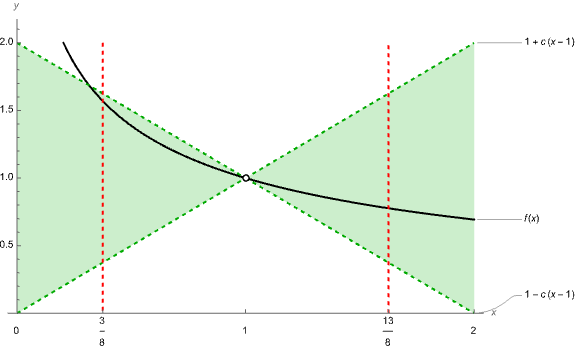
\includegraphics[width=6.5in]{img/power_series_and_limits1}
\caption{$f(x)=\DS\frac{\ln x}{x-1} = 1 + O(x-1)$ as $x\to 1$.}
\end{figure}

\newpage

\begin{example}
Use power series to evaluate the ``\textit{Mean Girls} limit"
$\DS\lim_{x\to 0}\frac{\ln(1-x)-\sin x}{1-\cos^2 x}$.
\end{example}
\ifdefined\SOLUTION
\SOLUTION{
Since the limit is indeterminate as $x\to 0$, we try expanding numerator and denominator as power series about $x=0$.
Recalling that
\begin{equation*}
\ln(1+x)=\sum_{k=1}^\infty(-1)^{k+1}\frac{x^k}{k}\quad (-1<x\le 1),
\end{equation*}
we deduce that
\begin{equation*}
\ln(1-x)=\sum_{k=1}^\infty(-1)^{k+1}\frac{(-x)^k}{k}
=-\sum_{k=1}^\infty\frac{x^k}{k}
\quad (-1\le x< 1).
\end{equation*}
Since 
\begin{equation*}
\sin x=\sum_{n=0}^\infty(-1)^n\frac{x^{2n+1}}{(2n+1)!}\quad (-\infty<x<\infty),
\end{equation*}
it follows that
\begin{equation*}
\ln(1-x)-\sin x=\left(-x-\frac{1}{2}x^2-\dots\right) - \left(x-\frac{1}{6}x^3+\dots\right)
=-2x+O(x^2)
\end{equation*}
as $x\to 0$.
Furthermore,
\begin{equation*}
\begin{split}
1-\cos^2(x)
=\sin^2(x)
&=\left(x-\frac{x^3}{6}+\dots\right)\left(x-\frac{x^3}{6}+\dots\right)\\
&=x^2 -\frac{1}{3}x^4+\dots\\
&=x^2+O(x^4)
\end{split}
\end{equation*}
as $x\to 0$.
Whence,
\begin{equation*}
\frac{\ln(1-x)-\sin x}{1-\cos^2 x}=\frac{-2x+O(x^2)}{x^2+O(x^4)}
=\frac{x}{x^2}\left(\frac{-2+O(x)}{1+O(x^2)}\right)
=\frac{1}{x}\left(\frac{-2+O(x)}{1+O(x^2)}\right)
\end{equation*}
as $x\to 0$, and therefore,
\begin{equation*}
\lim_{x\to 0}\frac{\ln(1-x)-\sin x}{1-\cos^2 x}
=\lim_{x\to 0}\frac{1}{x}\left(\frac{-2+O(x)}{1+O(x^2)}\right)\quad \text{DNE}.
\end{equation*}
}
\fi
\newpage

\begin{remark}\,
\begin{itemize}
\item The figure below illustrates a slightly stronger fact than what we proved in the previous exercise, namely,
\begin{equation*}
\frac{\ln(1-x)-\sin x}{1-\cos^2 x} = -\frac{2}{x} + O(1) \text{ as } x\to 0.
\end{equation*}
\item In particular, the plot suggests that if $0<|x|<3/4$, then
\begin{equation*}
\frac{\ln(1-x)-\sin x}{1-\cos^2 x} \approx -\frac{2}{x}
\end{equation*}
with an absolute error that is no worse than $2$.
\end{itemize}
\end{remark}

\begin{figure}[H]
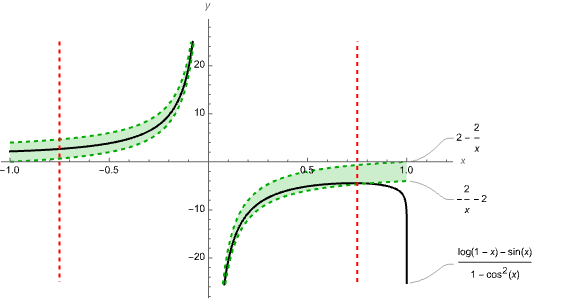
\includegraphics[width=6.5in]{img/power_series_and_limits2}
\caption{$f(x) =\DS\frac{\ln(1-x)-\sin x}{1-\cos^2 x} = -\frac{2}{x} + O(1)$ as $x\to 0$.}
\end{figure}

\newpage

\begin{remark}\,
\begin{itemize}
\item The classical (Newtonian) definition of the \textbf{kinetic energy} $K$ of an object with (a constant) mass $m$ moving with speed $v$ is
\begin{equation*}
K= \frac{1}{2}mv^2.
\end{equation*}
\item In the modern (Einsteinian) theory, the \textbf{rest energy} of an object with (rest) mass $m$ is defined by
\begin{equation*}
E_0 = mc^2
\end{equation*}
while the \textbf{total energy} of the object is defined by
\begin{equation*}
E = \gamma mc^2,
\end{equation*}
where
\begin{equation*}
\gamma = \frac{1}{\sqrt{1-(v/c)^2}}
\end{equation*}
is the \textbf{Lorentz factor}
and $c\approx 2.998\times 10^8$ \si{m/s} is the speed of light.
\item The \textbf{relativistic kinetic energy} of the object is then defined to be
\begin{equation*}
E_K = E-E_0.
\end{equation*}
\end{itemize}
\end{remark}

\begin{theorem}
As $v\to 0$,
\begin{equation*}
E_K = \frac{1}{2}mv^2 + O\big(v^4\big).
\end{equation*}
%i.e., there are constants $C,M>0$ so that 
%\begin{equation*}
%\left|E_K - \frac{1}{2}mv^2\right| < Cv^4
%\end{equation*}
%whenever $|v|<M$.
\end{theorem}
\begin{remark}
In other words, Newtonian kinetic energy is the ``first order approximation" to relativistic kinetic energy because it is the ``most significant term" in the Taylor series expansion for $E_K$ about $v=0$.
\end{remark}
\ifdefined\SOLUTION
\SOLUTION[Proof]{
The binomial theorem tell us that 
\begin{equation*}
\frac{1}{\sqrt{1+x}}=(1+x)^{-1/2}=\sum_{k=0}^\infty\binom{-1/2}{k}x^k = 1 - \frac{1}{2}x^2 + \frac{3}{8}x^4 + \dots \quad (-1 < x < 1).
\end{equation*}
Since the physicists tell us that $0< v < c$, we have that
\begin{equation*}
\gamma 
= \frac{1}{\sqrt{1-(v/c)^2}}
= 1 + \frac{1}{2}(v/c)^2 + O(v^4)
\end{equation*}
as $v\to 0$.
Whence,
\begin{equation*}
E_K = E - E_0 = (\gamma - 1)mc^2 = \frac{1}{2}mv^2 + O(v^4)
\end{equation*}
as $v\to 0$.
}
\else
\begin{proof}
\,
\vspace{3.1in}

\end{proof}
\fi

\newpage


\begin{definition}
If $z$ is complex number, we define
\begin{equation*}
\exp(z) = \sum_{n=0}^\infty \frac{z^n}{n!}.
\end{equation*}
\end{definition}

\begin{theorem}[Euler's identity]
For any real number $\theta$,
\begin{equation*}
\exp(\I\theta) = \cos\theta + \I\sin\theta,
\end{equation*}
where $\I$ is a square root of $-1$, i.e, $\I^2=-1$.
\end{theorem}
\ifdefined\SOLUTION
\SOLUTION[Proof]{
Note that $\I^2=-1, \I^3=-i, \I^4=1, \I^5=i, \I^6=-1,\dots$.
So we should separate odd and even powered terms.  
Therefore, if $\theta$ is real, then 
\begin{align*}
\E^{\I\theta}&=\sum_{n=0}^\infty \frac{(\I\theta)^n}{n!}\\
&=\sum_{n=0}^\infty\frac{\I^n\theta^n}{n!}\\
&=\sum_{m=0}^\infty\frac{\I^{2m}\theta^{2m}}{(2m)!}+\sum_{m=0}^\infty \frac{\I^{2m+1}\theta^{2m+1}}{(2m+1)!}\\
&=\sum_{m=0}^\infty\frac{(-1)^{m}\theta^{2m}}{(2m)!}+\sum_{m=0}^\infty \frac{\I(-1)^{m}\theta^{2m+1}}{(2m+1)!}\\
&=\cos\theta+\I\sin\theta.
\end{align*}
}
\else
\begin{proof}
\,
\vspace{4.5in}

\end{proof}
\fi
\newpage

\begin{example}
Express $\DS\int\sin x^2\dee x$ as a power series.
Then estimate $\DS\int_0^1\sin x^2\dee x$ to within $10^{-3}$.
\end{example}
\ifdefined\SOLUTION
\SOLUTION{
For all $x\in\mathbb{R}$, 
\begin{align*}
\int \sin(x^2)\dee x &= \int \sum_{n=0}^\infty\frac{(-1)^n(x^2)^{2n+1}}{(2n+1)!}\dee x
= \sum_{n=0}^\infty\frac{(-1)^n}{(2n+1)!} \int x^{4n+2}\dee x \\
&=  C + \sum_{n=0}^\infty\frac{(-1)^n}{(2n+1)!}\cdot\frac{x^{4n+3}}{4n+3}.
\end{align*}
So,
\begin{equation*}
\int_0^1 \sin(x^2)\dee x 
= \left.\sum_{n=0}^\infty\frac{(-1)^n}{(2n+1)!}\cdot\frac{x^{4n+3}}{4n+3}\right|_0^1
= \sum_{n=0}^\infty\frac{(-1)^n}{(2n+1)!(4n+3)}.
\end{equation*}
By ASET,
\begin{equation*}
|R_N|=\left|\sum_{n=N+1}^\infty\frac{(-1)^n}{(2n+1)!(4n+3)}\right|
<\left|\frac{(-1)^{N+1}}{(2N+3)!(4N+7)}\right|
=\frac{1}{(2N+3)!(4N+7)}.
\end{equation*}
Observe that $|R_1| < \frac{1}{5!\cdot 11}\approx 0.00076 < 10^{-3}$.
Therefore,
\begin{equation*}
\int_0^1 \sin{(x^2)}\dee x \approx S_1 
=\sum_{n=0}^1\frac{(-1)^n}{(2n+1)!(4n+3)}
=\frac{1}{3} - \frac{1}{3!\cdot 7} 
=\frac{1}{3} - \frac{1}{42} 
=\frac{13}{42}
\end{equation*}
is accurate to within $10^{-3}.$
}
\else
\fi

\setcounter{equation}{0}


%!TEX root =  main.tex
\setcounter{chapter}{11}
\setcounter{section}{1}
\setcounter{theorem}{0}
\setcounter{equation}{0}

\lectureheader{162}{Calculus II}{Parametric equations}{\textit{Thomas' Calculus}  \thesection}

\begin{definition}
Suppose that $x=f(t)$ and $y=g(t)$ are functions of some third variable $t$, called a \textbf{parameter}.
We say that $x$ and $y$ are given by \textbf{parametric equations}.
The set of points $(x,y)$ traced in the plane as $t$ varies is called a \textbf{parametric curve}.
\end{definition}

\begin{example}
Consider the curve given by the parametric equations
\begin{align*}
x&=t^2-2t,\\
y&=t+1
\end{align*}
for $t\in [0,\infty)$.
Plot the points on the curve corresponding to $t=0, 1, 2, 3$.
Then eliminate the parameter to and identify the curve and finish the sketch.
\end{example}

\ifdefined\SOLUTION
\SOLUTION{
We make a table of values:
\begin{center}
\begin{tabular}{c|c|c}
$t$ & $x$ & $y$\\
\hline
$0$ &  $0$ & $1$\\
$1$ & $-1$ & $2$\\
$2$ &  $0$ & $3$\\
$3$ &  $3$ & 4
\end{tabular}
\end{center}
Solving the equation $y=t+1$ for $t$ and substituting we have
\begin{equation*}
\begin{split}
x &= (y-1)^2 -2(y-1)\\
  &= y^2-4y+3.
\end{split}
\end{equation*}
Now as $t$ varies in the interval $[0,\infty)$, $y=t+1$ varies in the interval $[1,\infty)$.
Therefore, the parametric equations trace out 
\begin{equation*}
x = y^2-4y+3\quad (1\le y<\infty).
\end{equation*}
This is part of a parabola that opens toward the right.
However, the parametrization also imposes an orientation: 
the parabola is traversed from the point $(x,y)=(0,1)$ upwards.
}
\fi

\newpage

\begin{example}
Consider the curve given by the parametric equations
\begin{align*}
x &= t + \frac{1}{t},\\
y &= t - \frac{1}{t} \quad (t>0).
\end{align*}
Eliminate the parameter to identify the curve.
\end{example}

\ifdefined\SOLUTION
\SOLUTION{
Adding the equations, we find that
\begin{equation*}
x+y = 2t,
\end{equation*}
and subtracting the equation, we have
\begin{equation*}
x-y = \frac{2}{t}.
\end{equation*}
Multiplying these two new equations, we find that
\begin{equation*}
x^2-y^2 = (x+y)(x-y) = 2t\frac{2}{t} = 4.
\end{equation*}
As $t$ varies in the interval $(0,\infty)$, 
we see that $x=t + 1/t$ also varies in the interval $(0,\infty)$ and $y=t-1/t$ varies in the interval $(-\infty,\infty)$.
Therefore, the parametric equations trace out the right half of the hyperbola
\begin{equation*}
x^2-y^2 = 4 \quad (x>0)
\end{equation*}
but it does so from bottom to top.
}
\fi

\newpage

\begin{remark}\,
\begin{enumerate}
\item One advantage of parametric equations is their ``explicit" (as opposed to ``implicit") nature.
\begin{enumerate}
\item To find a point on the curve given by 
\begin{equation*}
\frac{x^2}{16}+\frac{y^2}{9}=1,
\end{equation*}
we have to pick a value for one of the variables and then \underline{try} to solve for the other.
\item To find a point on the curve given by
\begin{align*}
x &=  4\cos t,\\
y &=  3\sin t\quad (0\le t\le 2\pi)
\end{align*}
we simply choose any $t\in [0,2\pi]$, and we immediately get a point on the curve every time.
\end{enumerate}
\item Another advantage of parametrization is that it imposes ``orientation" on a curve (direction of traverse) which some applications require.
For example, we may want to model the``position" of some object that depends on some non-spatial parameter (e.g., time).
\item A third advantage of parametrization is that each coordinate is given as a function of the parameter $t$, and it is far easier to apply the tools of calculus to functions.
\end{enumerate}
\end{remark}

\newpage

\begin{example}
Two particles start at the same instant in time.
The first travels along the path 
\begin{equation*}
C_1: x = \frac{16}{3}-\frac{8}{3}t,\quad y = 4t-5 \quad (t\ge 0)
\end{equation*}
while the second travels along the path 
\begin{equation*}
C_2: x = 2\sin\left(\frac{\pi}{2}t\right),\quad y = -3\cos\left(\frac{\pi}{2}t\right) \quad (t\ge 0).
\end{equation*}
At what points, if any, do the paths intersect?  At what points, if any, do the particles collide?
\end{example}

\ifdefined\SOLUTION
\SOLUTION{
The equations for $C_1$ may be rewritten as
\begin{align*}
3x &= 16 - 8t,\\
2y &= 8t - 10.
\end{align*}
Adding these equations, we find that
\begin{equation*}
3x+2y = 6\quad (y\ge -5),
\end{equation*}
which is a ``half-line."
The equations for $C_2$ may be rewritten as $C_2$ as
\begin{align*}
\frac{x}{2} &= \sin\left(\frac{\pi}{2}t\right),\\
\frac{y}{-3}&= \cos\left(\frac{\pi}{2}t\right).
\end{align*}
Whence, squaring and adding, the usual Pythagorean identity gives
\begin{equation*}
\frac{x^2}{4} + \frac{y^2}{9} = 1,
\end{equation*}
which is an ellipse that is traversed counterclockwise infinitely many times starting at the point $(x,y) = (0,-3)$.
To determine if the curves intersect, we simultaneously solve the cartesian equations.
We rewrite the cartesian equation for $C_1$ as $3x = 6-2y$ 
and the cartesian equation for $C_2$ as $(3x)^2 + 4y^2 = 36$.
Substituting the first into the later, we have
\begin{equation*}
(6-2y)^2 +4y^2 = 36.
\end{equation*}
Expanding, we have 
\begin{equation*}
36 - 24y + 8y^2 = 36.
\end{equation*}
Whence,
\begin{equation*}
8y(y-3) = 0,
\end{equation*}
and so $y=0$ or $y=3$.
Substituting these values back into the equation for $C_1$, we find that $x=2$ in the first case and $x=0$ in the latter.
Therefore, the curves intersect at $(x,y)=(2,0)$ and $(x,y)=(0,3)$.
The particle on $C_1$ is at $(x,y)=(2,0)$ if and only if $t=5/4$, and it is at $(x,y)=(0,3)$ if and only if $t=2$.
When $t=5/4$, the particle on $C_2$ is at $(x,y) = \Big(2\sin(5\pi/8), -3\cos(5\pi/8)\Big)\ne (2,0)$.
So the particles do not collide at $(2,0)$.
However, when $t=2$, the particle on $C_2$ is at $(x,y) = (0,3)$, and so the particles do collide at this point.
}
\fi

\newpage

\begin{remark}
The following ``bread and butter" parametrizations are important to know.
\begin{itemize}
\item
Given distinct points $(a,b), (c,d)\in\R^2$, the unique line passing through $(a,b)$ and $(c,d)$ may be parametrized by the equations
\begin{align*}
x & = a(1-t) + ct,\\
y &=  b(1-t) + dt
\end{align*}
for $t\in (-\infty, \infty)$.
%\begin{remark}
%The line segment \underline{from} $(a,b)$ \underline{to} $(c,d)$ is traversed as $t$ varies in $[0,1]$.
%\end{remark}
\item
Given $a, b\in \R$, the ellipse
\begin{equation*}
\frac{x^2}{a^2}+\frac{y^2}{b^2}=1
\end{equation*}
is parametrized with counterclockwise orientation by the equations
\begin{align*}
x & = a\cos t,\\
y &= b\sin t
\end{align*}
for $t\in [0,2\pi]$.
\item
Given $a, b\in \R$, the hyperbola
\begin{equation*}
\frac{x^2}{a^2}-\frac{y^2}{b^2}=1
\end{equation*}
is parametrized by the equations
\begin{align*}
x & = a\sec t,\\
y &= b\tan t
\end{align*}
for $t\in [0,2\pi]$.
\item
Given $a, b\in \R$, the right branch of the hyperbola
\begin{equation*}
\frac{x^2}{a^2}-\frac{y^2}{b^2}=1
\end{equation*}
is parametrized by the equations
\begin{align*}
x & = a\cosh t,\\
y &= b\sinh t
\end{align*}
for $t\in (-\infty,\infty)$.
\item If $y=f(x)$ is a function of $x$, then the curve
\begin{equation*}
y=f(x)\quad (a\le x\le b)
\end{equation*}
is parametrized by the equations
\begin{align*}
x &= t,\\
y &=f(t)
\end{align*}
for $t\in [a,b]$.
\end{itemize}
\end{remark}


\setcounter{equation}{0}

%!TEX root =  main.tex

\lectureheader{162}{Calculus II}{Calculus on parametric equations}{\textit{Thomas' Calculus} \textsection 11.2}

\begin{theorem}
If $x$ and $y$ are given as functions of the parameter $t$, then
\begin{equation*}
\frac{\dee y}{\dee x} = \frac{\frac{\dee y}{\dee t}}{\frac{\dee x}{\dee t}}
\end{equation*}
whenever $\frac{\dee x}{\dee t}\ne 0$.
\end{theorem}

\begin{example}
Find the tangent line to the curve
\begin{align*}
x &= \sec t,\\
y &= \tan t
\end{align*}
at the point $(\sqrt 2, 1)$, i.e., when $t=\pi/4$.
\end{example}

\newpage

\begin{example}
Compute $\frac{\dee^2 y}{\dee x^2}$ as a function of $t$ is
\begin{align*}
x & = t-t^2,\\
y &= t-t^3.
\end{align*}
\end{example}

\newpage

\begin{remark}\,
\begin{itemize}
\item The substitution rule (i.e., chain rule in reverse) can help us compute areas in parametric form as well.
\item If $y$ is a function of $x$ and $x$ is a function of $t$, then
\begin{equation*}
\int_{x(a)}^{x(b)}y\dee x = \int_a^b y(t)\frac{\dee x}{\dee t}\dee t.
\end{equation*}
\end{itemize}
\end{remark}

\begin{example}
Find the area enclosed by the astroid
\begin{align*}
x &= \cos^3 t,\\
y &= \sin^3 t\quad (0\le t\le 2\pi).
\end{align*}
\begin{flushright}
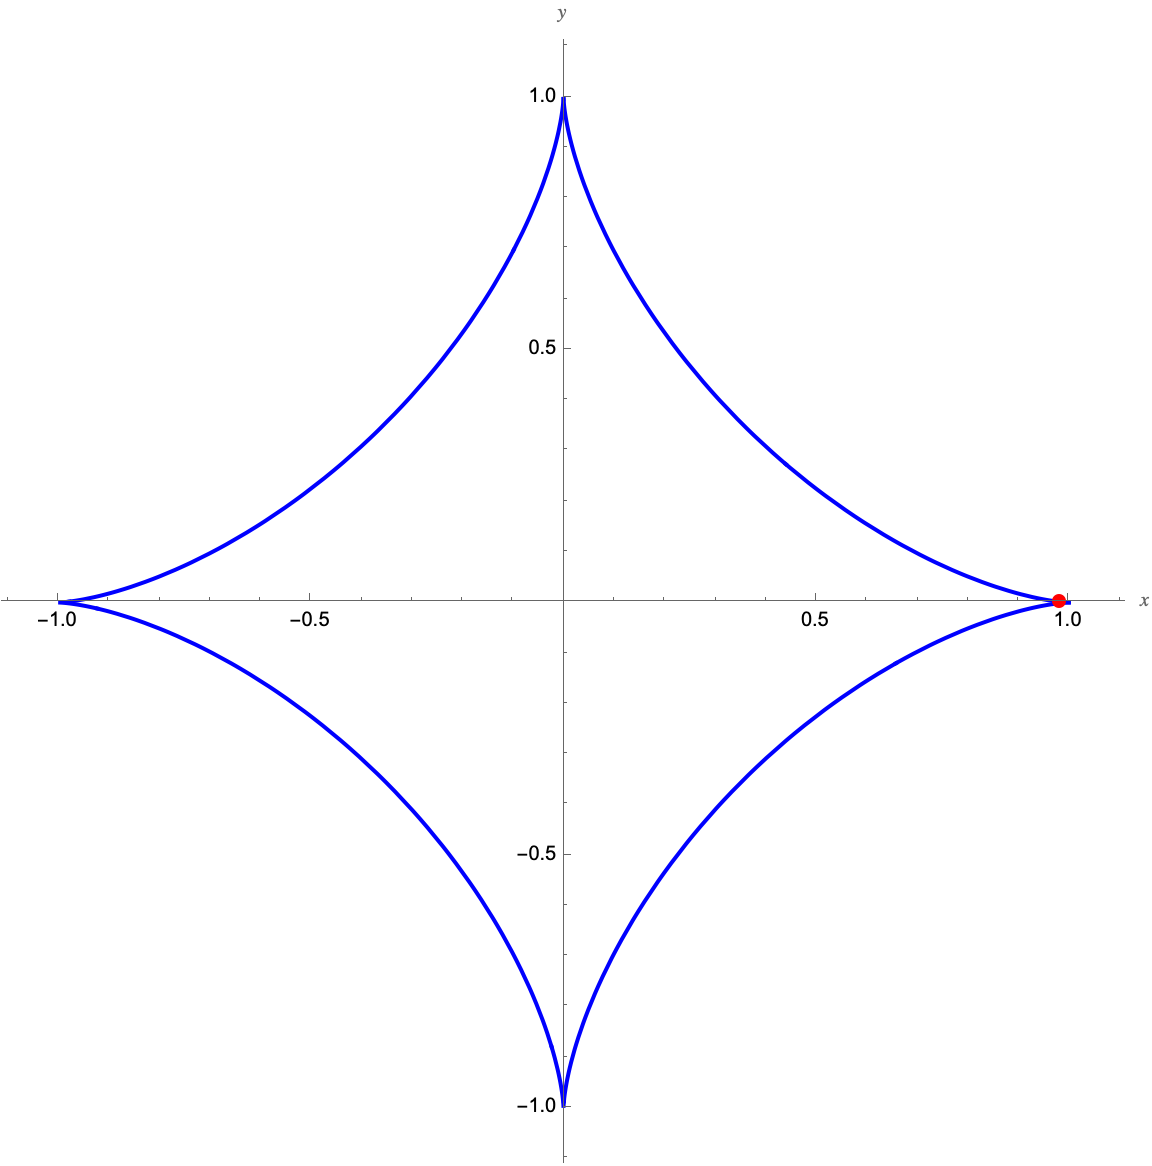
\includegraphics[width=2.5in]{img/astroid}
\end{flushright}
\end{example}

\newpage

\begin{definition}
Given a parametric curve $C$ that is traversed exactly once as $t$ varies from $\alpha$ to $\beta$, we define the \textbf{arc length differential} by
\begin{equation*}
\dee s = \sqrt{\dee x^2 + \dee y^2},
\end{equation*}
and we define the \textbf{arc length} of $C$ by
\begin{equation*}
s = \int_C\dee s = \int_\alpha^\beta\sqrt{\left(\frac{\dee x}{\dee t}\right)^2 + \left(\frac{\dee y}{\dee t}\right)^2}\dee t
\end{equation*}
provided that the integral exists.
\end{definition}

\begin{remark}\,
\begin{itemize}
\item It is tradition to denote arc length by $s$ for the Latin \textit{spatium}.
\item The definition of $\dee s$ is based on the distance formula and is meant to signify an ``infinitesimal" distance traveled \textit{along} the curve $C$.  
\item In particular, if $C$ passes through the points $(x_{i-1}, y_{i-1})$ and $(x_i, y_i)$, then then distance $\Delta s_i$ traveled \textit{along} $C$ between these two points may be approximated by the straight line distance between the two points, i.e.,
\begin{equation*}
\Delta s_i \approx \sqrt{\Delta x_i^2 + \Delta y_i^2},
\end{equation*}
where $\Delta x_i = x_i-x_{i-1}$ and $\Delta y_i = y_i - y_{i-1}$.
\item Observe that $\dee s$ has the correct units of length attached to it.
\end{itemize}
\end{remark}

\newpage

\begin{example}
Compute the length of the astroid
\begin{align*}
x &= \cos^3 t,\\
y &= \sin^3 t\quad (0\le t\le 2\pi).
\end{align*}
\end{example}

\newpage



\begin{definition}
Suppose that the parametric curve $C$ is traversed exactly once as $t$ varies from $\alpha$ to $\beta$.
If $C$ is rotated about the $x$-axis to generate a surface of revolution $S$, we define the \textbf{(surface) area} $A$ of the resulting \textit{surface of revolution} by
\begin{equation*}
A = \int_C 2\pi y\dee s =2\pi \int_\alpha^\beta y(t)\sqrt{\left(\frac{\dee x}{\dee t}\right)^2 + \left(\frac{\dee y}{\dee t}\right)^2}\dee t
\end{equation*}
provided that the integral exists.
\end{definition}

\begin{remark}\,
\begin{itemize}
\item If $C$ is rotated about the $y$-axis, then 
\begin{equation*}
A = \int_C 2\pi x\dee s =2\pi \int_\alpha^\beta x(t)\sqrt{\left(\frac{\dee x}{\dee t}\right)^2 + \left(\frac{\dee y}{\dee t}\right)^2}\dee t.
\end{equation*}
\item The definition is based off the area of the \textit{frustum} of a cone.
\item Observe that, in either case, $A$ has the correct dimensionality.
\end{itemize}
\end{remark}

\newpage

\begin{example}
Calculate the area of the surface that is generated by rotating the curve $y=\sqrt{4-x^2}$ for $-1\le x\le 1$ about the $x$-axis.
\end{example}

\newpage

\begin{example}
Show that Gabriel's horn has infinite surface area despite having finite volume.
\end{example}


\setcounter{equation}{0}


\end{document}
